%!TEX root = ../dissertation.tex
\begin{savequote}[75mm]
Even in the darkest night. Stars and angels still shine bright.   
\qauthor{Bear}
\end{savequote}


\chapter{Background Estimation}

\section{Overview}
\paragraph{}
The invariant mass of the two-Higgs-boson-candidate system, \mtwoJ, is used as the final discriminant between Higgs boson pair production and the SM backgrounds.
Multi-jet (QCD) is the dominant background.
About $40\%$ the QCD events are $gg \to b\bar{b}b\bar{b}$, and $60\%$ $gg \to c\bar{c}c\bar{c}$ or $gg \to q\bar{q}q\bar{q}$ fakes multiple $b$s.
There is no accurate nor high-statistics MC with three or four $b$-jets collected into two high-\pt~ large-\R jets.
Therefore, a data-driven method is used for estimating both the yield and kinematic distribution of the QCD events.
For \ttbar~ background, reasonably sized MC samples are available. 
They provide \ttbar~ kinematic distributions.
The \ttbar~ yield is also estimated using a data-driven method to avoid mis-modeling in the MC.
The $Z$+jets background is small, and it estimated by the $Z$+heavy flavor jets MC.
The SM $ZZ\to b\bar{b}b\bar{b}$ has been estimated to be completely negligible using a particle-level analysis.
For the three signal regions in number of $b$-tags, the fraction of expected backgrounds are:
\begin{itemize}
	\item $4b$: QCD $\sim 95\%$, $t\bar{t}$ $\sim 5\%$, $Z$+jets$< 1\%$. 
	\item $3b$: QCD $\sim 90\%$, $t\bar{t}$ $\sim 10\%$, $Z$+jets $< 1\%$.  
	\item $2bs$: QCD $\sim 80\%$, $t\bar{t}$ $\sim 20\%$, $Z$+jets $< 1\%$.
\end{itemize}

\paragraph{}
The shapes of the QCD background is estimated from signal depleted data regions. 
These regions are selected with the signal region selection, except they must have lower number of $b$-tagged track jets.
The differences in kinematic distributions between the lower-tagged and $n$-tag regions are corrected by reweighting the lower-tagged sample.

\paragraph{}
The less $b$-tagged regions only estimate the shapes of the expected background, but not the total yield.
The \textit{sideband region} (SB), with the same number of $b$-tags as the signal regions but a cut on \mleadJ-\msublJ different from the $X_{hh}$ cut, is used to estimate the yield.
A third region, called the \textit{control region} (CR), is used to validate the background estimations.
The sideband and control regions are optimized to accurately estimate the rate of QCD and \ttbar~ background. 

\paragraph{}
The definition of SB and CR is introduced in section~\ref{sec:boosted-SBCR}.
The QCD and \ttbar~ background shape templates are introduced in section~\ref{sec:boosted-qcd} and section~\ref{sec:boosted-ttbar}.
The normalization estimation for QCD and \ttbar~ is introduced in section~\ref{sec:ttbarnorm}.
The reweighting procedure is explained in section~\ref{sec:boosted-reweight}.
The SR prediction is further rescaled and smoothed, discussed in section~\ref{sec:boosted-SR-smoothing}.
The SB and CR distributions are shown in section~\ref{sec:boosted-sb}, section~\ref{sec:boosted-cr}. 
The yields are listed section~\ref{sec:yields}.

%%%%%%%%%%%%%%%%%%%%%%%%%%%%%%%%%%%%%%%%%%%%%%%%%%%%%%%%%%%%%%%%%%%%%%%
%%%%%%%%%%%%%%%%%%%%%%%%%%%%%%%%%%%%%%%%%%%%%%%%%%%%%%%%%%%%%%%%%%%%%%%
%%%  SB. CR
%%%%%%%%%%%%%%%%%%%%%%%%%%%%%%%%%%%%%%%%%%%%%%%%%%%%%%%%%%%%%%%%%%%%%%%
%%%%%%%%%%%%%%%%%%%%%%%%%%%%%%%%%%%%%%%%%%%%%%%%%%%%%%%%%%%%%%%%%%%%%%%

\section{Definition of the sideband and control regions}
\label{sec:boosted-SBCR}

\paragraph{}
A circular variable $R_{hh}$ is defined in the 2D \mleadJ-\msublJ mass plane. 
It has the same central values as $X_{hh}$, but without resolution terms in the denominators:
\begin{equation}
\label{eq:boosted_RhhDef}
R_{hh} = \sqrt{\left(m^{\rm lead}_{\rm J} - \text{124 GeV}\right)^2 + \left(m^{\rm subl}_{\rm J} - \text{115 GeV}\right)^2}
\end{equation}

\paragraph{}
Similarly, $R_{hh}^{\text{high}}$, the circular region with the previous central values shifted up by $10$ \GeV, is defined as:
\begin{equation}
\label{eq:boosted_RhhhighDef}
R_{hh}^{\text{high}} = \sqrt{\left(m^{\rm lead}_{\rm J} - \text{134 GeV}\right)^2 + \left(m^{\rm subl}_{\rm J} - \text{125 GeV}\right)^2}
\end{equation}

\paragraph{}
The definitions of the SB, CR, and SR in the 2D \mleadJ-\msublJ plane are listed in Table~\ref{tab:boosted-sbcr-constraints}.
These regions are shown in Figure~\ref{fig:boosted-region-def}.
This Figure also shows the QCD background rate is decreasing from the low \mleadJ-\msublJ mass region to high \mleadJ-\msublJ mass region on the 2D plane.
The \ttbar~ background is also distinguishable as the vertical cyan band where \mleadJ $\sim 173$ \GeV.

\begin{table}[htbp!]
\begin{center}
\caption{Definitions of the signal region, the control region and the sideband region.}
\begin{tabular}{c|c}
\hline
  Region                                      & Definition \\
  \hline
  Signal region (SR) & $X_{hh}$ < 1.6\\
  control region (CR) & $R_{hh}$ < 33~\GeV\ and $X_{hh}$ > 1.6 \\
  sideband region (SB) & 33~\GeV < $R_{hh}$ and $R_{hh}^{\text{high}}$ < 58~\GeV
  \end{tabular}
\label{tab:boosted-sbcr-constraints}
\end{center}
\end{table}


\paragraph{}
The CR is as close to the signal region as possible.
The ring shape around the SR allows a good test for the background predictions with all \mleadJ-\msublJ combinations, and avoids too few or too many \ttbar~ events.
The current CR gives $N_{CR} \sim 2 N_{SR}$, which contains good statistics, and not affecting the SB design.

\paragraph{}
The SB must be a reasonable approximation for the QCD events contained in the CR and SR.
It is therefore chosen as the ring outside the CR regions.
The shift upwards in $R_{hh}^{\text{high}}$ center helps to contain enough \ttbar~ events in the normalization estimates.
%Different Large-\R jet mass reflects very different underlying kinematics.
A larger SB will potentially increase the kinematic differences between different QCD processes in CR/SR and SB.
Intrinsically, different \mleadJ-\msublJ reflects of different portion of $g \to b\bar{b}$ and $g \to c\bar{c}/q\bar{q}$ events.
This kinematic bias should be reduced as much as possible.
A smaller SB will introduce larger statistical uncertainties in the normalization estimation.
This is a bias variance trade off.
The current design gives roughly $N_{SB} \sim 4 N_{SR}$ and $N_{SB} \sim 2 N_{CR}$, which provides a good balance of the bias and variance in the background estimation.

\begin{figure*}[htbp!]
\begin{center}
  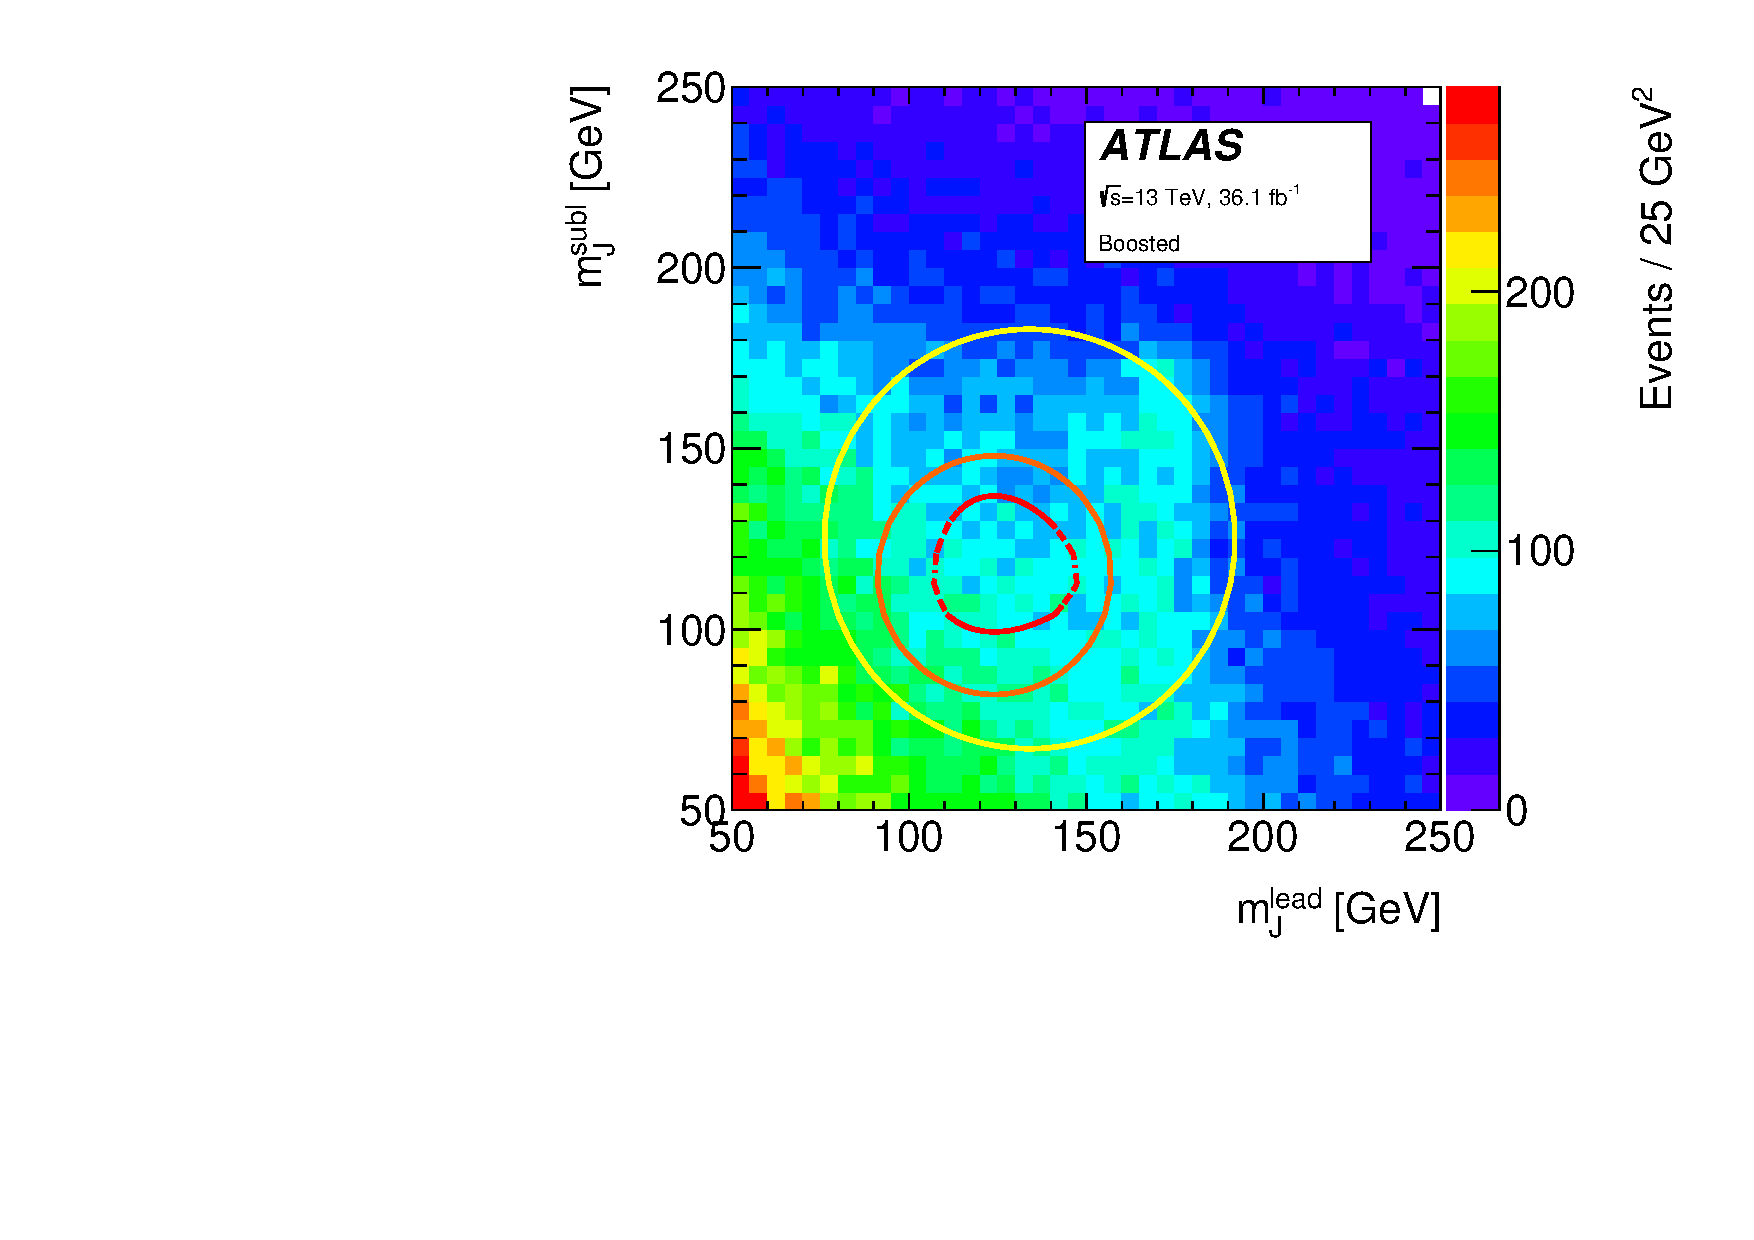
\includegraphics[width=0.6\textwidth,angle=-90]{figures/boosted/Other/TwoTag_split_Incl_data_mH0H1.pdf}
  \caption{The \mleadJ vs \msublJ distribution of the $2bs$ data. The signal region is the area surrounded by the inner (red) dashed contour line, centered on (\mleadJ=124~\GeV, \msublJ=115~\GeV). The control region is the area between the signal region and the intermediate (orange) contour line. The sideband region is the area between the control region and the outer (yellow) contour line.}
  \label{fig:boosted-region-def}
\end{center}
\end{figure*}

\paragraph{}
The fraction of expected events in the control region and sideband region as a function of \Grav~ Resonance mass is shown in Figure~\ref{fig:boosted-selection-region-efficiency}. 
For $4b$, $3b$, and $2bs$, there is no significant signal contamination in the control and sideband regions.


\begin{figure}[htbp!]
  \centering
  \captionsetup{justification=centering}
    \begin{subfigure}[b]{0.4\textwidth}
        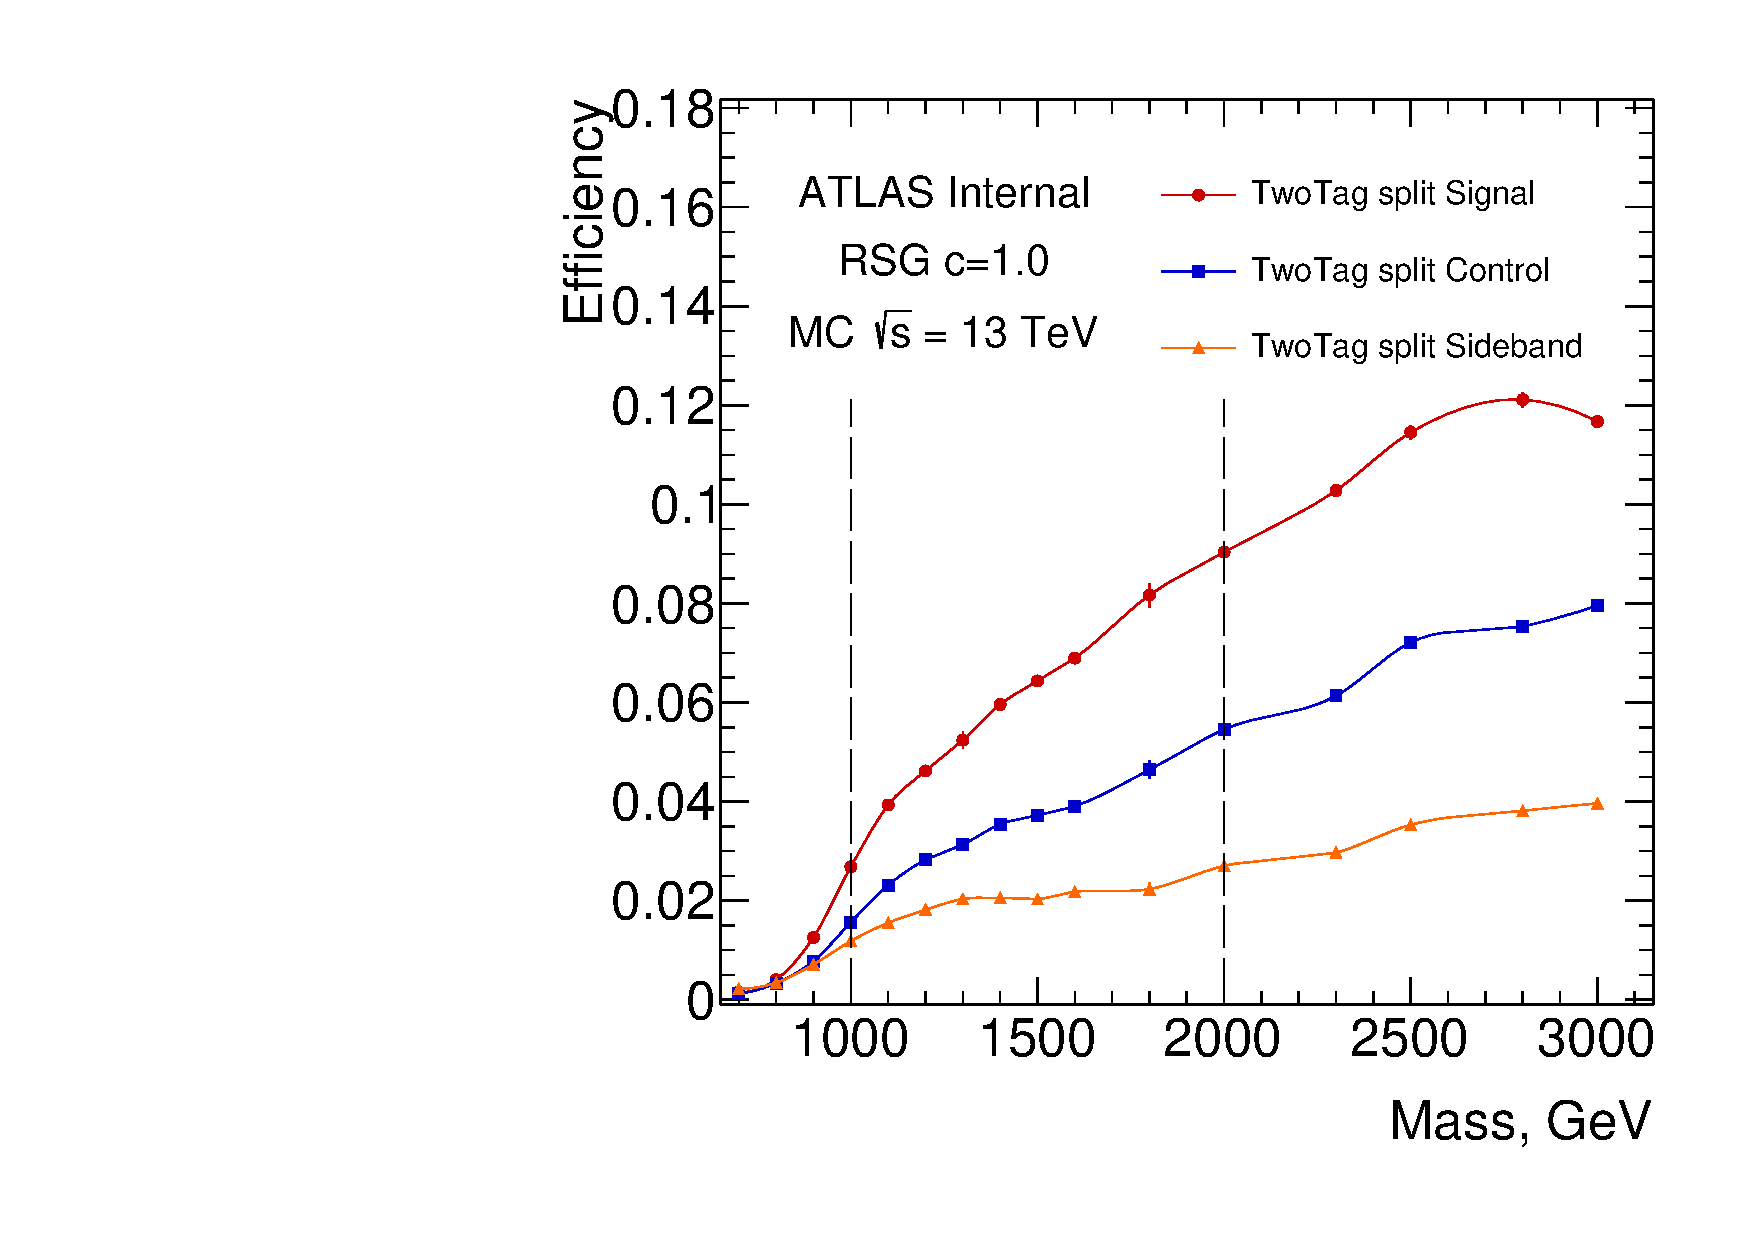
\includegraphics[width=\textwidth,angle=-90]{figures/boosted/SigEff/region_2b_lst_Moriond_Efficiency_PreSel.pdf}
        \caption{$2bs$ regions}
        \label{fig:2bs-selection-region-efficiency}
    \end{subfigure}
    \quad \quad 
    \begin{subfigure}[b]{0.4\textwidth}
        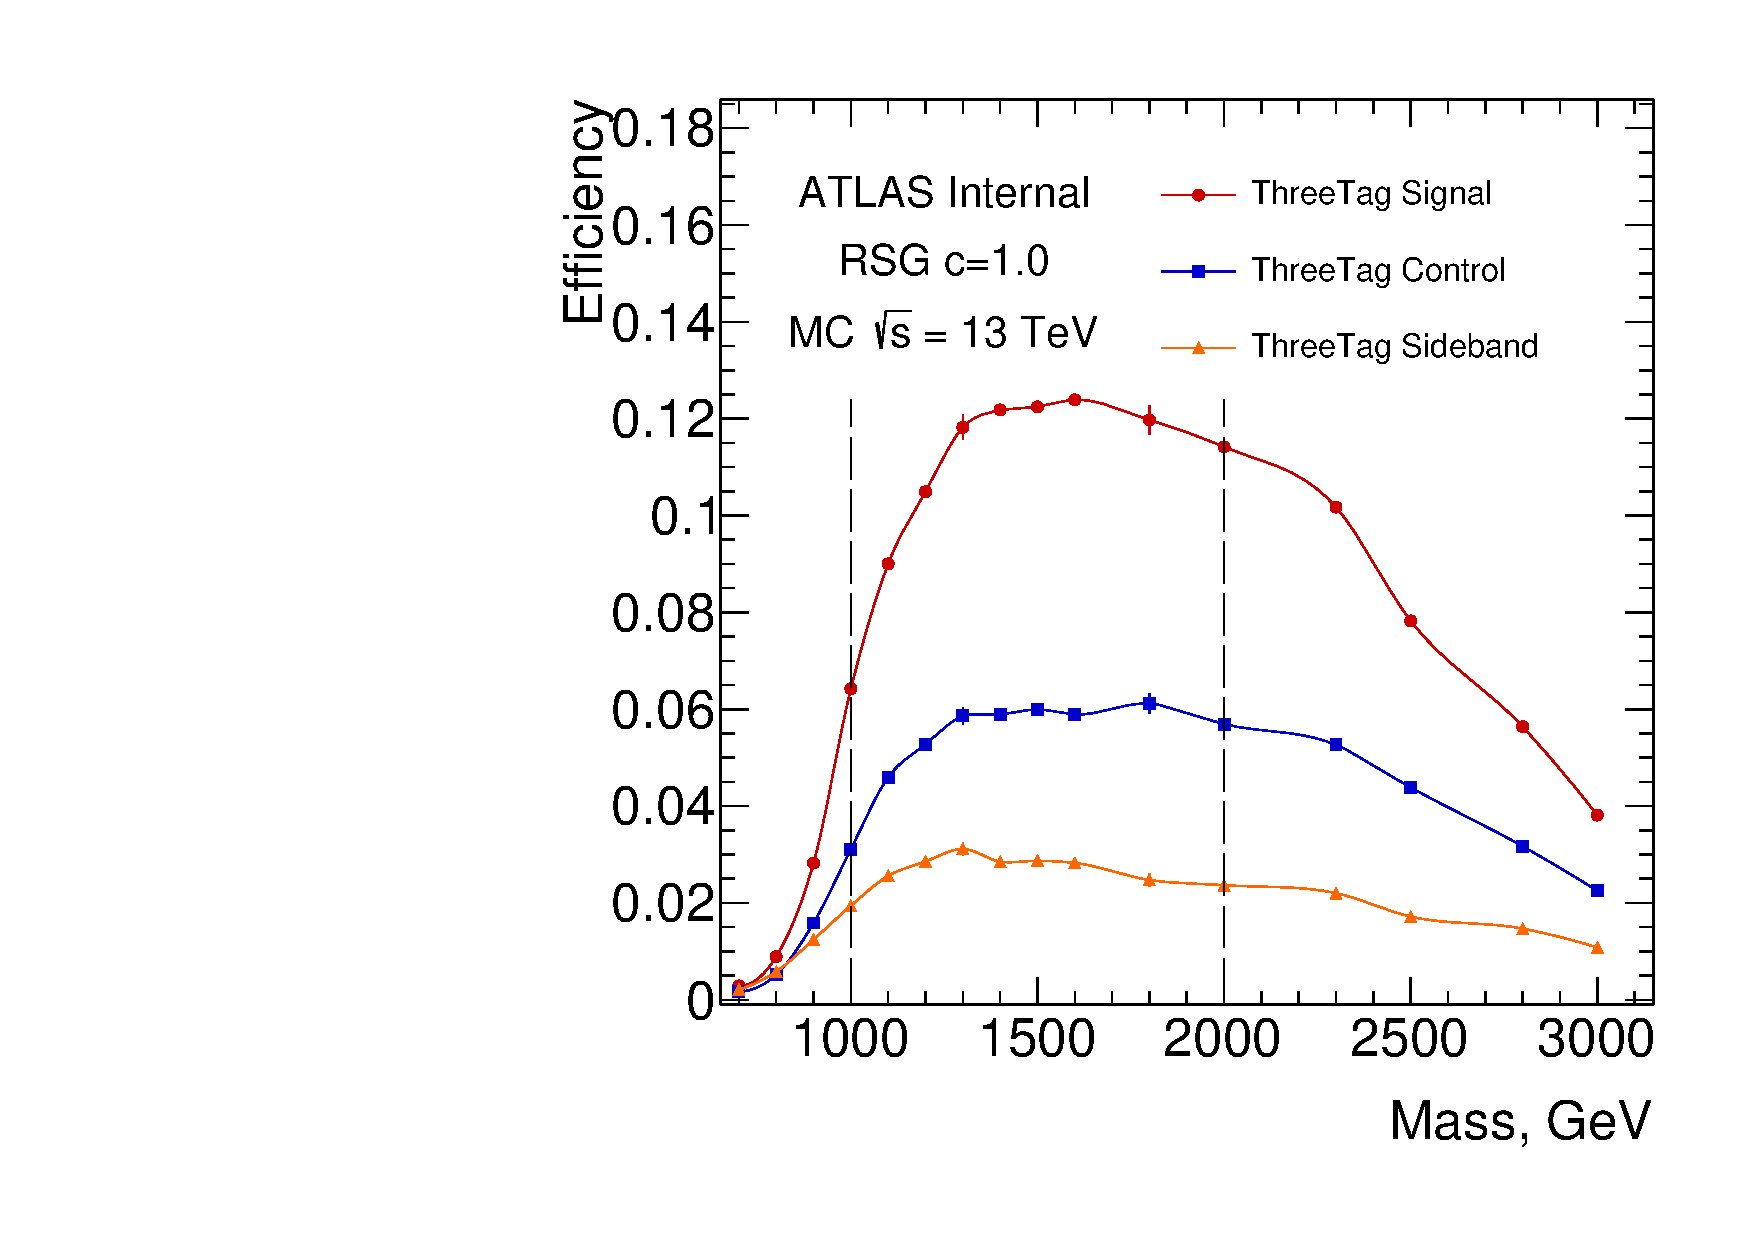
\includegraphics[width=\textwidth,angle=-90]{figures/boosted/SigEff/region_3b_lst_Moriond_Efficiency_PreSel.pdf}
        \caption{$3b$ regions}
        \label{fig:3b-selection-region-efficiency}
    \end{subfigure} \\ 
    \begin{subfigure}[b]{0.4\textwidth}
        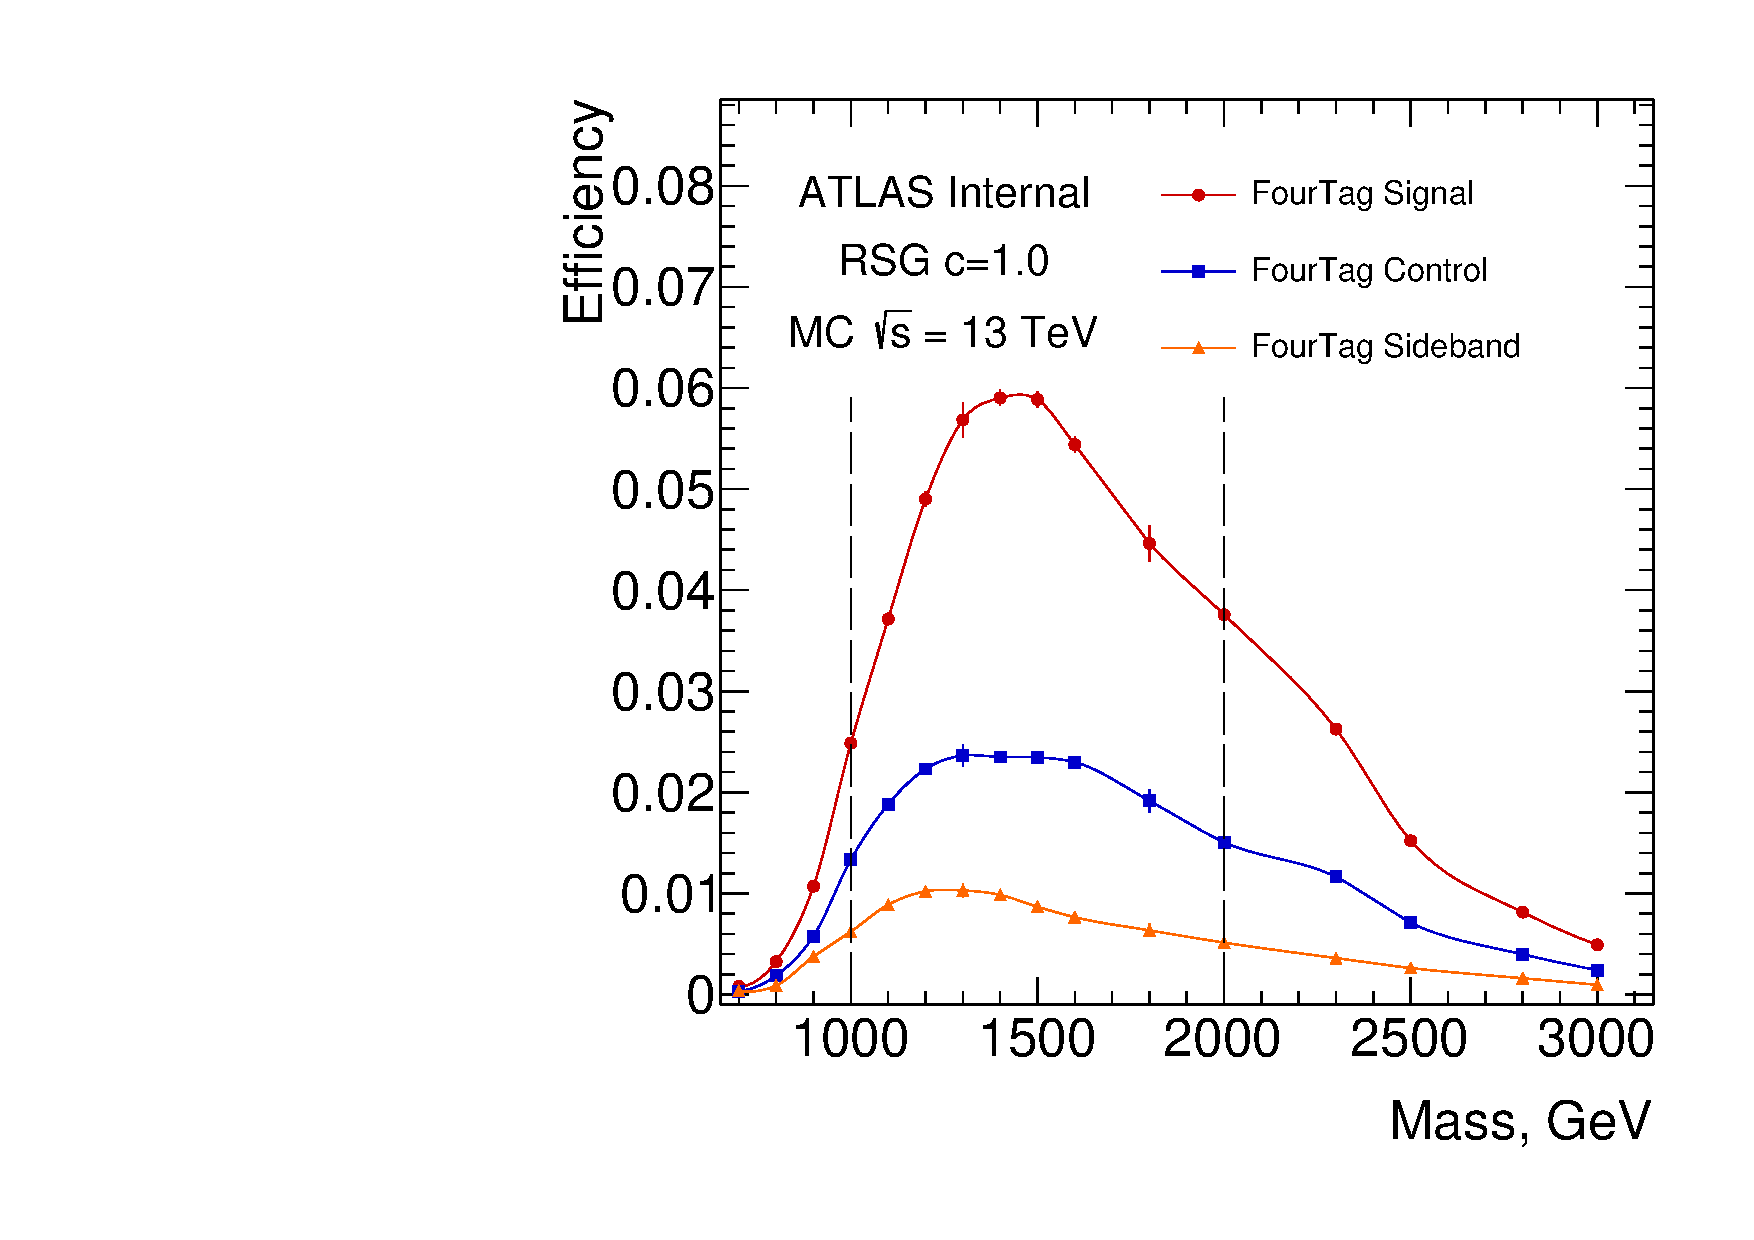
\includegraphics[width=\textwidth,angle=-90]{figures/boosted/SigEff/region_4b_lst_Moriond_Efficiency_PreSel.pdf}
        \caption{$4b$ regions}
        \label{fig:4b-selection-region-efficiency}
    \end{subfigure}
    \quad \quad 
    \begin{subfigure}[b]{0.4\textwidth}
        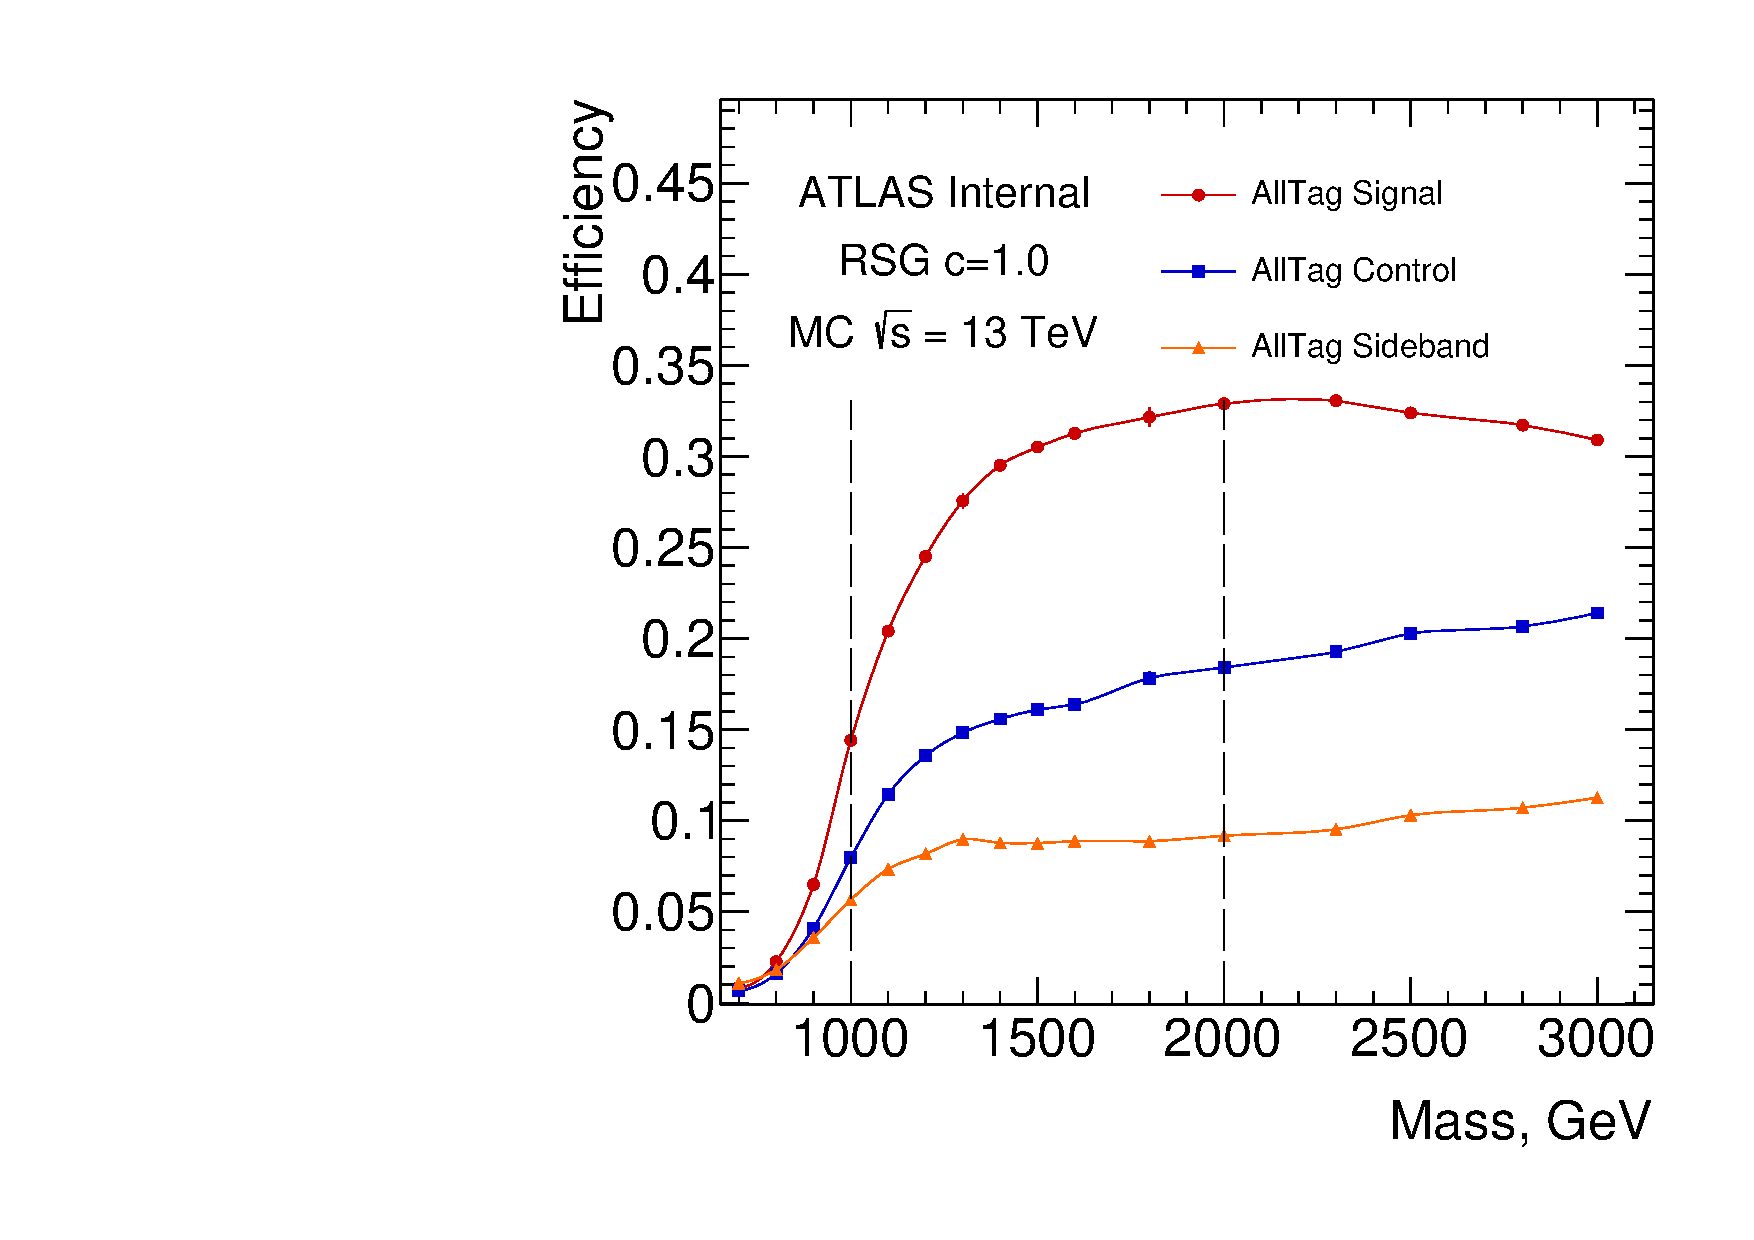
\includegraphics[width=\textwidth,angle=-90]{figures/boosted/SigEff/region_alltag_lst_Moriond_Efficiency_PreSel.pdf}
        \caption{Inclusive regions}
        \label{fig:alltag-selection-region-efficiency}
    \end{subfigure} \\ 
   \caption{
   Detailed signal efficiency in different signal/control/sideband regions as in $n$-tag regions and inclusive b-tagged regions, which include $2b$, $1b$ and 0$b$ as well, (bottom right) as a function of \Grav~ resonance mass for selection cuts. The efficiencies are relative to the total number of events in the preselection.}
  \label{fig:boosted-selection-region-efficiency}
\end{figure}


%%%%%%%%%%%%%%%%%%%%%%%%%%%%%%%%%%%%%%%%%%%%%%%%%%%%%%%%%%%%%%%%%%%%%%%
%%%%%%%%%%%%%%%%%%%%%%%%%%%%%%%%%%%%%%%%%%%%%%%%%%%%%%%%%%%%%%%%%%%%%%%
\section{QCD multi-jets}
\label{sec:boosted-qcd}

\paragraph{}
The QCD multi-jets prediction relies on finding regions that are similar in signal region event properties.
These regions are defined to be identical to the signal regions except requiring fewer number of $b$-tagged track jets associated with the large-\R jets.
They are orthogonal to the $n$-tag regions with no overlapping events:
\begin{itemize}
\item For the $2bs$ category, $1b$ data events, where one large-\R jet has one and only one $b$-tagged track jets, and the other large-\R jet has no $b$-tagged track jet, is used for modeling.
\item For the $3b$ and $4b$ categories, $2b$ data events, where one large-\R jet has two $b$-tagged track jets, and the other large-\R jet has no $b$-tagged track jet, is used for modeling. The $2b$ sample is further split into $80\%-20\%$ parts, where each is used separately for $3b$ and $4b$ background estimations. This ensures the shape estimations of $3b$ and $4b$ QCD estimates are uncorrelated. 
\end{itemize}
The $1b/2b$ MC predicted $t\bar{t}$ and $Z$+jets events in the $1b/2b$ regions are subtracted from the data distributions to produce the QCD estimation. 
Therefore, the number of QCD events, $N_{\text{qcd}}$, is estimated in Equation~\ref{eq:nqcd}.
\begin{eqnarray}
\label{eq:nqcd}
N_{\text{qcd}} = N_{\text{data}} - N_{t\bar{t}} - N_{Z+jets} 
\end{eqnarray}

\paragraph{}
The $1b$-tagged region also requires that each large-\R jet has at least one track jet (to model $2bs$).
Similarly, to model $3b$, the $2b$-tagged region requires that one large-\R jet has at least one track jet and the other one has at least two track jets. 
To model $4b$, each large-\R jet must have at least two track jets (to model $4b$).
This prevents biases in \mtwoJ~ distribution from the number of associated track jets.

\paragraph{} 
The resolved signal region events veto impacts the $4b$ background estimation. 
To account for this effect, a part of $2b$ data events used for $4b$ background estimation are excluded.
The vetoed events must have at least two small-\R jets that are $b$-tagged (passing the resolved $70\%$ $b$-tagging working point), and in case where the two other non $b$-tagged resolved jets can make a Higgs candidate, must pass the $X_{hh-resolved} < 1.6$ cut.
This ensures that a similar sculpting effect from the resolved veto is reflected in the background estimation in $4b$ signal region.
This reduces the estimated number of events in the signal region by $10\$$.

\paragraph{}
Given the $1b/2b$ QCD background shape predictions, the normalization of the QCD background is determined in the sideband by fitting the \mleadJ distribution simultaneously with QCD and \ttbar~ background templates, as described in section~\ref{sec:ttbarnorm}.
There are kinematic differences between the $1b/2b$ samples and the $4b/3b/2bs$ regions.  
A kinematic reweighting is applied to correct for such differences, as described in Section~\ref{sec:boosted-reweight}.


%%%%%%%%%%%%%%%%%%%%%%%%%%%%%%%%%%%%%%%%%%%%%%%%%%%%%%%%%%%%%%%%%%%%%%%
%%%%%%%%%%%%%%%%%%%%%%%%%%%%%%%%%%%%%%%%%%%%%%%%%%%%%%%%%%%%%%%%%%%%%%%
\section{\ttbar~}
\label{sec:boosted-ttbar}

\paragraph{}
The \ttbar~ events in the signal region mainly decay to $W^{\pm}$s that further decay hadroniclly.
The \ttbar~ MC is scaled by the luminosity in the data.
The boosted event selection on is applied on the \ttbar~ MC.
The estimated \ttbar's kinematic distributions come from the MC.
To account for possible mis-modeling in the MC, a normalization scaling factor is derived from a fit to data in the sideband region, as described in section~\ref{sec:ttbarnorm}.

\paragraph{}
For $4b$ and $3b$ signal regions, there are not sufficient \ttbar~ MC statistics for high \mtwoJ.
Instead, the $2bs$ \ttbar~ MC shapes are used.
It is rescaled to the $4b$ and $3b$ \ttbar~ MC yields.
This reduces the statistical uncertainties for $4b$ and $3b$ \ttbar~ at high \mtwoJ.
A comparison between the $4b/3b/2bs$ shapes for the \mtwoJ distributions in the signal regions is shown in Figure~\ref{fig:ttshapeComp}.
The shapes are compatible, with the $4b$ having much larger statistical uncertainties.  
Differences between these distributions will be used as a systematic, as described in section~\ref{sec:systematics}.
Since the same \ttbar~ distribution is used for the $4b/3b/2bs$ SR predictions, the \ttbar~ shape systematics are considered correlated in the final results and limit setting. 


\begin{figure}[htbp!]
  \centering
  \captionsetup{justification=centering}
  \hspace{-0.5cm}
    \begin{subfigure}[b]{0.45\textwidth}
        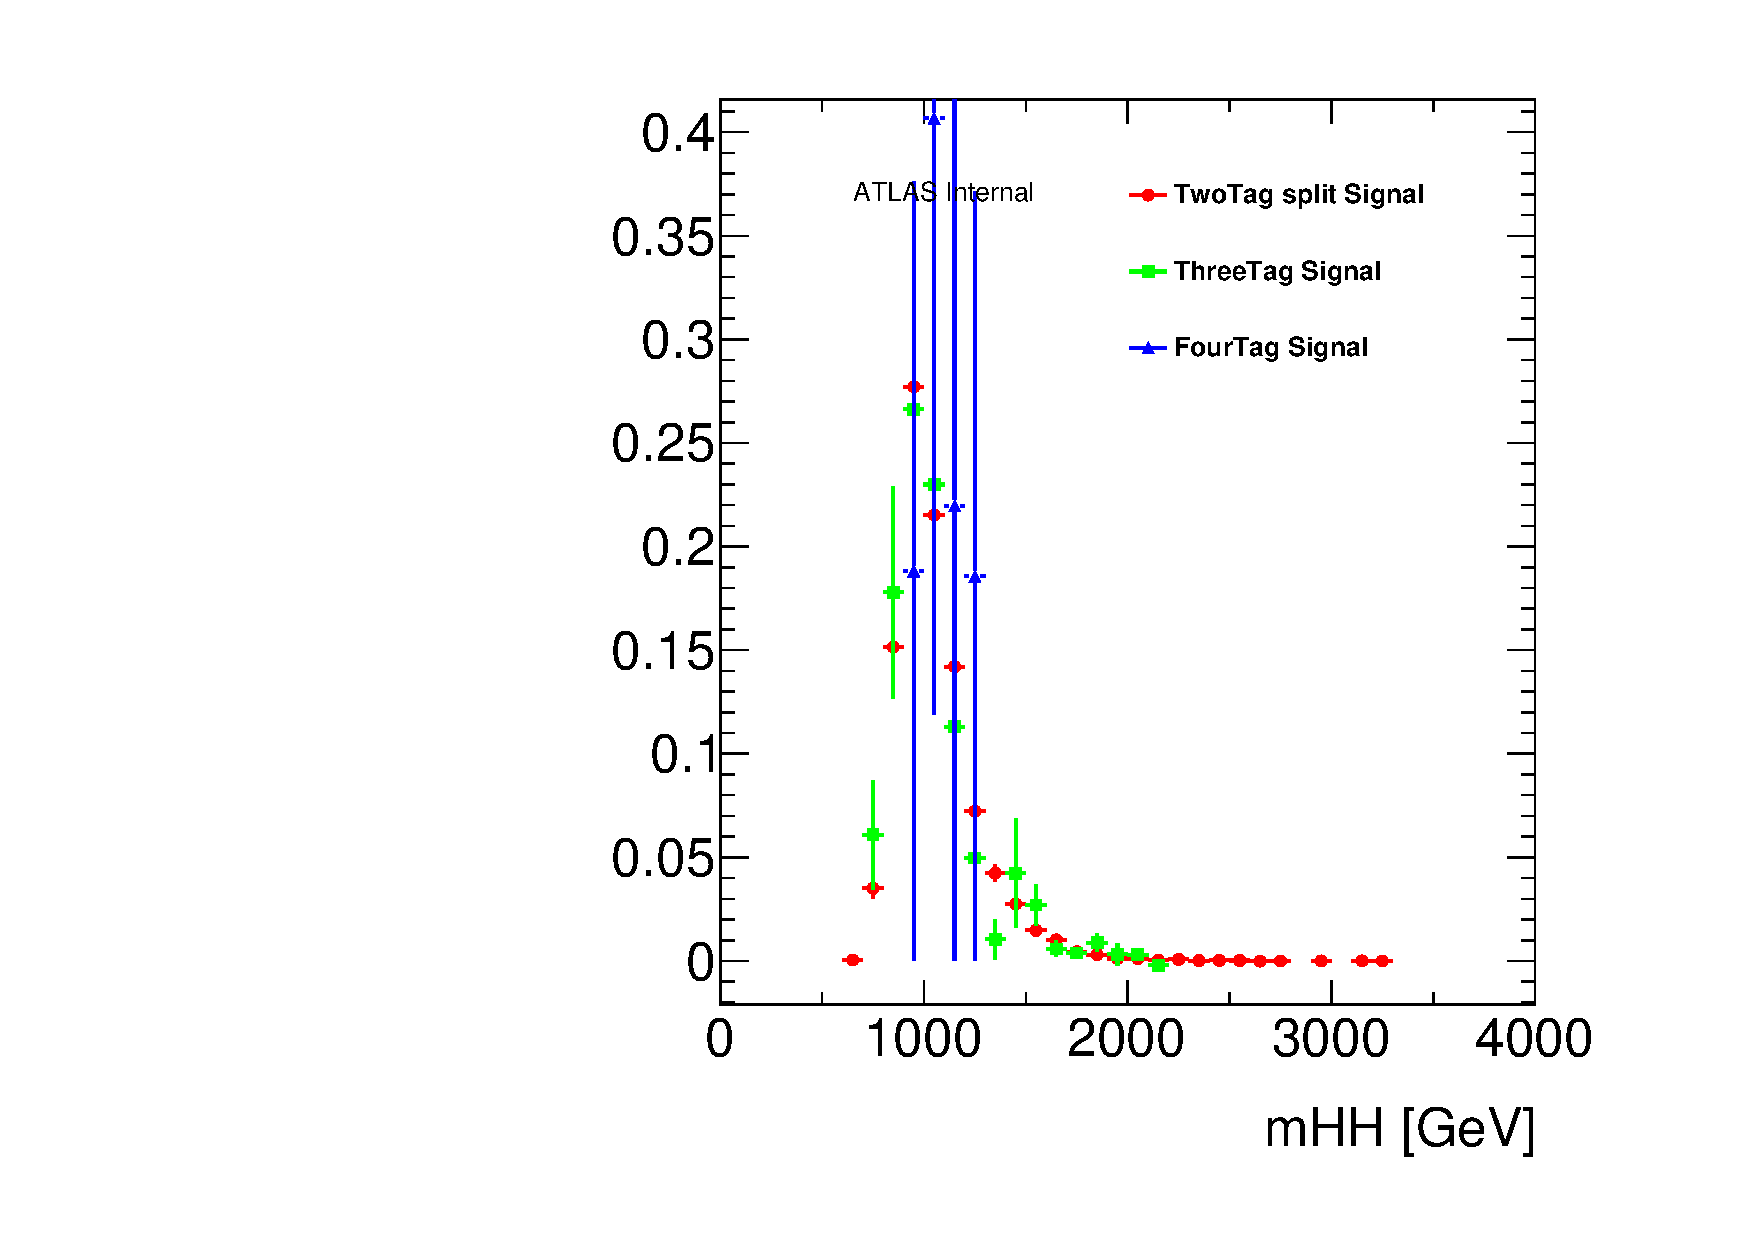
\includegraphics[width=\textwidth,angle=-90]{figures/boosted/Other/ttbar_compare_mHH_l.pdf}
        \caption{Linear scale}
        \label{fig:ttshapeComp_lin}
    \end{subfigure}
    \quad
    \begin{subfigure}[b]{0.45\textwidth}
        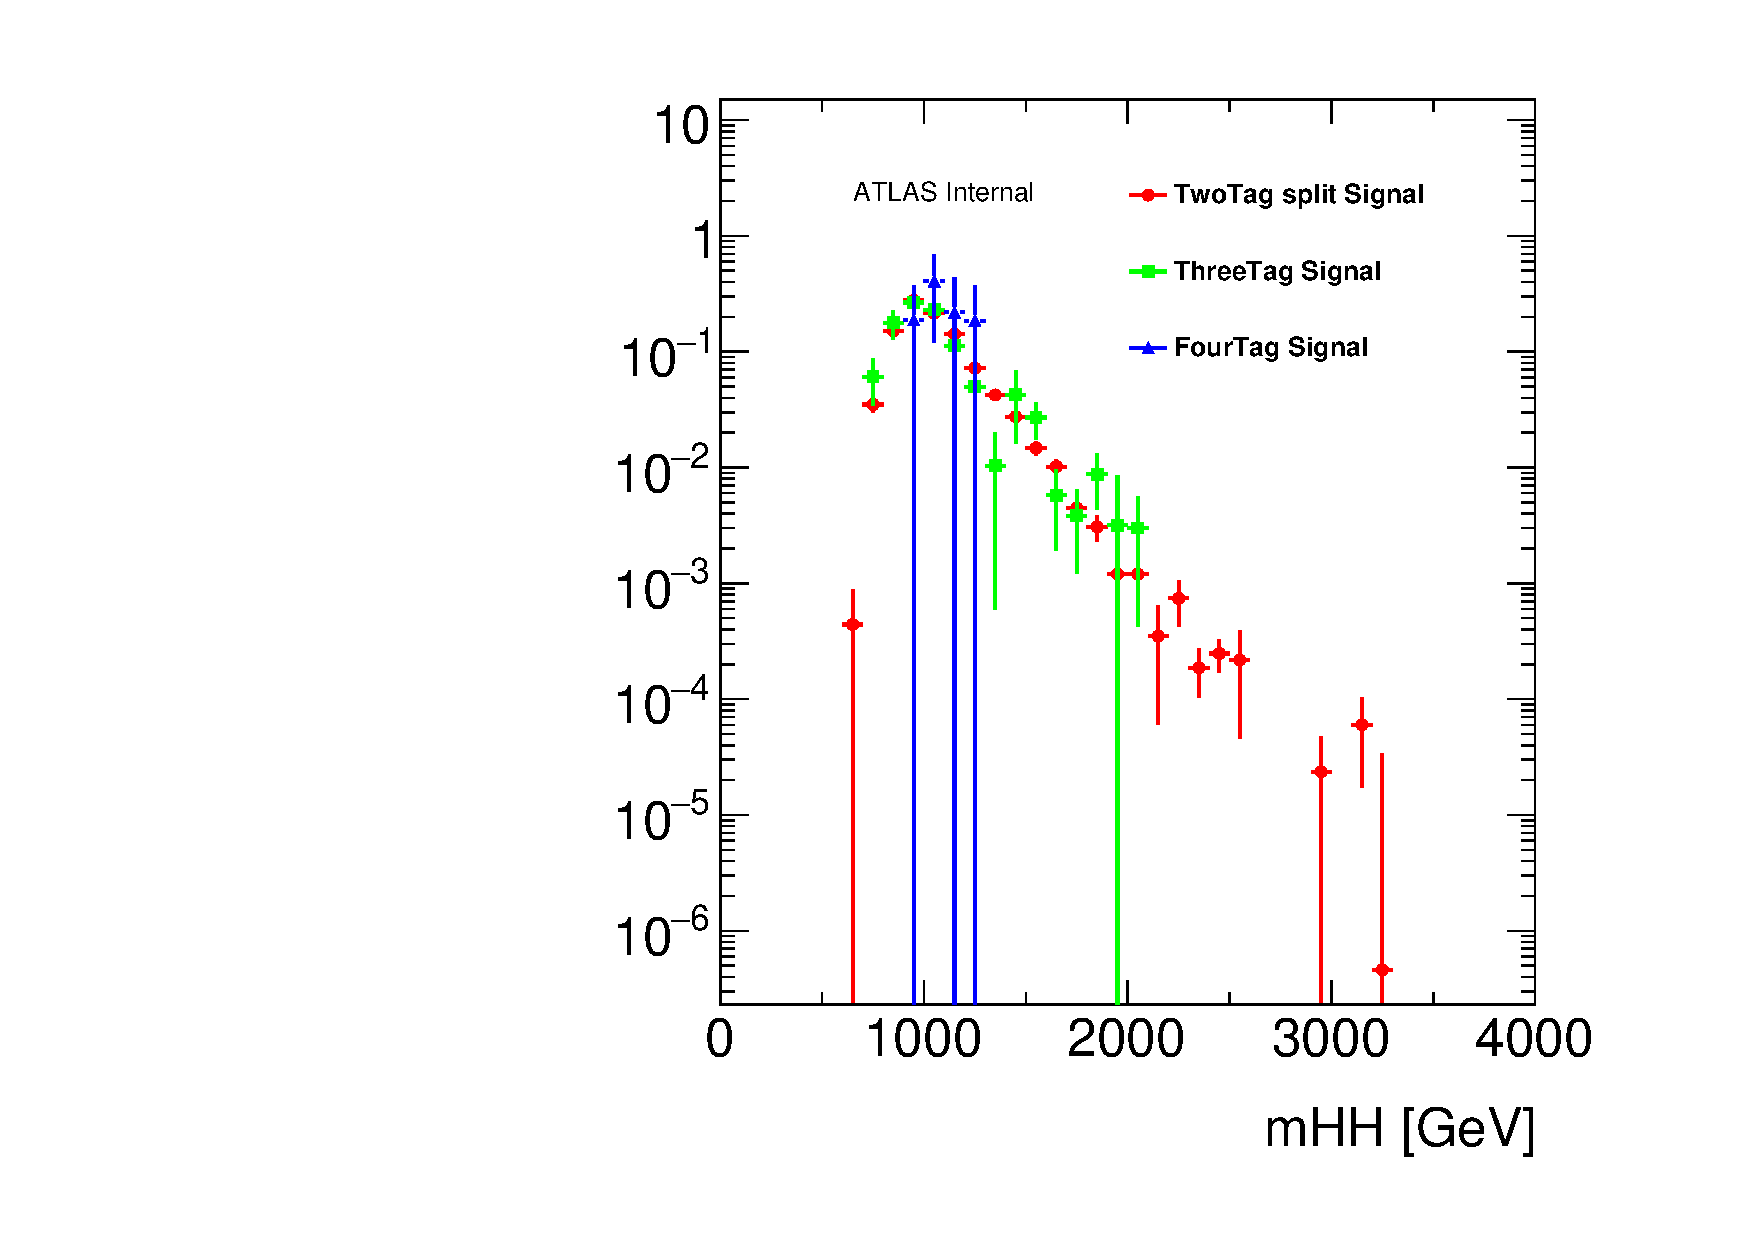
\includegraphics[width=\textwidth,angle=-90]{figures/boosted/Other/ttbar_compare_mHH_l_1.pdf}
        \caption{Log scale}
        \label{fig:ttshapeComp_log}
    \end{subfigure}
   \caption{Normalized of $2bs$, $3b$, and $4b$ \ttbar~ MC \mtwoJ~ distribution in the signal region. The uncertainties are statistical.}
  \label{fig:ttshapeComp}
\end{figure}


%%%%%%%%%%%%%%%%%%%%%%%%%%%%%%%%%%%%%%%%%%%%%%%%%%%%%%%%%%%%%%%%%%%%%%%
%%%%%%%%%%%%%%%%%%%%%%%%%%%%%%%%%%%%%%%%%%%%%%%%%%%%%%%%%%%%%%%%%%%%%%%
%%%  Fitting
%%%%%%%%%%%%%%%%%%%%%%%%%%%%%%%%%%%%%%%%%%%%%%%%%%%%%%%%%%%%%%%%%%%%%%%
%%%%%%%%%%%%%%%%%%%%%%%%%%%%%%%%%%%%%%%%%%%%%%%%%%%%%%%%%%%%%%%%%%%%%%%
\section{Fitting procedure for QCD and \ttbar~ normalization}
\label{sec:ttbarnorm}

\paragraph{}
The number of $4b/3b/2bs$ background events in a given region R (SB / CR / SR) is shown in Equation~\ref{eq:fitparams-4b}, \ref{eq:fitparams-3b} and \ref{eq:fitparams-2bs}:
\begin{eqnarray}
\label{eq:fitparams-4b}
N^{4b\text{-R}}_{\text{bkg}} = \mu_{\text{qcd}}^{4b} N^{2b\text{-R}}_{\text{qcd}} + \alpha_{t\bar{t}}^{4b} N^{4b\text{-R}}_{t\bar{t}} + N^{4b\text{-R}}_{Z+jets};
\quad \mu_{\text{qcd}}^{4b} \sim \frac{N^{4b\text{-SB}}_{\text{qcd}}}{N^{2b\text{-SB}}_{\text{qcd}}}
\\
\label{eq:fitparams-3b}
N^{3b\text{-R}}_{\text{bkg}} = \mu_{\text{qcd}}^{3b\text{-R}} N^{2b\text{-R}}_{\text{qcd}} + \alpha_{t\bar{t}}^{3b} N^{3b\text{-R}}_{t\bar{t}} + N^{3b\text{-R}}_{Z+jets} ;
\quad \mu_{\text{qcd}}^{3b} \sim \frac{N^{3b\text{-SB}}_{\text{qcd}}}{N^{2b\text{-SB}}_{\text{qcd}}}\\
\label{eq:fitparams-2bs}
N^{2bs\text{-R}}_{\text{bkg}} = \mu_{\text{qcd}}^{2bs\text{-R}} N^{1b\text{-R}}_{\text{qcd}} + \alpha_{t\bar{t}}^{2bs} N^{2bs\text{-R}}_{t\bar{t}} + N^{2bs\text{-R}}_{Z+jets};
\quad \mu_{\text{qcd}}^{2bs} \sim \frac{N^{2bs\text{-SB}}_{\text{qcd}}}{N^{1b\text{-SB}}_{\text{qcd}}}
\end{eqnarray} 
\muqcd~ is essentially an estimate of the ratio of the number of QCD events with $4b/3b/2bs$-tagged track jets, to the number of QCD events with $2b/2b/1b$-tagged track jets.
\muqcd~ is assumed to be a constant over SB/CR/SR \mleadJ-\msublJ regions.
Validation of this assumption can be found in Appendix~\ref{AppendixMuqcd}.
\alphatt~, applied after the \ttbar~ MC is scaled to the total integrated luminosity, is a correction to the MC prediction.
\muqcd~ and \alphatt~ are derived in the sideband region.
They are used as multiplicative constants in other regions of the mass plane (i.e. the control region or the signal region).

\paragraph{}
A binned maximum likelihood fit is used to find the values of \muqcd~ and \alphatt~, as well as the correlation between them.
These scaling parameters are determined independently using the same procedure in the $4b/3b/2bs$ sideband regions.
Due to the \pt~ $>450$ \GeV~ cut imposed on the leading large-\R jet, the hadronicly decaying top quark can be fully reconstructed inside the leading large-\R jet. 
The \mleadJ~ from \ttbar~ events has a clean peak around $170$ \GeV~ in the sideband region.
It has the best separation between QCD and \ttbar~ shapes.
Therefore, the fit is performed on the \mleadJ spectrum in the sideband region.

\paragraph{}
Figure~\ref{fig:ttbar-fit} shows the post-fit spectrum of \mleadJ in the $n$-$b$tag sideband regions.
The \mleadJ shapes in data are well modeled by the predicted backgrounds. 
The fitting errors on \muqcd~ and \alphatt~ are applied as systematic uncertainties taking into account their correlation.

\begin{figure}[htbp!]
  \centering
  \captionsetup{justification=centering}
    \hspace{-4cm}
    \begin{subfigure}[b]{0.3\textwidth}
        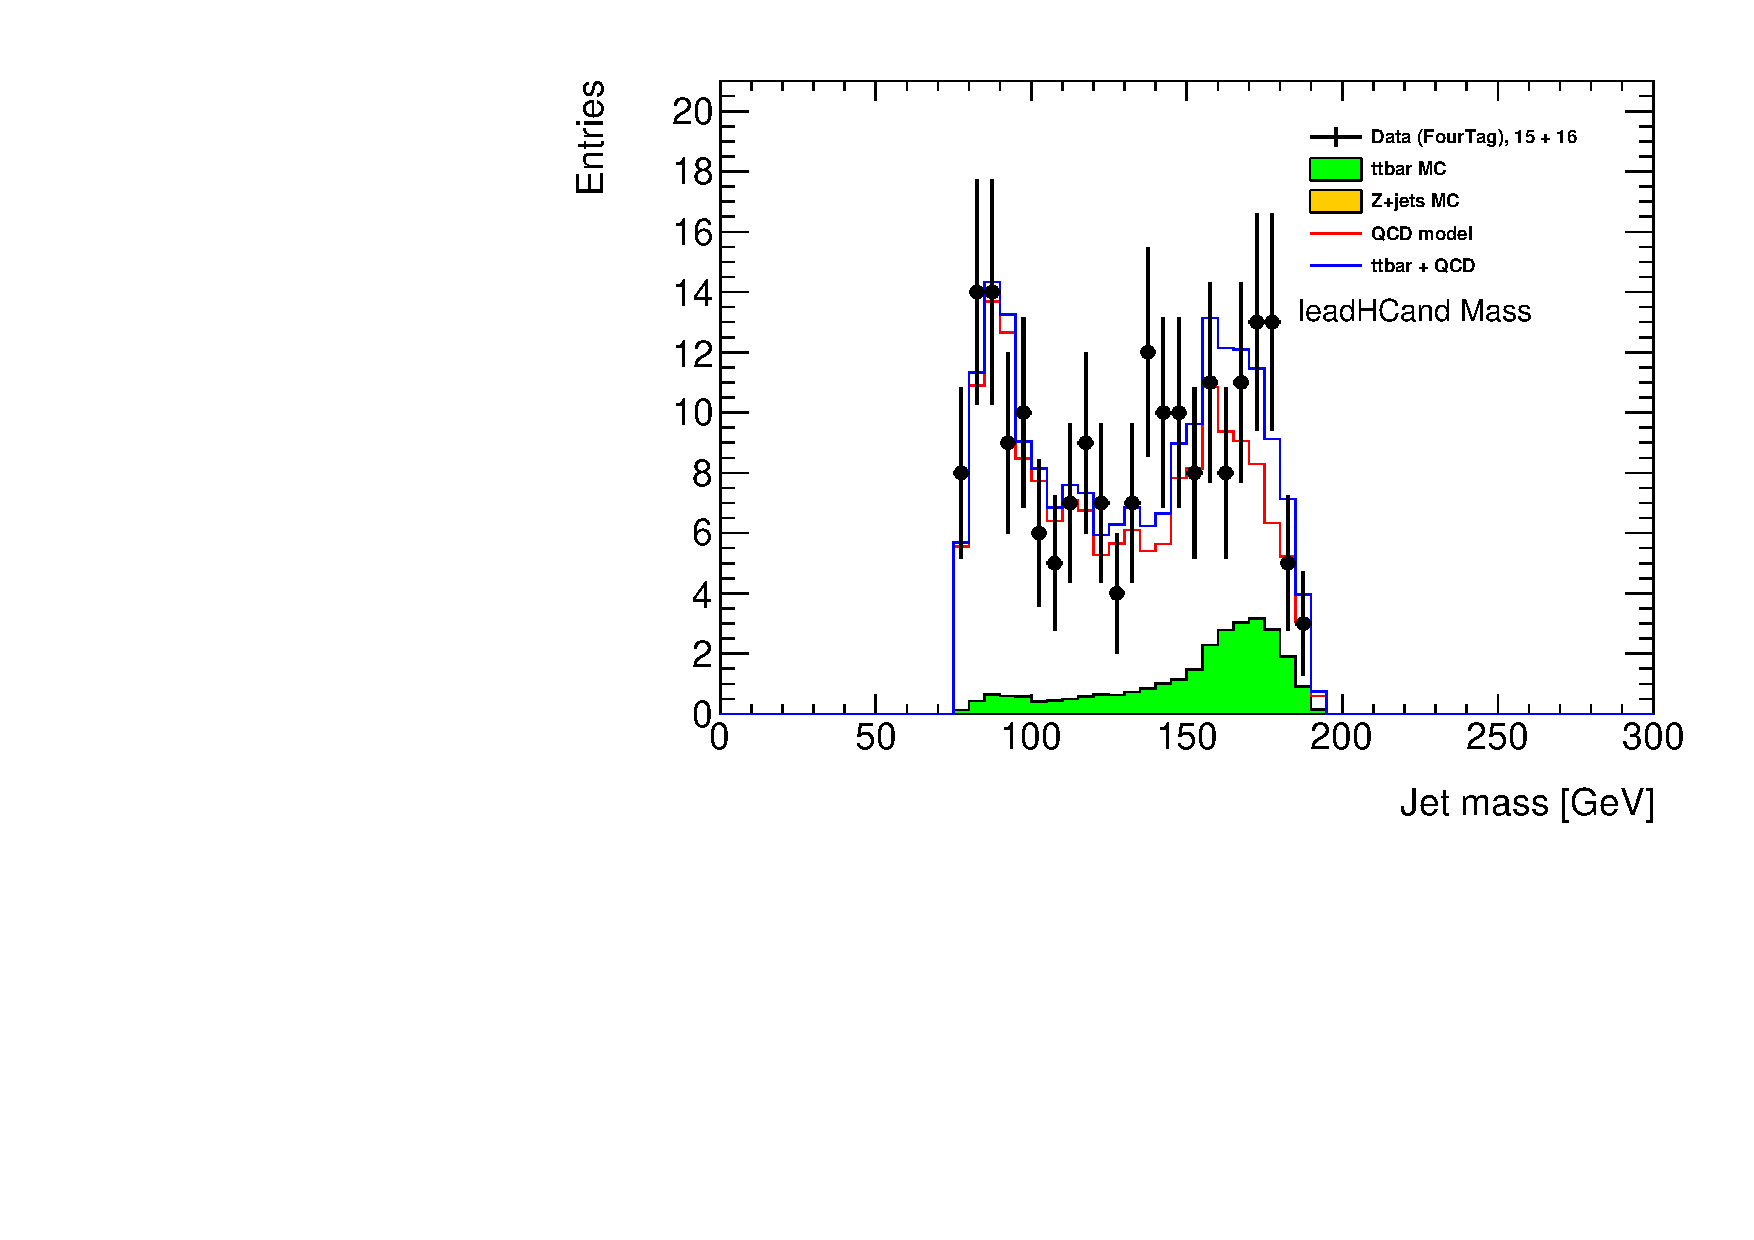
\includegraphics[width=\textwidth,angle=-90]{figures/boosted/Fit/fitNorm_i4.pdf}
        \caption{$4b$ \mleadJ~ fit}
        \label{fig:ttbar-fit-4b}
    \end{subfigure}
    \quad \quad \quad \quad \quad
    \begin{subfigure}[b]{0.3\textwidth}
        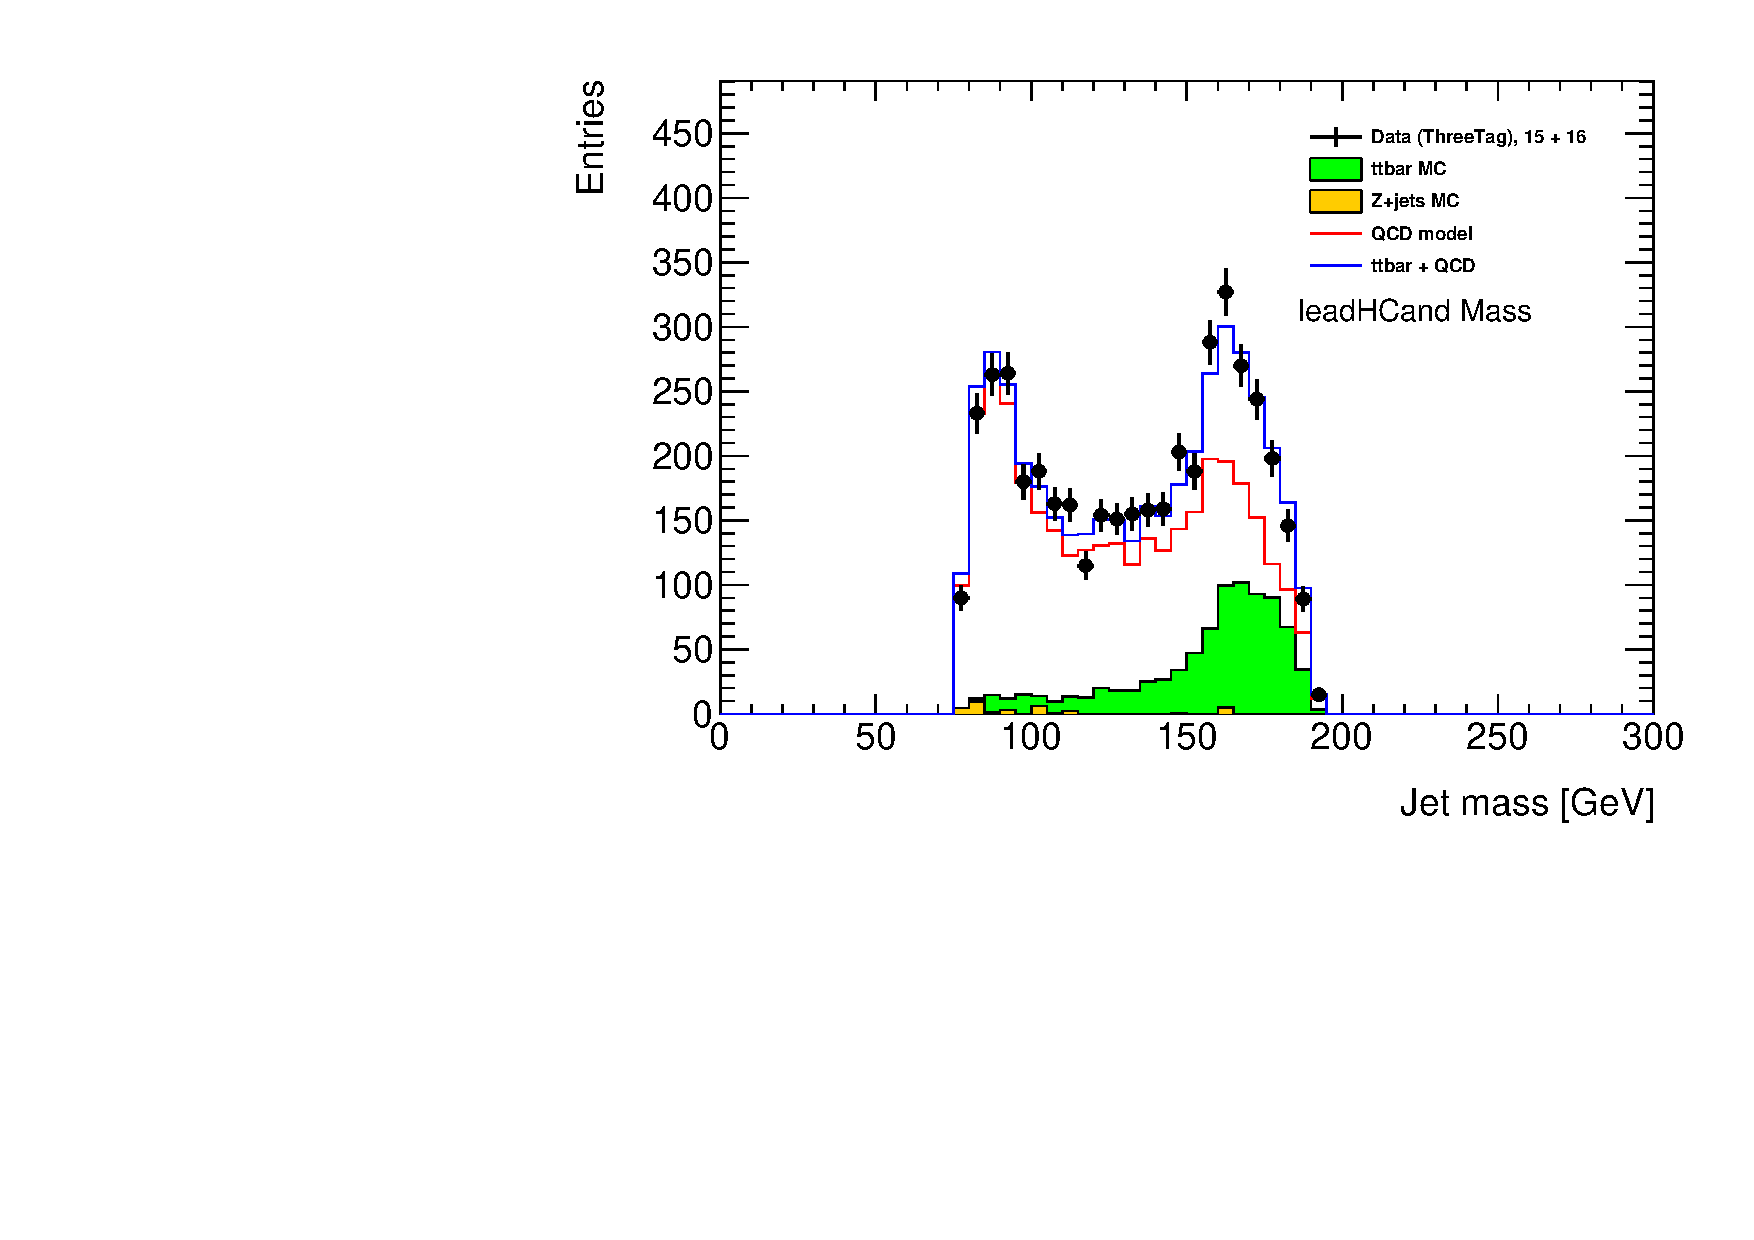
\includegraphics[width=\textwidth,angle=-90]{figures/boosted/Fit/fitNorm_i3.pdf}
        \caption{$3b$ \mleadJ~ fit}
        \label{fig:ttbar-fit-3b}
    \end{subfigure}
    \\
    \hspace{-4cm}
    \begin{subfigure}[b]{0.3\textwidth}
        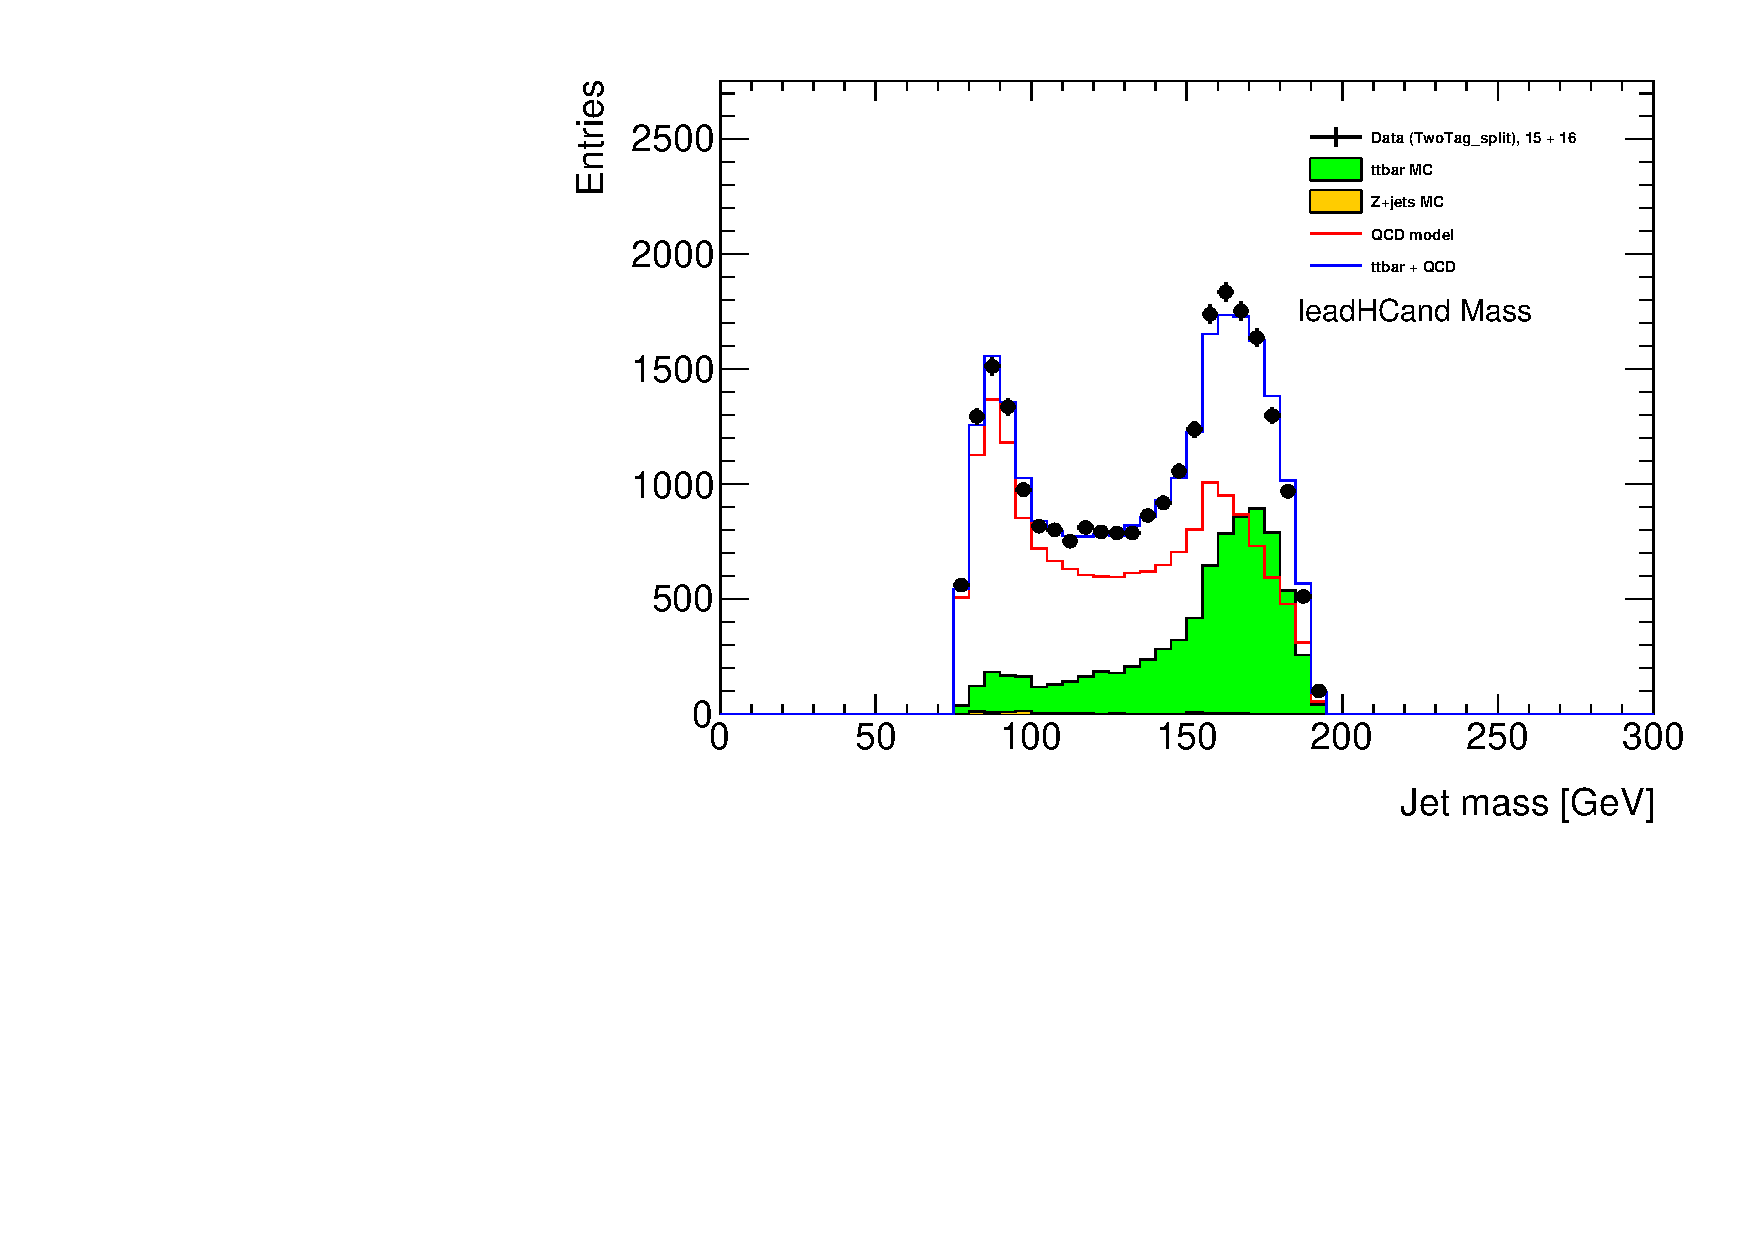
\includegraphics[width=\textwidth,angle=-90]{figures/boosted/Fit/fitNorm_i2s.pdf}
        \caption{$2bs$ \mleadJ~ fit}
        \label{fig:ttbar-fit-2bs}
    \end{subfigure}
   \caption{Simultaneous fit of \muqcd~ and \alphatt~ in $4b$, $3b$ and$2bs$ sideband region using the leading large-\R jet mass.}
  \label{fig:ttbar-fit}
\end{figure}

\paragraph{}
The \ttbar~ MC sample normalization is further corrected from the fitted \alphatt.
At first \alphatt~ is assumed to be $1$.
Once the first fit is done, the QCD background is re-estimated using the updated $2bs$ \alphatt~value, which has the smallest uncertainty.
Then the fit is repeated until the change in \alphatt~ is less than $0.01$.
This iterative procedure helps correct the \alphatt~ bias in the data driven QCD template.

\paragraph{}
The values of \muqcd~ and \alphatt~ estimated by the fits in the $4b/3b/2bs$ sideband regions can be found in Table~\ref{tab:bkgfit_prereweight}, along with the correlation $\rho(\mu_{qcd},\alpha_{t\bar{t}}) = \frac{Cov(\rm \mu_{qcd},\rm \alpha_{tt})}{\rm \sigma_{\mu_{qcd}} \rm \sigma_{\alpha_{tt}} }$. 
\muqcd~ and \alphatt~  are approximately $70\%$ negatively correlated, due to the two components fit nature.
This negative correlation leads to a smaller total normalization uncertainty.

\begin{table}[htbp!]
\begin{center}
\caption{Background scaling parameters (\muqcd and \alphatt) estimated from fits to the \mleadJ distributions in $4b/3b/2bs$ sideband regions pre-reweighting. $\rho(\mu_{qcd},\alpha_{t\bar{t}}) = \frac{Cov(\rm \mu_{qcd},\rm \alpha_{\rm tt})}{\rm \sigma_{\mu_{qcd}} \rm \sigma_{\rm \alpha_{ tt}} }$.}
\begin{footnotesize} 
\begin{tabular}{c|c|c|c} 
Sample & $\mu_{qcd}$ & $\alpha_{t\bar{t}}$ & $\rho(\mu_{qcd}, \alpha_{t\bar{t}})$ \\ 
\hline\hline 
FourTag & 0.033987 $\pm$ 0.0043057 & 1.01697 $\pm$ 0.58642 & -0.76397\\
ThreeTag & 0.16247 $\pm$ 0.0041713 & 0.86508 $\pm$ 0.069019 & -0.6778\\
TwoTag split & 0.066713 $\pm$ 0.00091137 & 1.03747 $\pm$ 0.026199 & -0.74785\\
\hline\hline 
\end{tabular} 
\end{footnotesize} 
\newline 

\label{tab:bkgfit_prereweight}
\end{center}
\end{table}


%%%%%%%%%%%%%%%%%%%%%%%%%%%%%%%%%%%%%%%%%%%%%%%%%%%%%%%%%%%%%%%%%%%%%%%
%%%%%%%%%%%%%%%%%%%%%%%%%%%%%%%%%%%%%%%%%%%%%%%%%%%%%%%%%%%%%%%%%%%%%%%
%%%  Reweighting
%%%%%%%%%%%%%%%%%%%%%%%%%%%%%%%%%%%%%%%%%%%%%%%%%%%%%%%%%%%%%%%%%%%%%%%
%%%%%%%%%%%%%%%%%%%%%%%%%%%%%%%%%%%%%%%%%%%%%%%%%%%%%%%%%%%%%%%%%%%%%%%

\section{QCD reweighting}
\label{sec:boosted-reweight}

\paragraph{}
This is the most time consuming part of this analysis. 
More supporting plots are shown in Appendix~\ref{AppendixRW}.
It is important to model the QCD background as good as possible in all regions of the analysis.
Using the $1/2b$ region to model the $2bs/3b/4b$ regions can introduce discrepancies in the modeling of the estimated QCD background versus the data. 
These discrepancies arise from the non-trivial effect that $b$-tagging has on jet kinematics.

\begin{figure}[htbp!]
  \centering
  \captionsetup{justification=centering}
    \begin{subfigure}[b]{0.4\textwidth}
        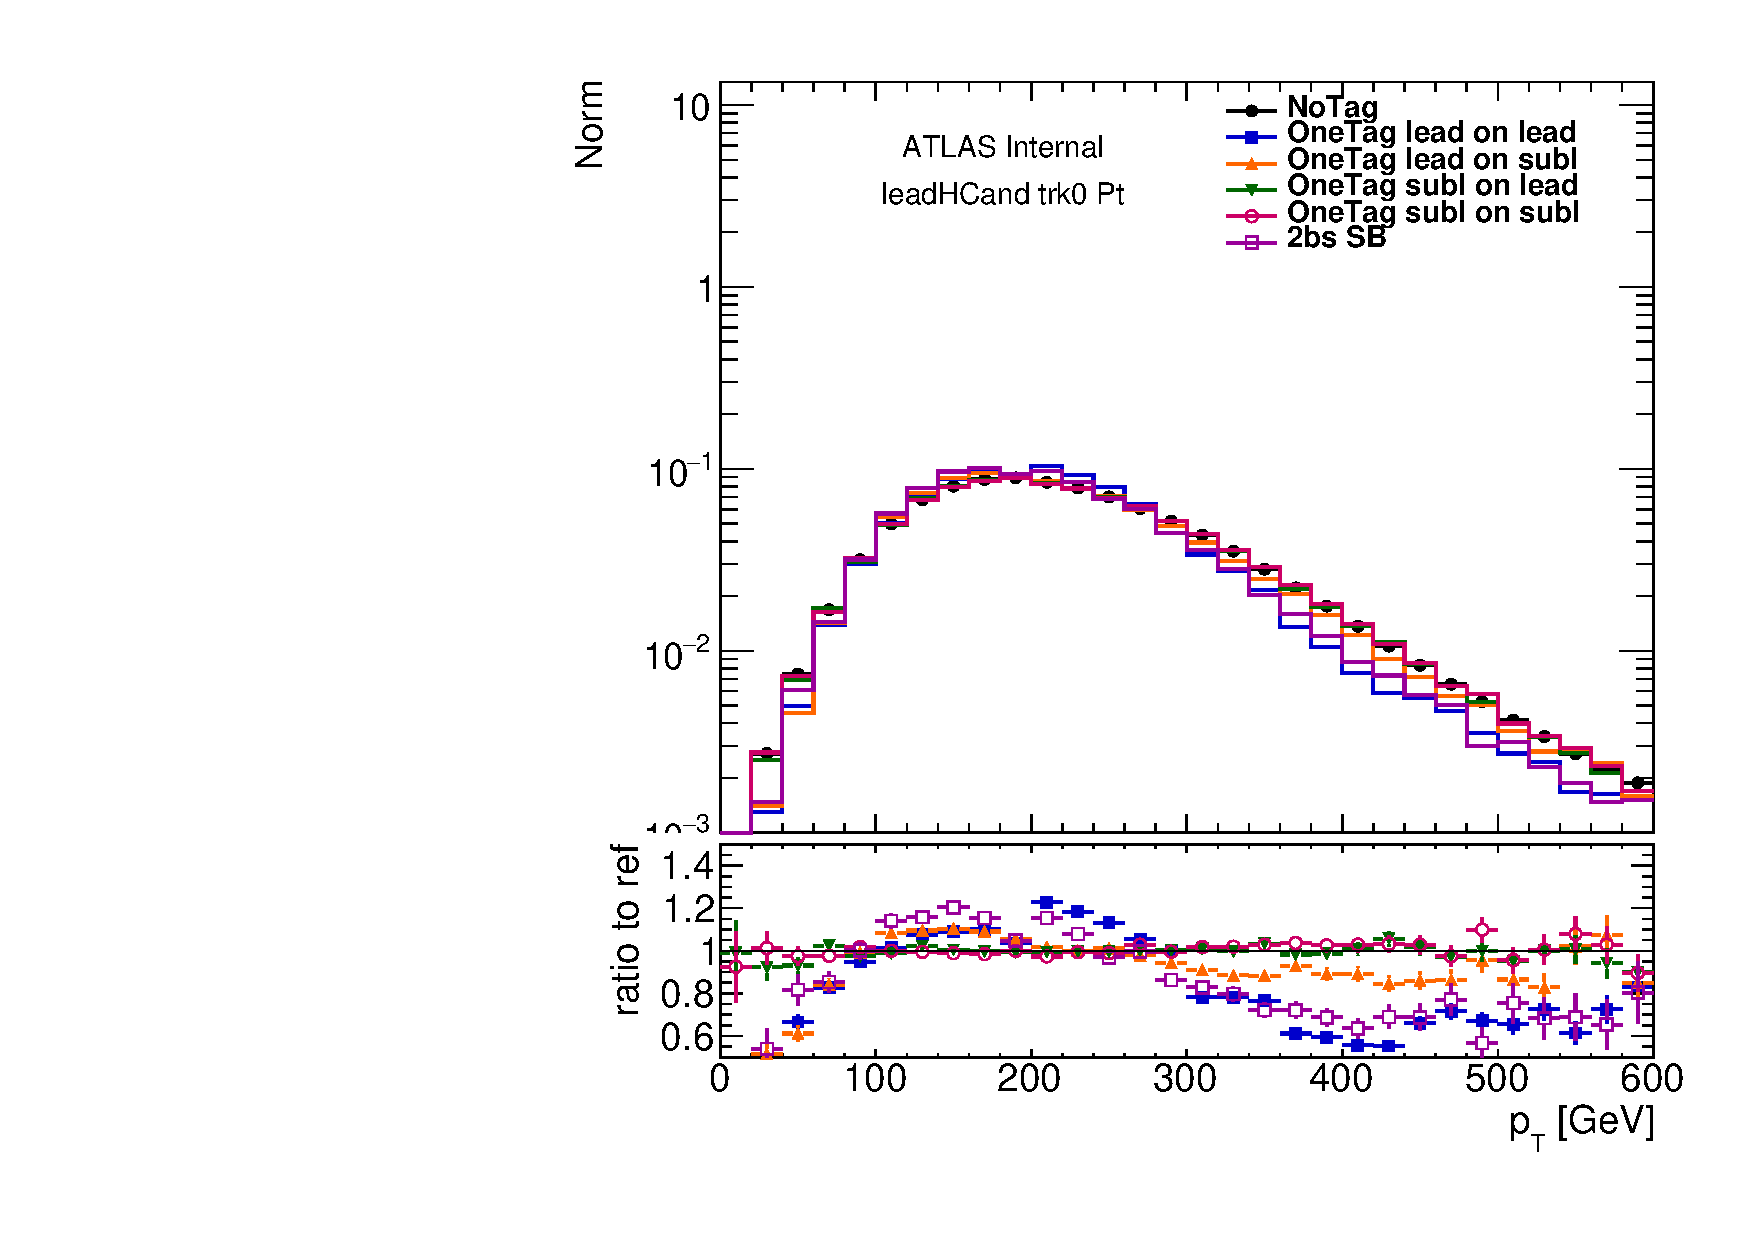
\includegraphics[width=\textwidth,angle=-90]{figures/boosted/Prereweight/2bs_directcompare_leadHCand_trk0_Pt_1.pdf}
        \caption{leading large-\R jet's leading track jet \pt}
        \label{fig:rw-2bs-comp-lead0}
    \end{subfigure}
    \quad \quad 
    \begin{subfigure}[b]{0.4\textwidth}
        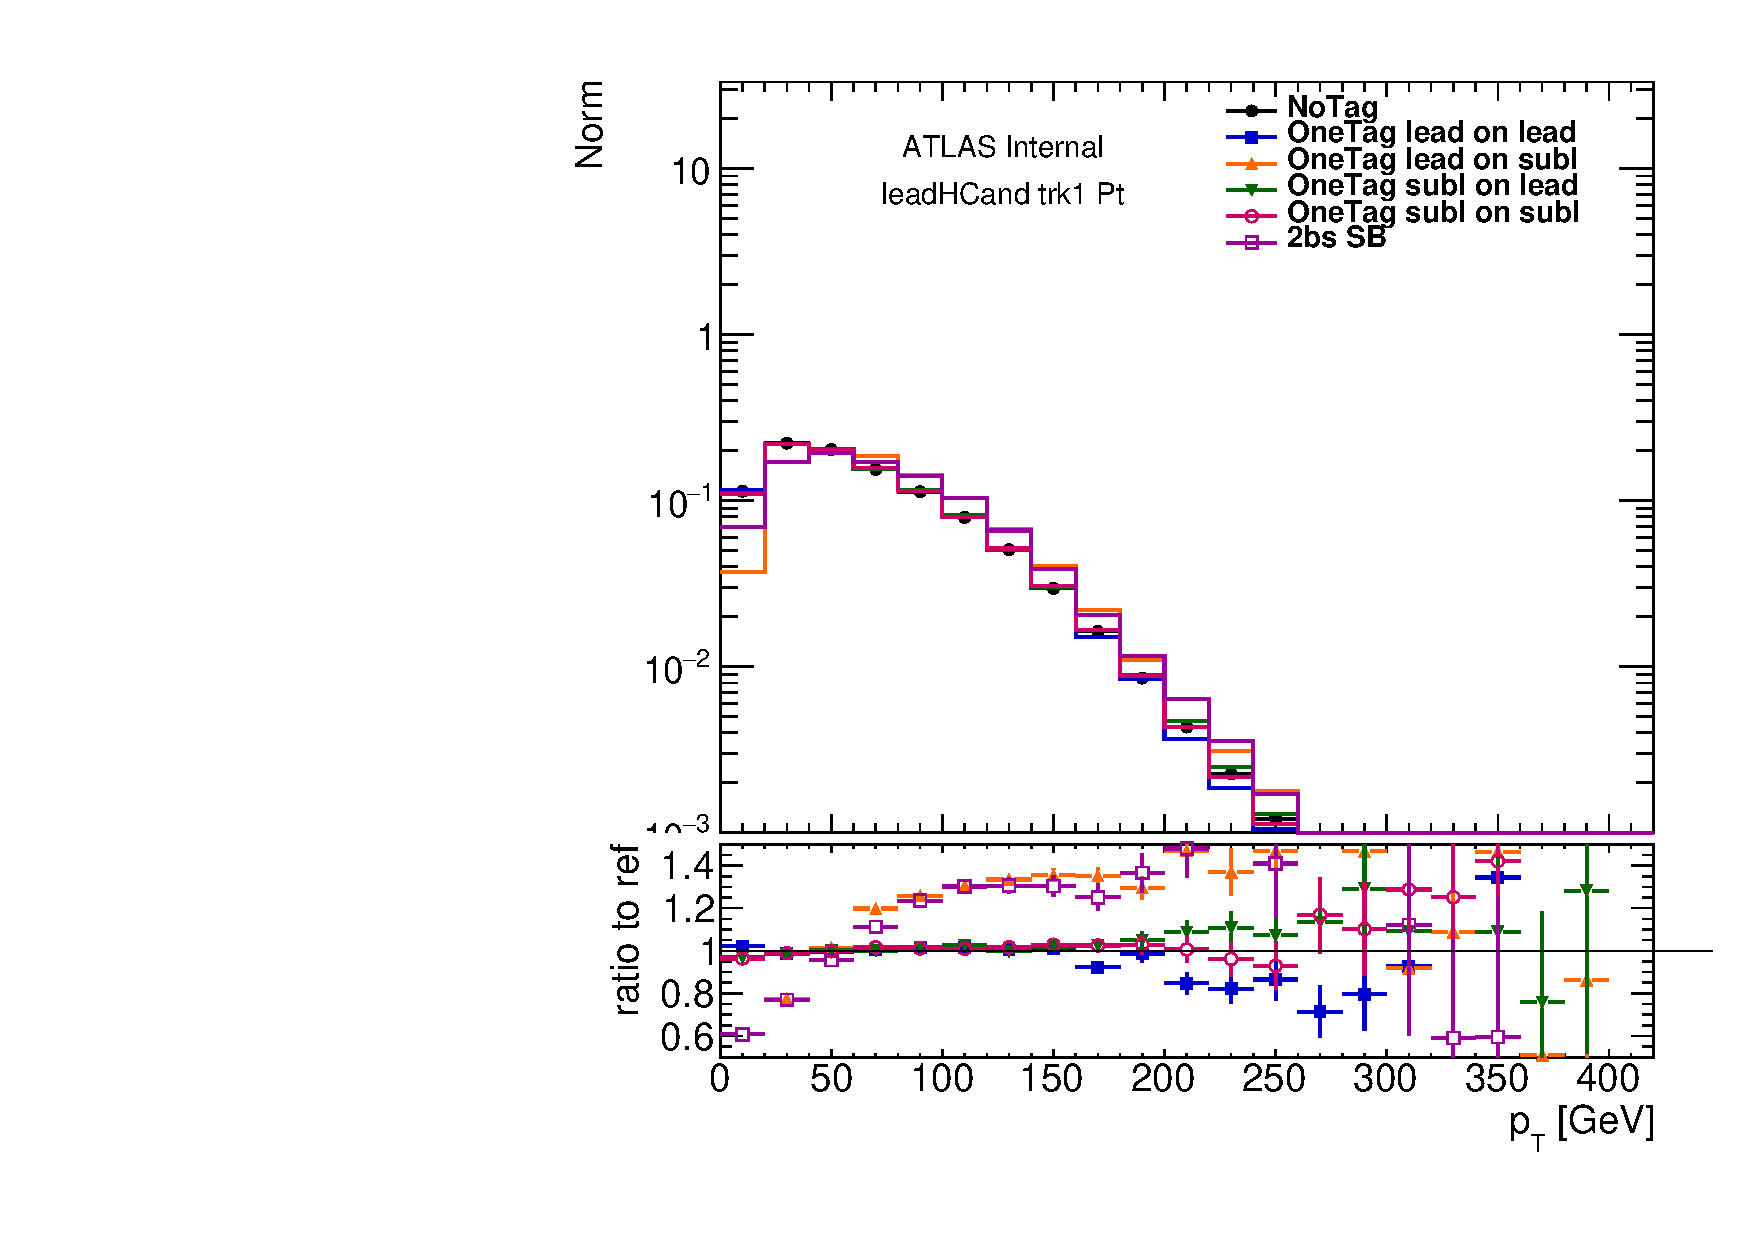
\includegraphics[width=\textwidth,angle=-90]{figures/boosted/Prereweight/2bs_directcompare_leadHCand_trk1_Pt_1.pdf}
        \caption{leading large-\R jet's subleading track jet \pt}
        \label{fig:rw-2bs-comp-lead1}
    \end{subfigure} \\ 
    \begin{subfigure}[b]{0.4\textwidth}
        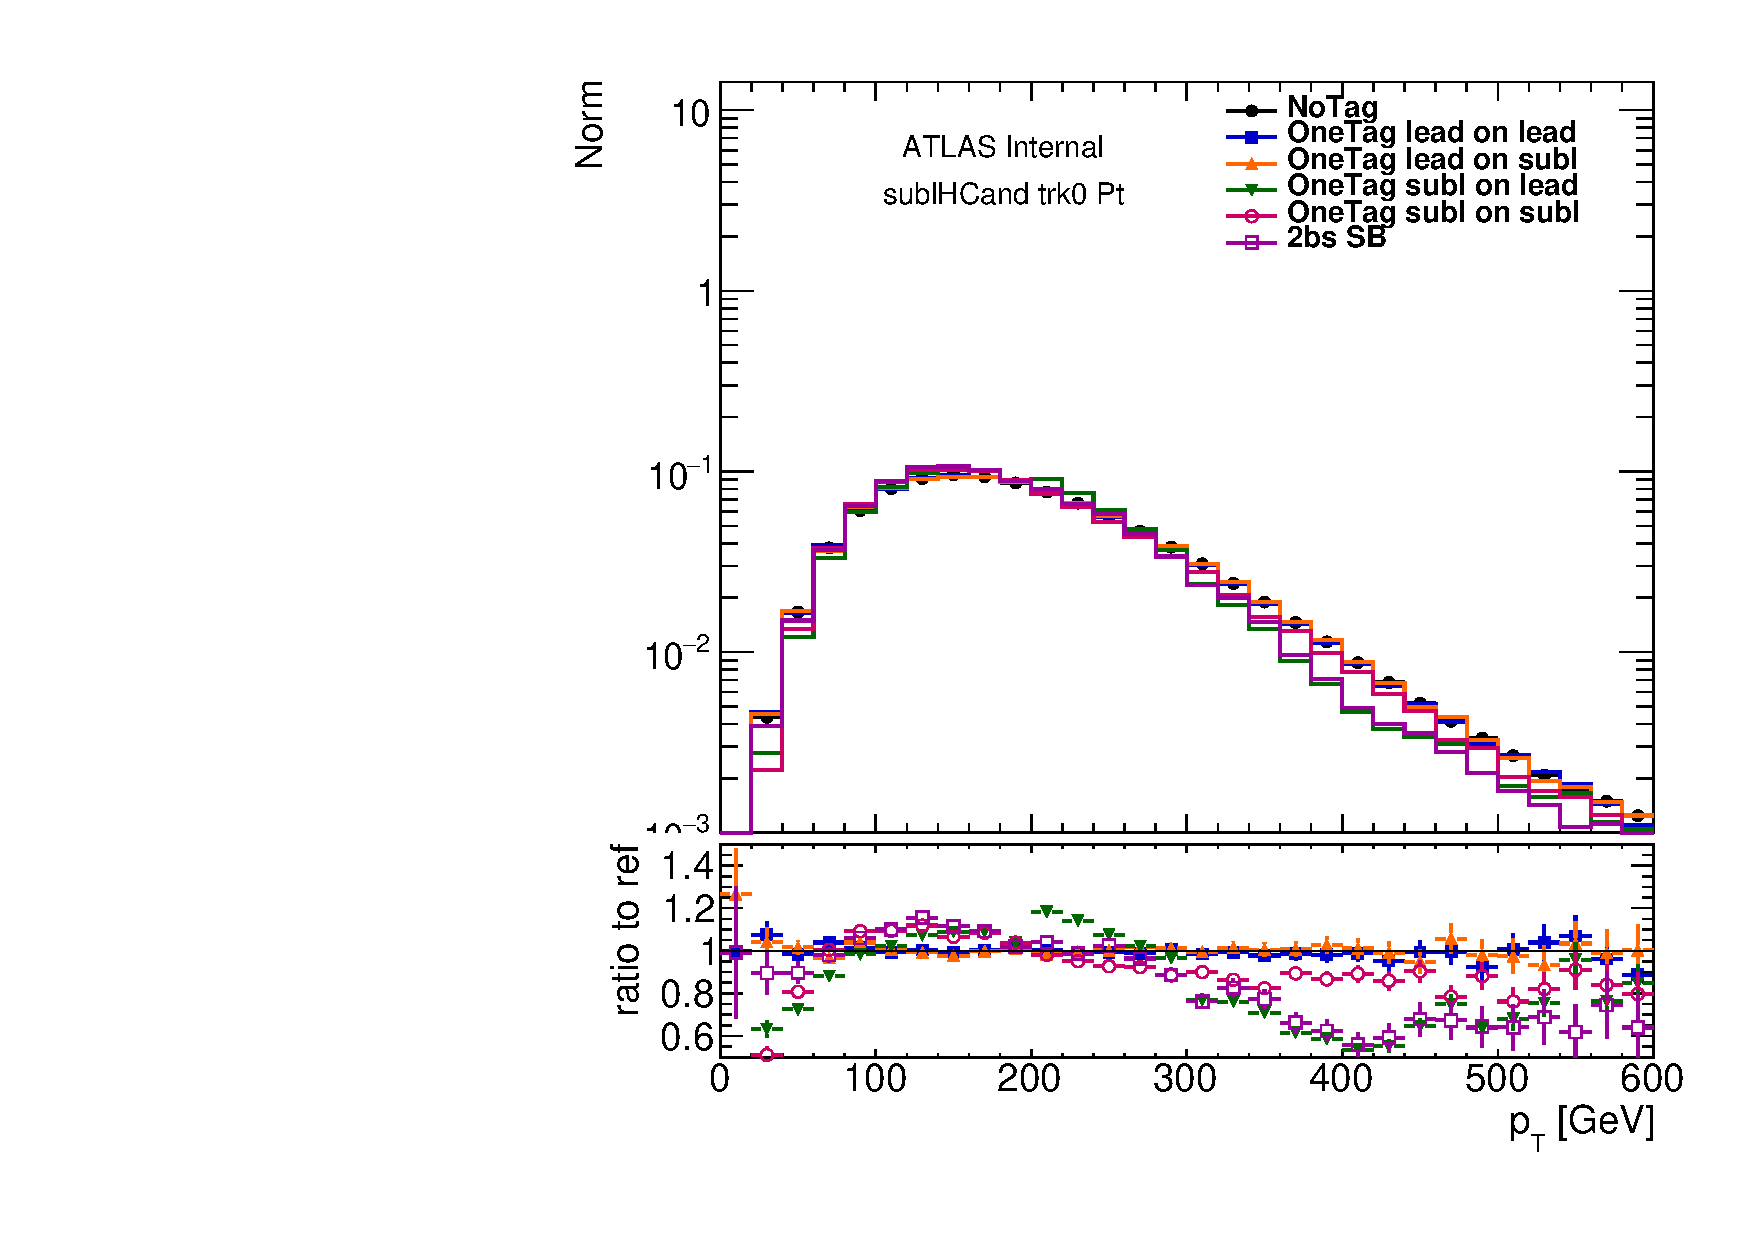
\includegraphics[width=\textwidth,angle=-90]{figures/boosted/Prereweight/2bs_directcompare_sublHCand_trk0_Pt_1.pdf}
        \caption{subleading large-\R jet's leading track jet \pt}
        \label{fig:rw-2bs-comp-subl0}
    \end{subfigure}
    \quad \quad 
    \begin{subfigure}[b]{0.4\textwidth}
        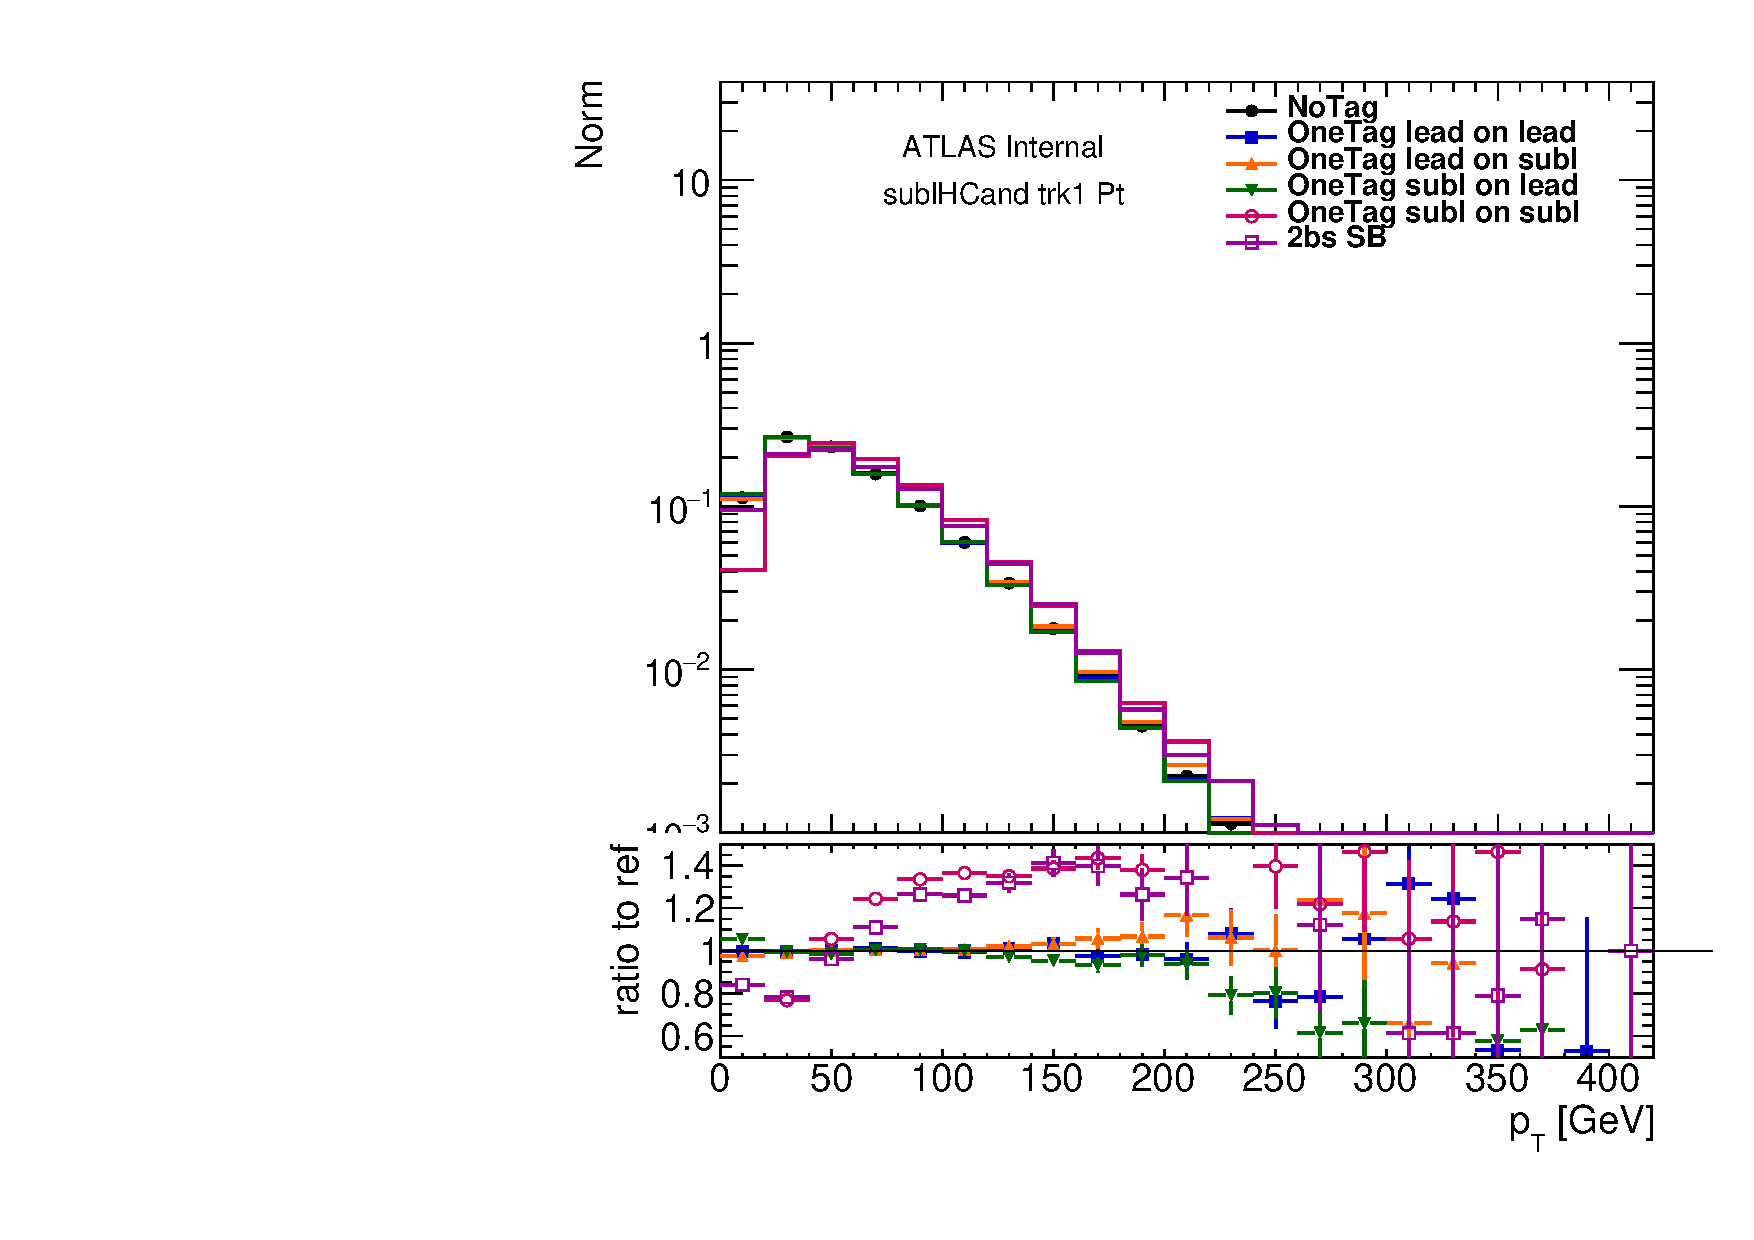
\includegraphics[width=\textwidth,angle=-90]{figures/boosted/Prereweight/2bs_directcompare_sublHCand_trk1_Pt_1.pdf}
        \caption{subleading large-\R jet's subleading track jet \pt}
        \label{fig:rw-2bs-comp-subl1}
    \end{subfigure} \\ 
   \caption{
   Comparison of track jet \pt distributions in different $b$-tag regions.Shown in the plot are data, inclusive of SB/CR/SR regions for $0b$ and $1b$, and only the SB region for $2bs$. At the bottom plot, all the ratios are taken with respect to the $0b$ tagged distribution.}
  \label{fig:rw-2bs-comp}
\end{figure}

\paragraph{}
In order to account for the $b$-tagging effect, a reweighting on the $1/2b$ data is adopted. 
The goal is to reweigh the non $b$-tagged Higgs candidate to have kinematic distributions just like a $b$-tagged Higgs candidate. 
This is motivated by Figure~\ref{fig:rw-2bs-comp}.
$0b$, $1b$ and $2bs$ data are compared.
Except $2bs$ is only showing SB region, $0b$ and $1b$s are inclusive SB$+$CR$+$SR regions.
$1b$ sample is further split into four subcategories, depending on which track jet gets $b$ tagged:
\begin{itemize}
\item ``OneTag lead on lead'' means the only $b$-tagged track jet is the leading track jet of the leading Higgs candidate;
\item ``OneTag lead on subl'' means the only $b$-tagged track jet is the subleading track jet of the leading Higgs candidate;
\item ``OneTag subl on lead'' means the only $b$-tagged track jet is the leading track jet of the subleading Higgs candidate; 
\item ``OneTag subl on subl'' means the only $b$-tagged track jet is the subleading track jet of the subleading Higgs candidate;
\end{itemize}
The figure shows that $2bs$ has very similar track jet \pt~ distributions as the $1b$ sample with a $b$-tagged track jet.
It also shows that in the $1b$ sample, the track jet \pt~ distribution in the non $b$-tagged Higgs candidate behaves like the $0b$ sample's track jet \pt~ distribution.
This result motivates the reweighting method.

\paragraph{}
To avoid potential biases in the final distributions used for the analysis, this reweighting technique is applied to the $1/2b$ data only. 
Since each signal region is modeled by a different $1/2b$ tag category, the reweighting procedure is the same for the three different channels. 
The $2b$ sample is already split into separate parts for $3b$ and $4b$ estimations, as described in section \ref{sec:boosted-qcd}.

\paragraph{}
For $2bs$, the $1b$ non-$b$tagged Higgs candidate is reweighted to be like a $1b$ tagged Higgs candidate; for $3b$, the $2b$ non-$b$tagged Higgs candidate is reweighted to be like a $1b$ tagged Higgs candidate; for $4b$, the $2b$ non-$b$tagged Higgs candidate is reweighted to be like a $2b$ tagged Higgs candidate.
For each category, the events are split into two orthogonal subgroups, based on whether leading/subleading Higgs candidate is $b$-tagged.
Each event gets a weight, such that the reweighted untagged Higgs candidate's distributions agree with the corresponding $b$-tagged Higgs candidate's.

\paragraph{}
One natural choice of reweighting variable is the \pt~ of the track jets in the event, since $b$-tagging efficiency and $b$-tagging fake rate have a strong track jet \pt~ dependence. 
Also, large-\R jet \pt~ is reweighted to account for the difference from light/$c$/$b$ quarks composition in QCD events at different energy scales.
The three reweighted variables are the leading large-\R jet \pt~, leading large-\R jet leading track jet \pt~ and subleading large-\R jet leading track jet \pt~.

\paragraph{}
The each reweighting iteration is described below:
\begin{itemize}
\item Subtract $1/2b$ \ttbar and $Z+$jets samples in the SB + CR + SR regions from the $1/2b$ tag data in the SB + CR + SR regions to get the $1/2b$ QCD inclusive estimate. Weights from all previous iterations, if applicable, are all applied.
\item Separate the $1/2b$ sample into two parts: A. that has the $b$-tagged Higgs is the leading \pt Higgs candidate, and B. that the $b$-tagged Higgs is the subleading \pt Higgs candidate.
\item For each variable, i.e. the large-\R jet $p_{T}$: normalize sample A to sample B's total number of events, take the ratio of sample A's distribution over sample B's distribution, and fit the ratio with a smooth spline function. (TSpline3)
\item Use this spline function to extract reweighting values for each variable that is considered. Then, the difference from one is scaled by $0.75$ to get a new weight. This accounts for over correlation by the spline and accelerates convergence.
\item For each event, all the three weights from three variables are multiplied together to get a data event weight. Another constraint is applied, such that each event's total reweighting value is constrained to be within a $0.05$ to $10$ range compared to $1$. This avoids over corrections.
\end{itemize}
A total of ten iterations are used to stabilize the reweighting. 
The reweighting is almost converging after three iterations.
The reweighting value for each variable is also constrained to be within a $-30\%$ to $+40\%$ range compared to one, to avoid over corrections and failed fit situations.

\begin{table}[htbp!]
\begin{center}
\caption{Background scaling parameters (\muqcd and \alphatt) estimated from fits to the \mleadJ distributions in $4b/3b/2bs$ sideband regions post reweighting. $\rho(\mu_{qcd},\alpha_{t\bar{t}}) = \frac{Cov(\rm \mu_{qcd},\rm \alpha_{\rm t\bar{t}})}{\rm \sigma_{\mu_{qcd}} \rm \sigma_{\alpha_{\rm t\bar{t}}} }$.}
\begin{footnotesize} 
\begin{tabular}{c|c|c|c} 
Sample & $\mu_{qcd}$ & $\alpha_{t\bar{t}}$ & $\rho(\mu_{qcd}, \alpha_{t\bar{t}})$ \\ 
\hline\hline 
FourTag & 0.033167 $\pm$ 0.0042799 & 0.89136 $\pm$ 0.59866 & -0.7846\\
ThreeTag & 0.16256 $\pm$ 0.0043405 & 0.79989 $\pm$ 0.073276 & -0.72029\\
TwoTag split & 0.062726 $\pm$ 0.00057307 & 0.98637 $\pm$ 0.018582 & -0.4698\\
\hline\hline 
\end{tabular} 
\end{footnotesize} 
\newline 

\label{tab:bkgfit}
\end{center}
\end{table}

\paragraph{}
At the end of reweighting, the \muqcd and \alphatt is re-evaluated. The estimated \muqcd and \alphatt values before reweighting can be found in Table~\ref{tab:bkgfit}. 
The values are statistically consistent with the values in Table~\ref{tab:bkgfit_prereweight}.


%For reweighting method comparisons and validations in data and Dijet MC, see Appendix~\ref{app:reweightstudy}.
%For the distribution of weights and the weight as a function of different kinematic ranges, see Appendix~\ref{app:reweight-dist}.

%%%%%%%%%%%%%%%%%%%%%%%%%%%%%%%%%%%%%%%%%%%%%%%%%%%%%%%%%%%%%%%%%%%%%%%
%%%%%%%%%%%%%%%%%%%%%%%%%%%%%%%%%%%%%%%%%%%%%%%%%%%%%%%%%%%%%%%%%%%%%%%
%%%  SB plots
%%%%%%%%%%%%%%%%%%%%%%%%%%%%%%%%%%%%%%%%%%%%%%%%%%%%%%%%%%%%%%%%%%%%%%%
%%%%%%%%%%%%%%%%%%%%%%%%%%%%%%%%%%%%%%%%%%%%%%%%%%%%%%%%%%%%%%%%%%%%%%%
\section{\mtwoJ~ in the sideband region}
\label{sec:boosted-sb}

\paragraph{}
Figure~\ref{fig:boosted-sb-mjj} shows comparisons of the predicted \mtwoJ~background distributions to those observed in the data in the sideband region.
The predicted background and observed distributions are in agreement, with no significant excess.
Other sideband region distributions are shown in Appendix~\ref{AppendixSB}.

\begin{figure}[htbp!]
\begin{center}
 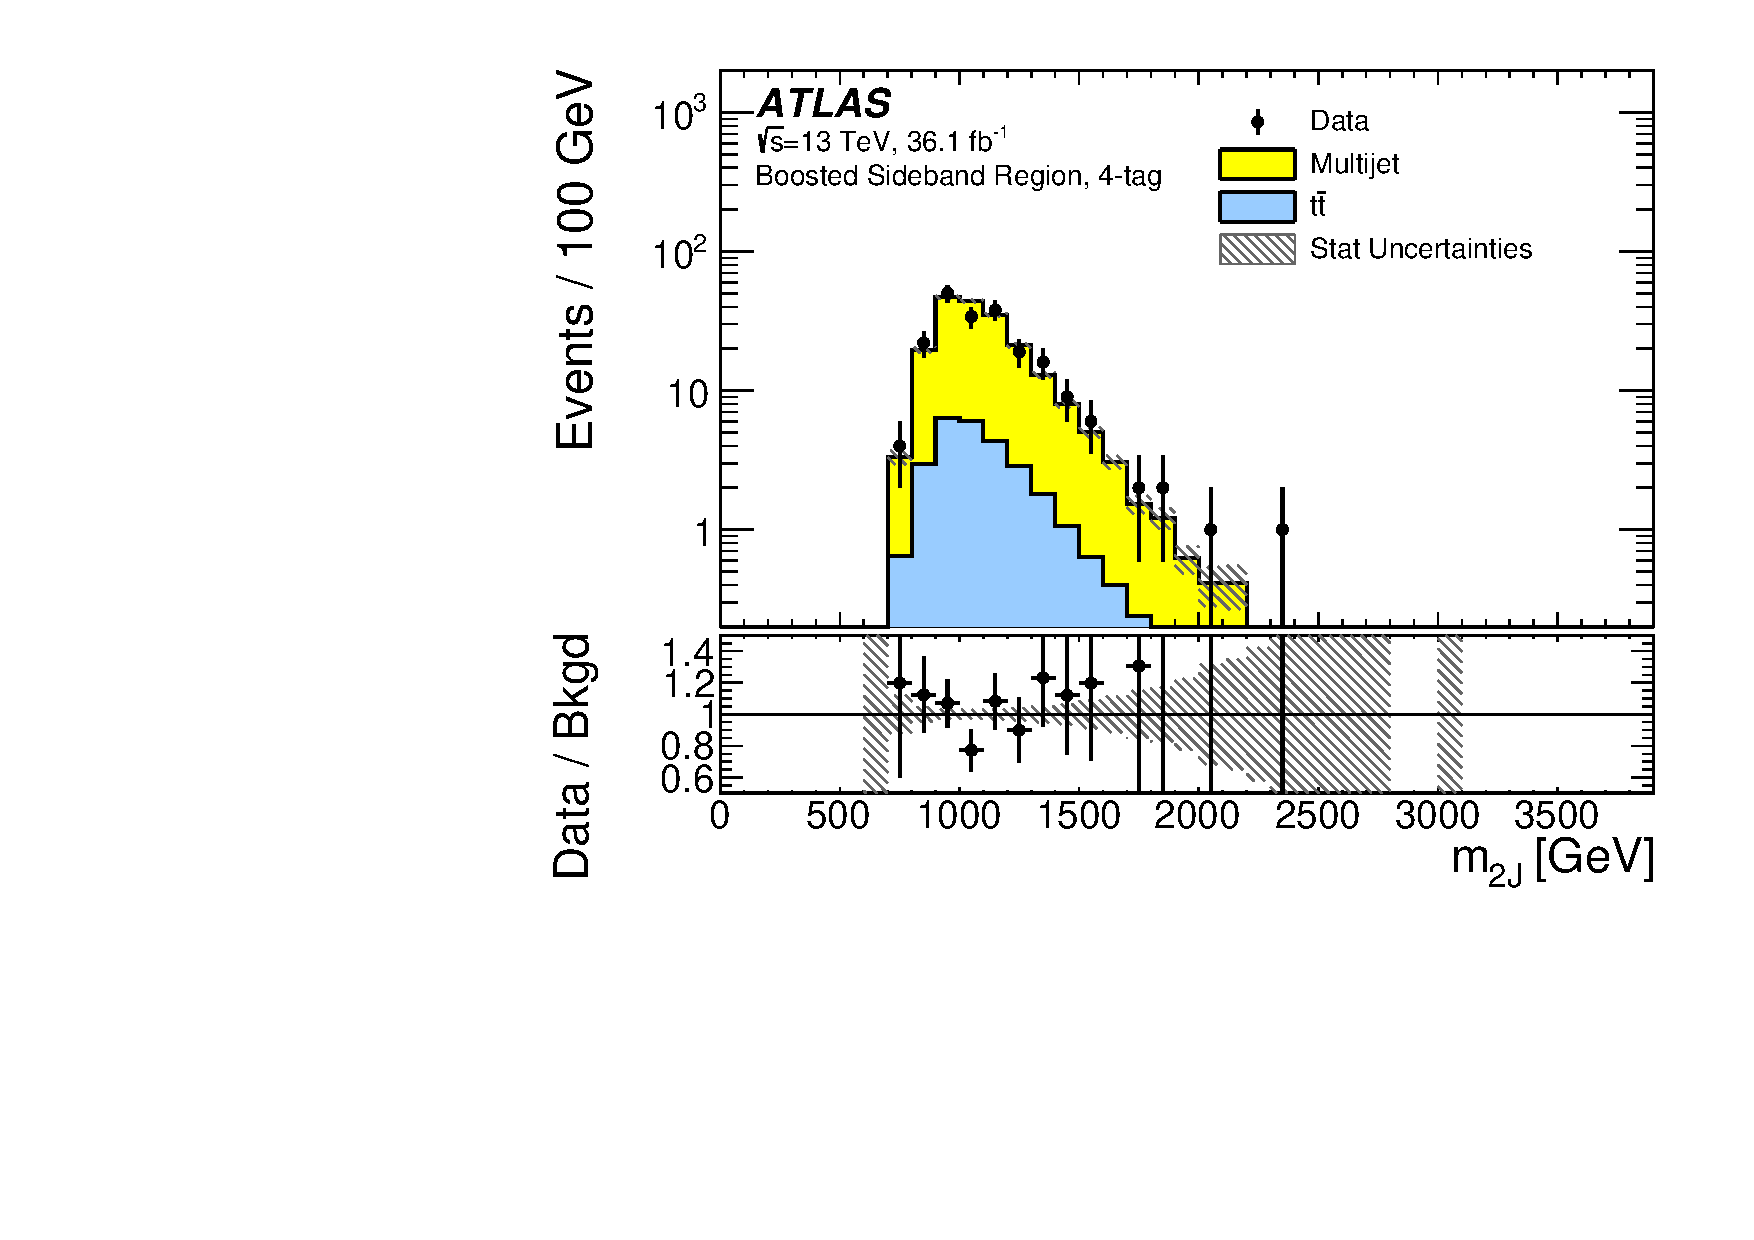
\includegraphics[width=0.35\textwidth,angle=-90]{figures/boosted/Paperplot/Moriond_bkg_9_FourTag_Sideband_mHH_l_1.pdf}
 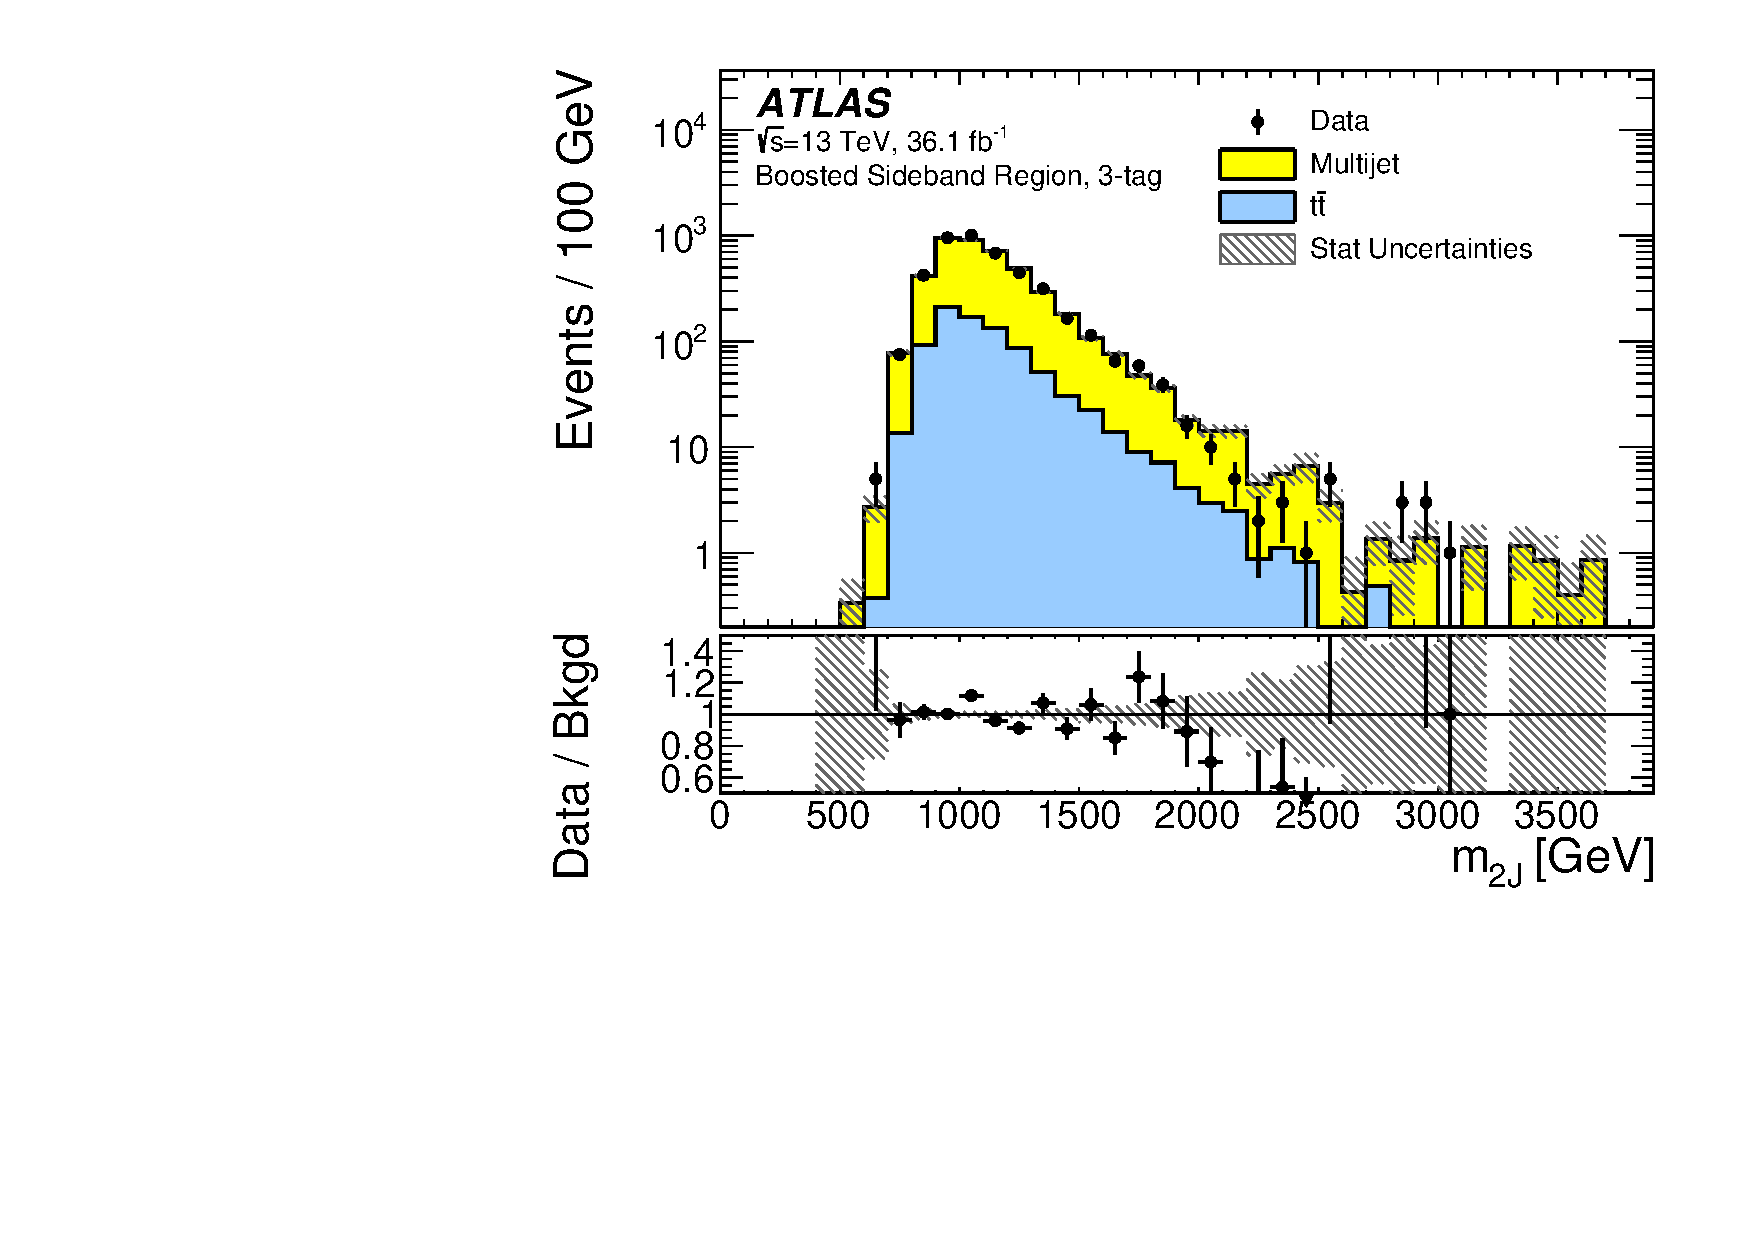
\includegraphics[width=0.35\textwidth,angle=-90]{figures/boosted/Paperplot/Moriond_bkg_9_ThreeTag_Sideband_mHH_l_1.pdf}\\
 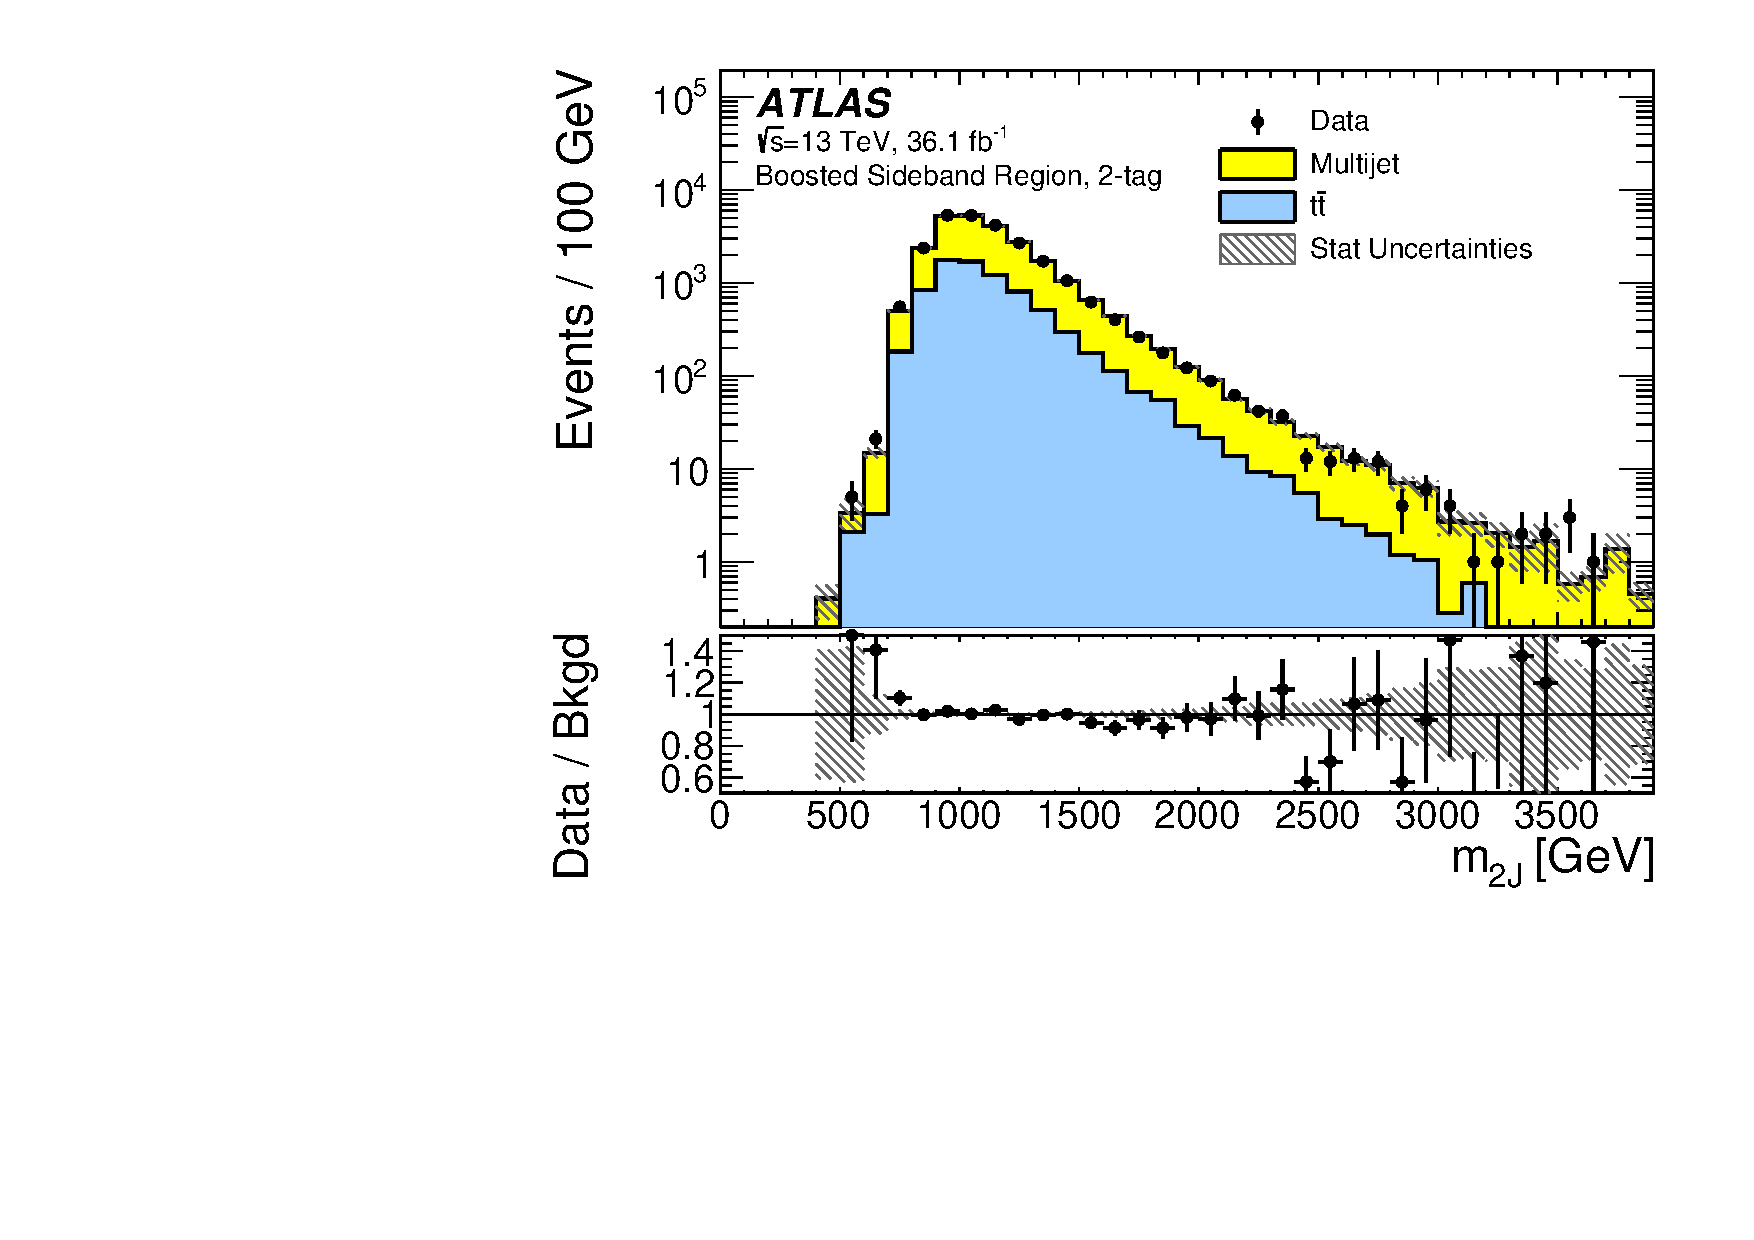
\includegraphics[width=0.35\textwidth,angle=-90]{figures/boosted/Paperplot/Moriond_bkg_9_TwoTag_split_Sideband_mHH_l_1.pdf}\\
\caption{The \mtwoJ distributions in the sideband region of the boosted analysis for the data and the predicted background for (top left) the four-tag, (top right) the three-tag, and (bottom) the two-tag split samples. The data-to-background ratio (bottom panels) shows the statistical uncertainties as the gray hatched band.}
\label{fig:boosted-sb-mjj}
\end{center}
\end{figure}

\clearpage
%%%%%%%%%%%%%%%%%%%%%%%%%%%%%%%%%%%%%%%%%%%%%%%%%%%%%%%%%%%%%%%%%%%%%%%
%%%%%%%%%%%%%%%%%%%%%%%%%%%%%%%%%%%%%%%%%%%%%%%%%%%%%%%%%%%%%%%%%%%%%%%
%%%  CR plots
%%%%%%%%%%%%%%%%%%%%%%%%%%%%%%%%%%%%%%%%%%%%%%%%%%%%%%%%%%%%%%%%%%%%%%%
%%%%%%%%%%%%%%%%%%%%%%%%%%%%%%%%%%%%%%%%%%%%%%%%%%%%%%%%%%%%%%%%%%%%%%%
\section{\mtwoJ~ in the control region}
\label{sec:boosted-cr}

\paragraph{}
Figure~\ref{fig:boosted-cr-mjj} shows comparisons of the predicted \mtwoJ~background distributions to those observed in the data in the control region.
The predicted background and observed distributions are in agreement, with no significant excess.
Other control region distributions are shown in Appendix~\ref{AppendixCR}.

\begin{figure}[htbp!]
\begin{center}
 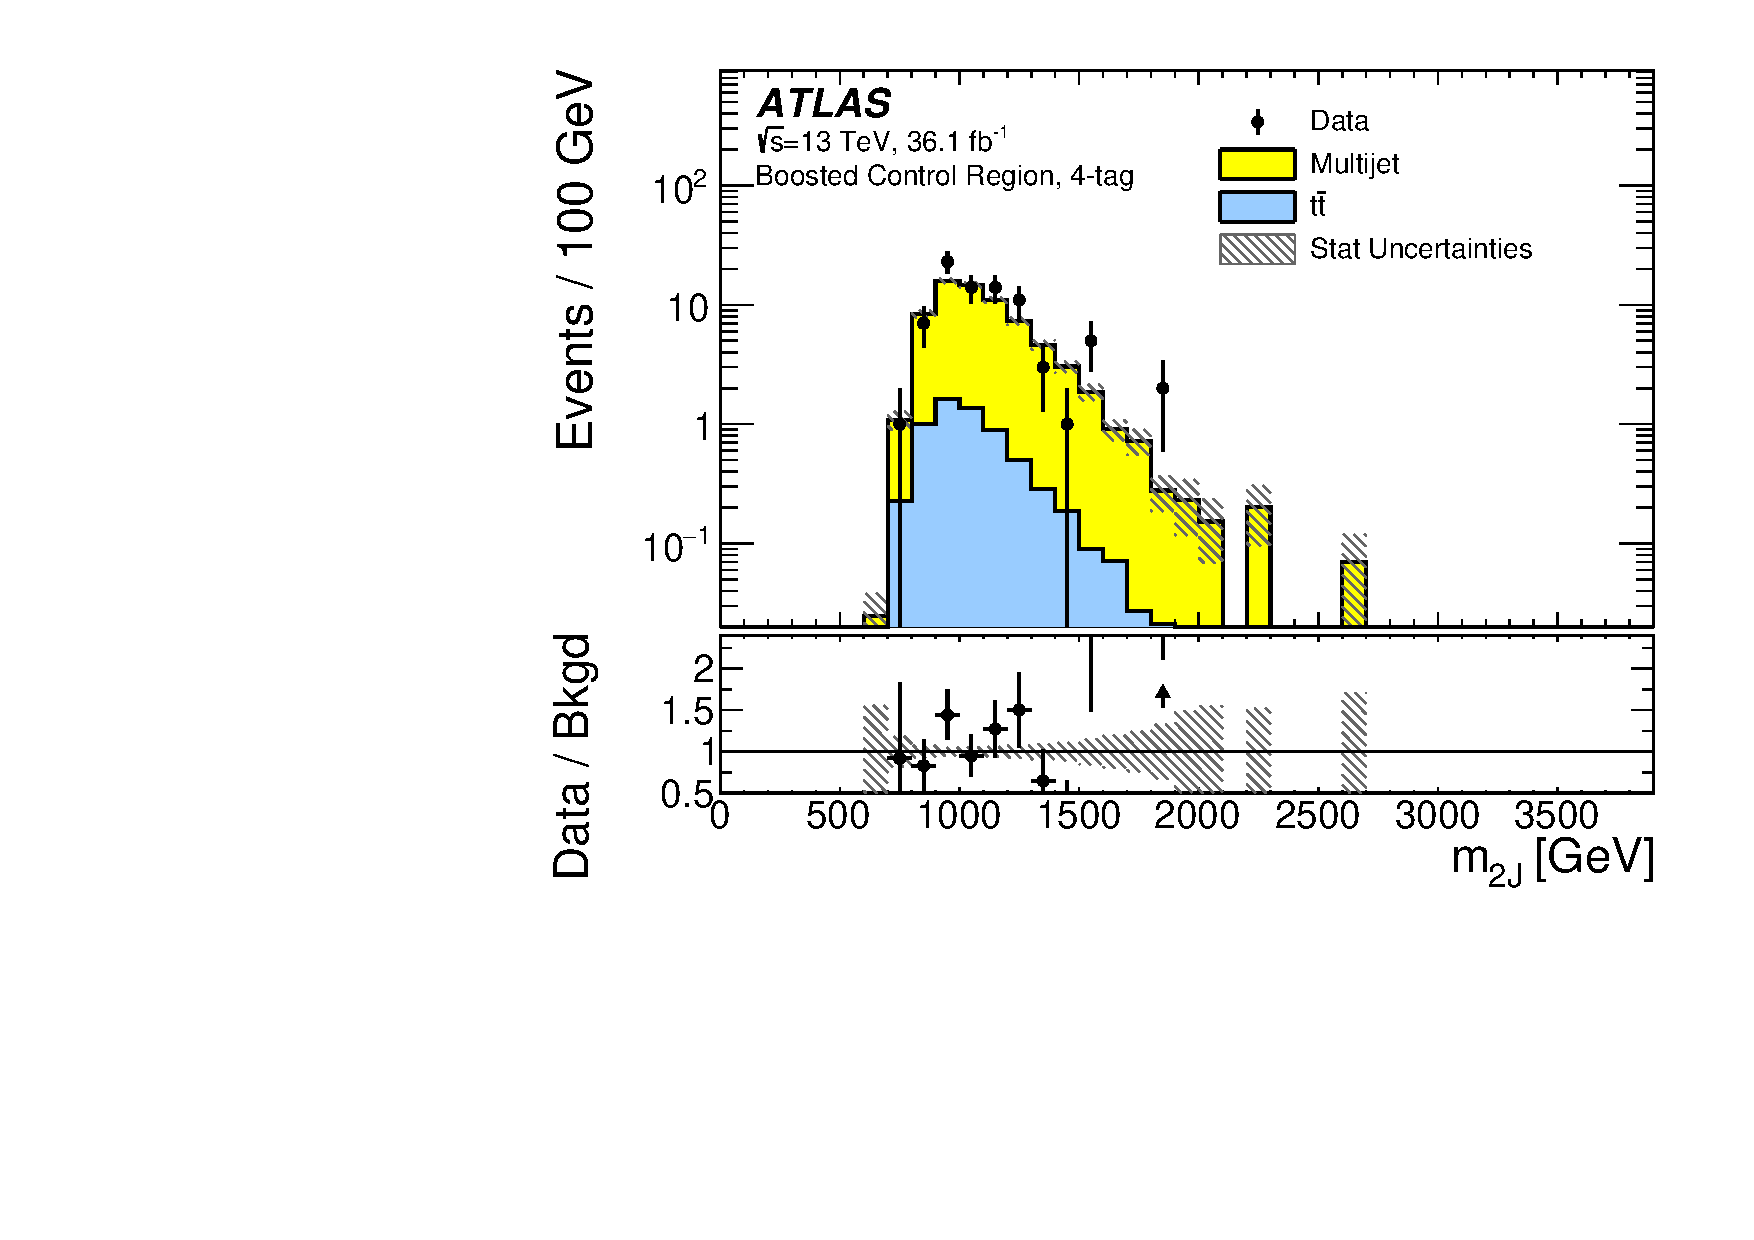
\includegraphics[width=0.35\textwidth,angle=-90]{figures/boosted/Paperplot/Moriond_bkg_9_FourTag_Control_mHH_l_1.pdf}
 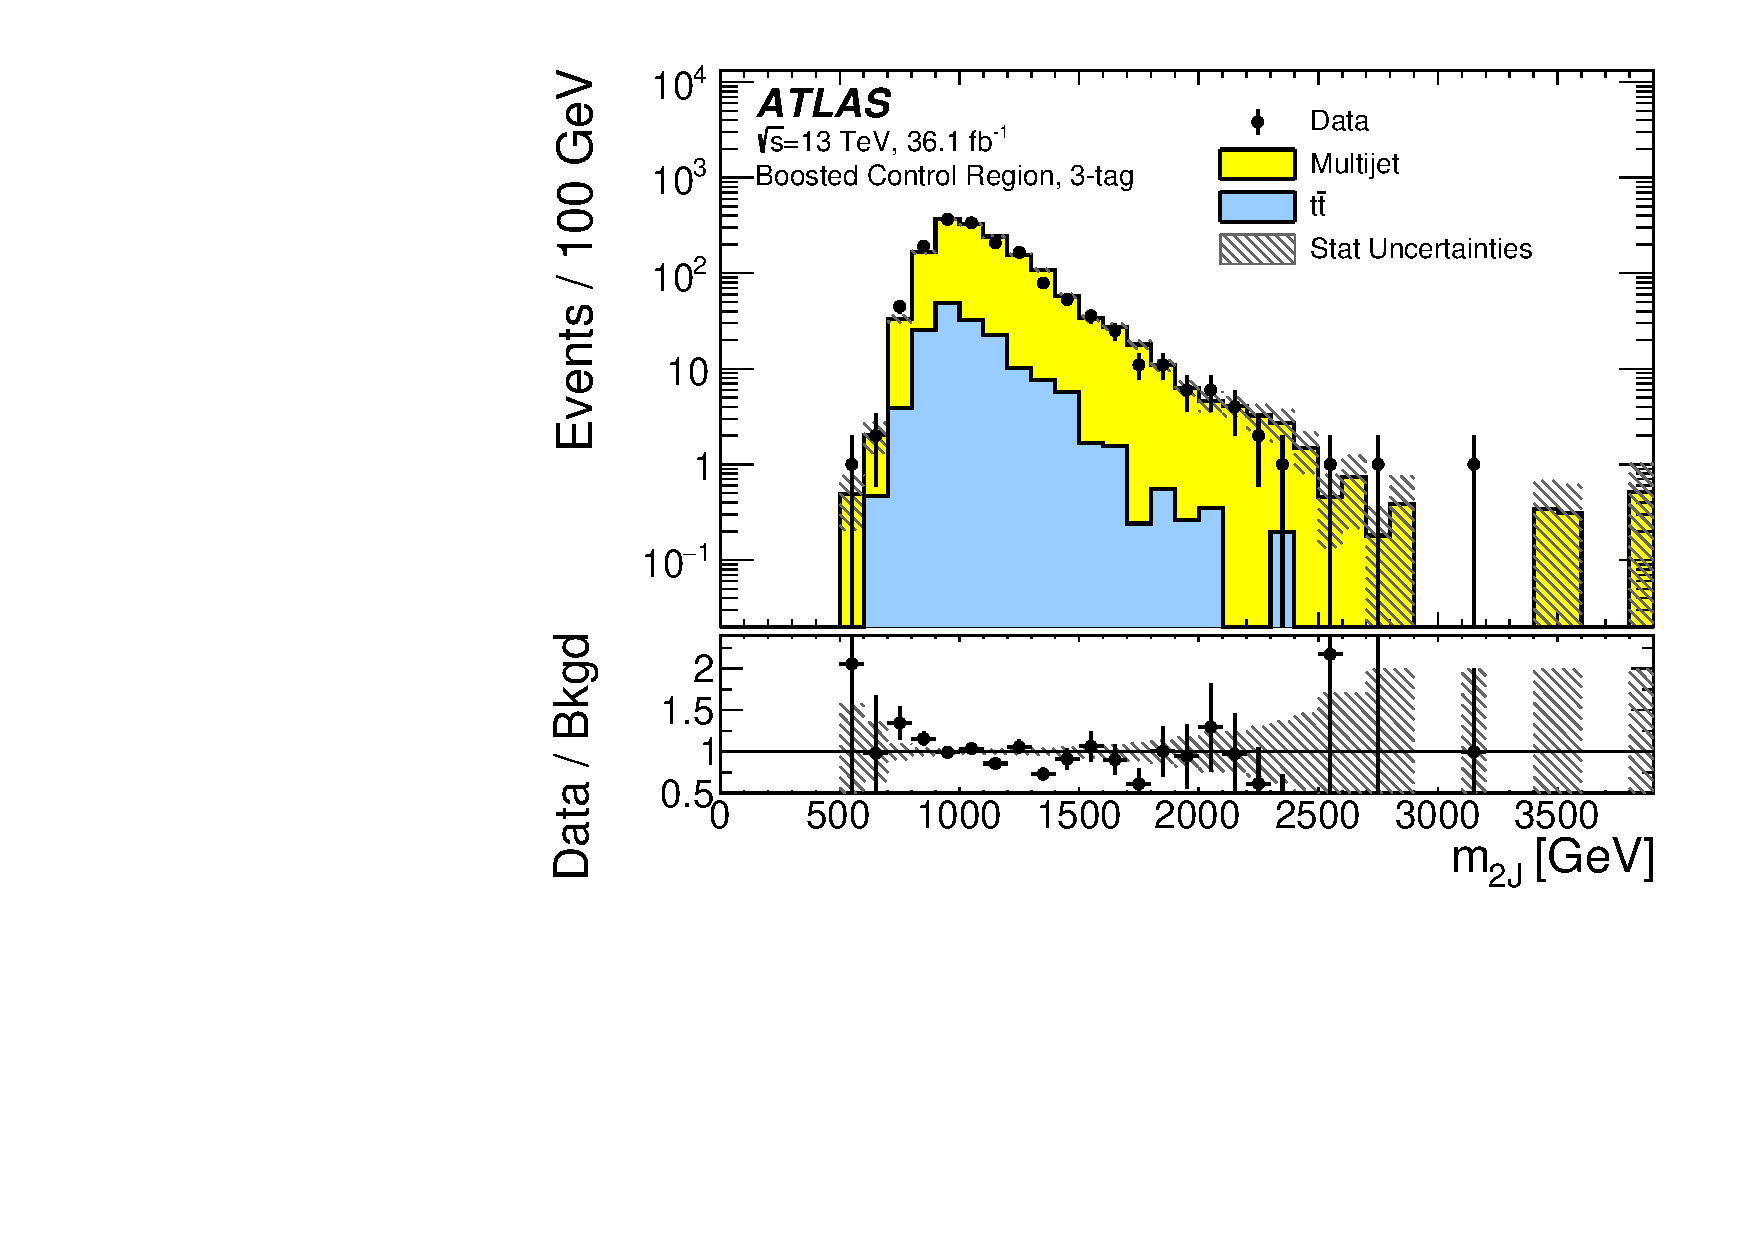
\includegraphics[width=0.35\textwidth,angle=-90]{figures/boosted/Paperplot/Moriond_bkg_9_ThreeTag_Control_mHH_l_1.pdf}\\
 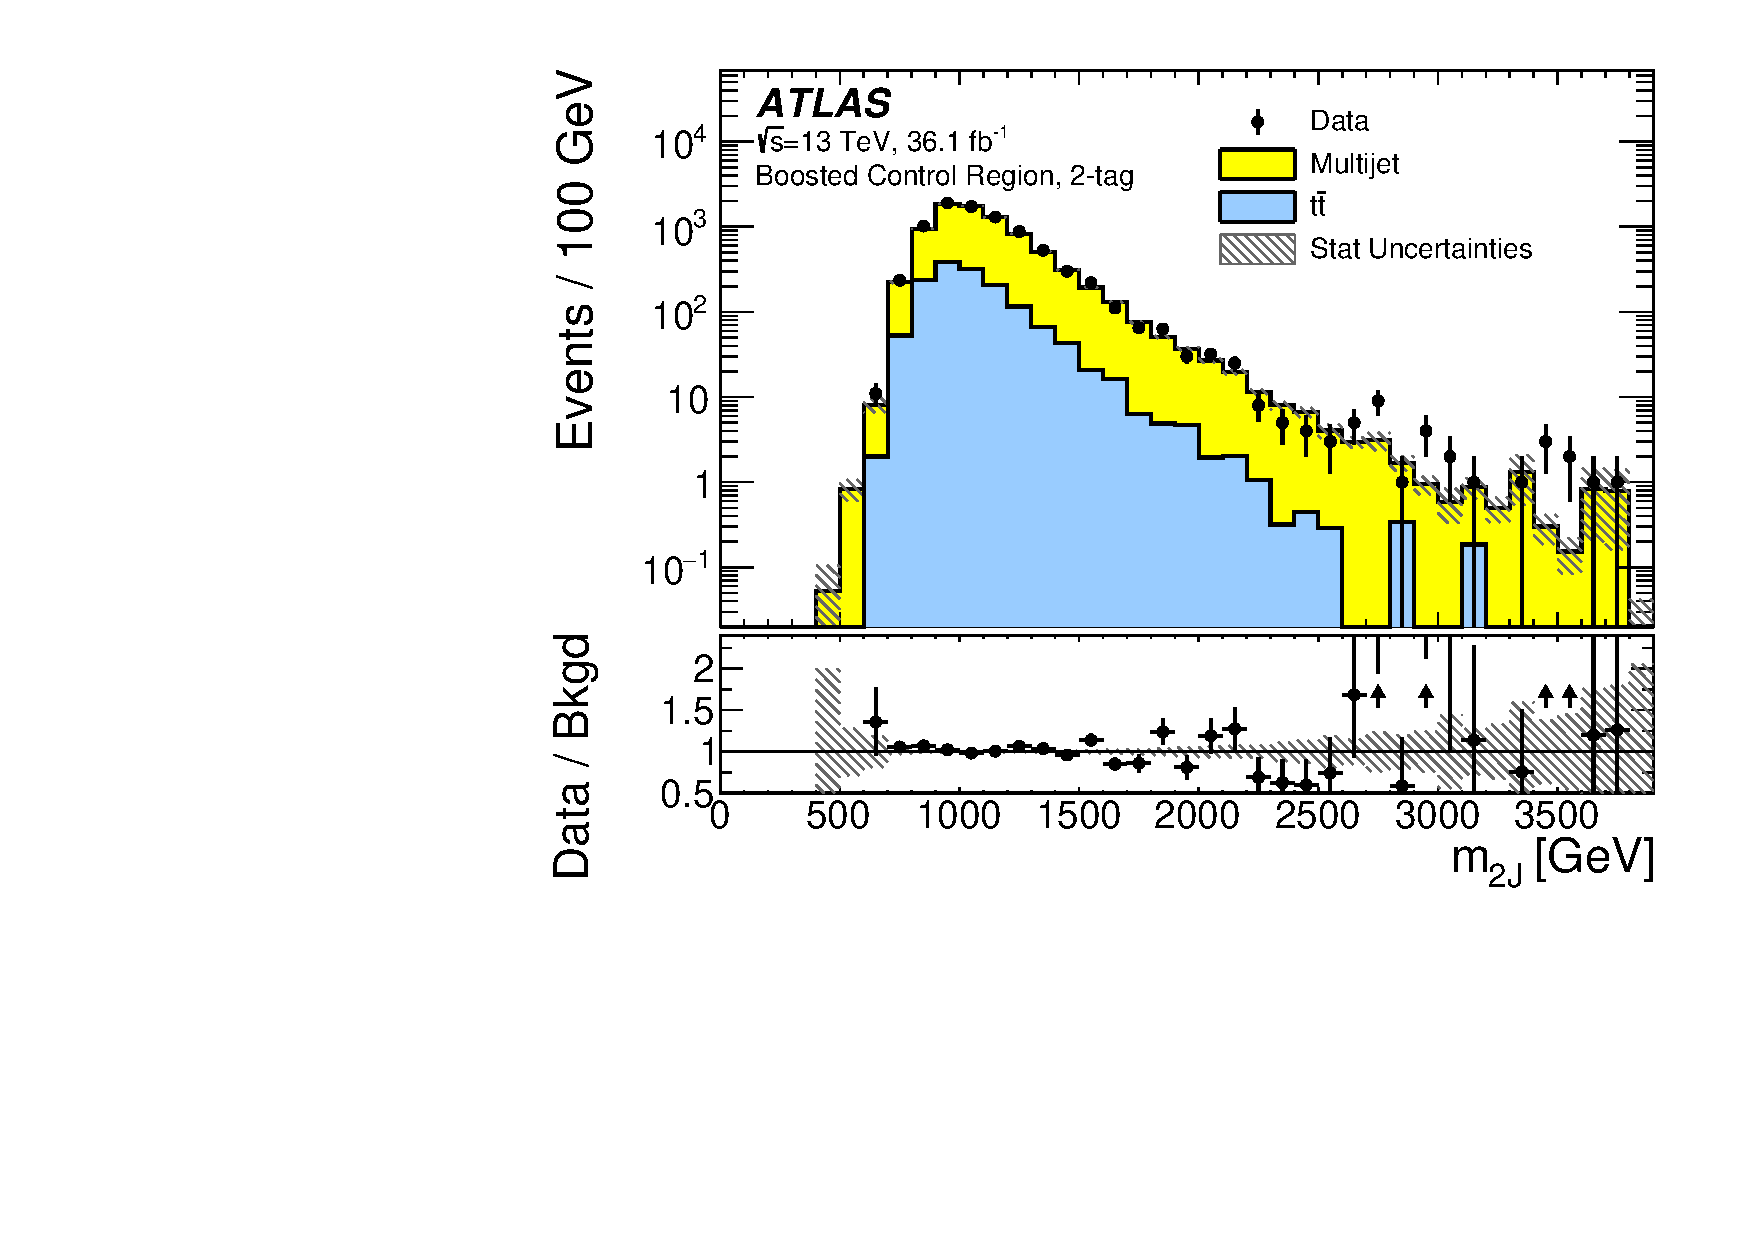
\includegraphics[width=0.35\textwidth,angle=-90]{figures/boosted/Paperplot/Moriond_bkg_9_TwoTag_split_Control_mHH_l_1.pdf}\\
\caption{The \mtwoJ distributions in the control region of the boosted analysis for the data and the predicted background for (top left) the four-tag, (top right) the three-tag, and (bottom) the two-tag split samples. The data-to-background ratio (bottom panels) shows the statistical uncertainties as the gray hatched band.}
\label{fig:boosted-cr-mjj}
\end{center}
\end{figure}


%%%%%%%%%%%%%%%%%%%%%%%%%%%%%%%%%%%%%%%%%%%%%%%%%%%%%%%%%%%%%%%%%%%%%%%
%%%%%%%%%%%%%%%%%%%%%%%%%%%%%%%%%%%%%%%%%%%%%%%%%%%%%%%%%%%%%%%%%%%%%%%
%%%  SR smoothing
%%%%%%%%%%%%%%%%%%%%%%%%%%%%%%%%%%%%%%%%%%%%%%%%%%%%%%%%%%%%%%%%%%%%%%%
%%%%%%%%%%%%%%%%%%%%%%%%%%%%%%%%%%%%%%%%%%%%%%%%%%%%%%%%%%%%%%%%%%%%%%%
\section{\mtwoJ~ rescale and smoothing in the signal region}
\label{sec:boosted-SR-smoothing}

\paragraph{}
In signal region, the four-momentum of each large-\R jet is multiplied with a factor $m_{H}/m_{\mathrm{J}}$.
From this, a scaled \mtwoJ~ is calculated.
This improves the resolution of \mtwoJ~ for signal events by correcting the energy loss.
There is little impact on the background distribution.
Using the scaled \mtwoJ~ distribution, the expected exclusion limits are slightly better at low mass and slightly worse at high mass, with differences of the order of $10\%$ than the nominal dijet mass limits.
The scaled \mtwoJ~ distribution can be found in Figure~\ref{fig:signal-region-bkg-scaled}.

\begin{figure}[htbp!]
\begin{center}
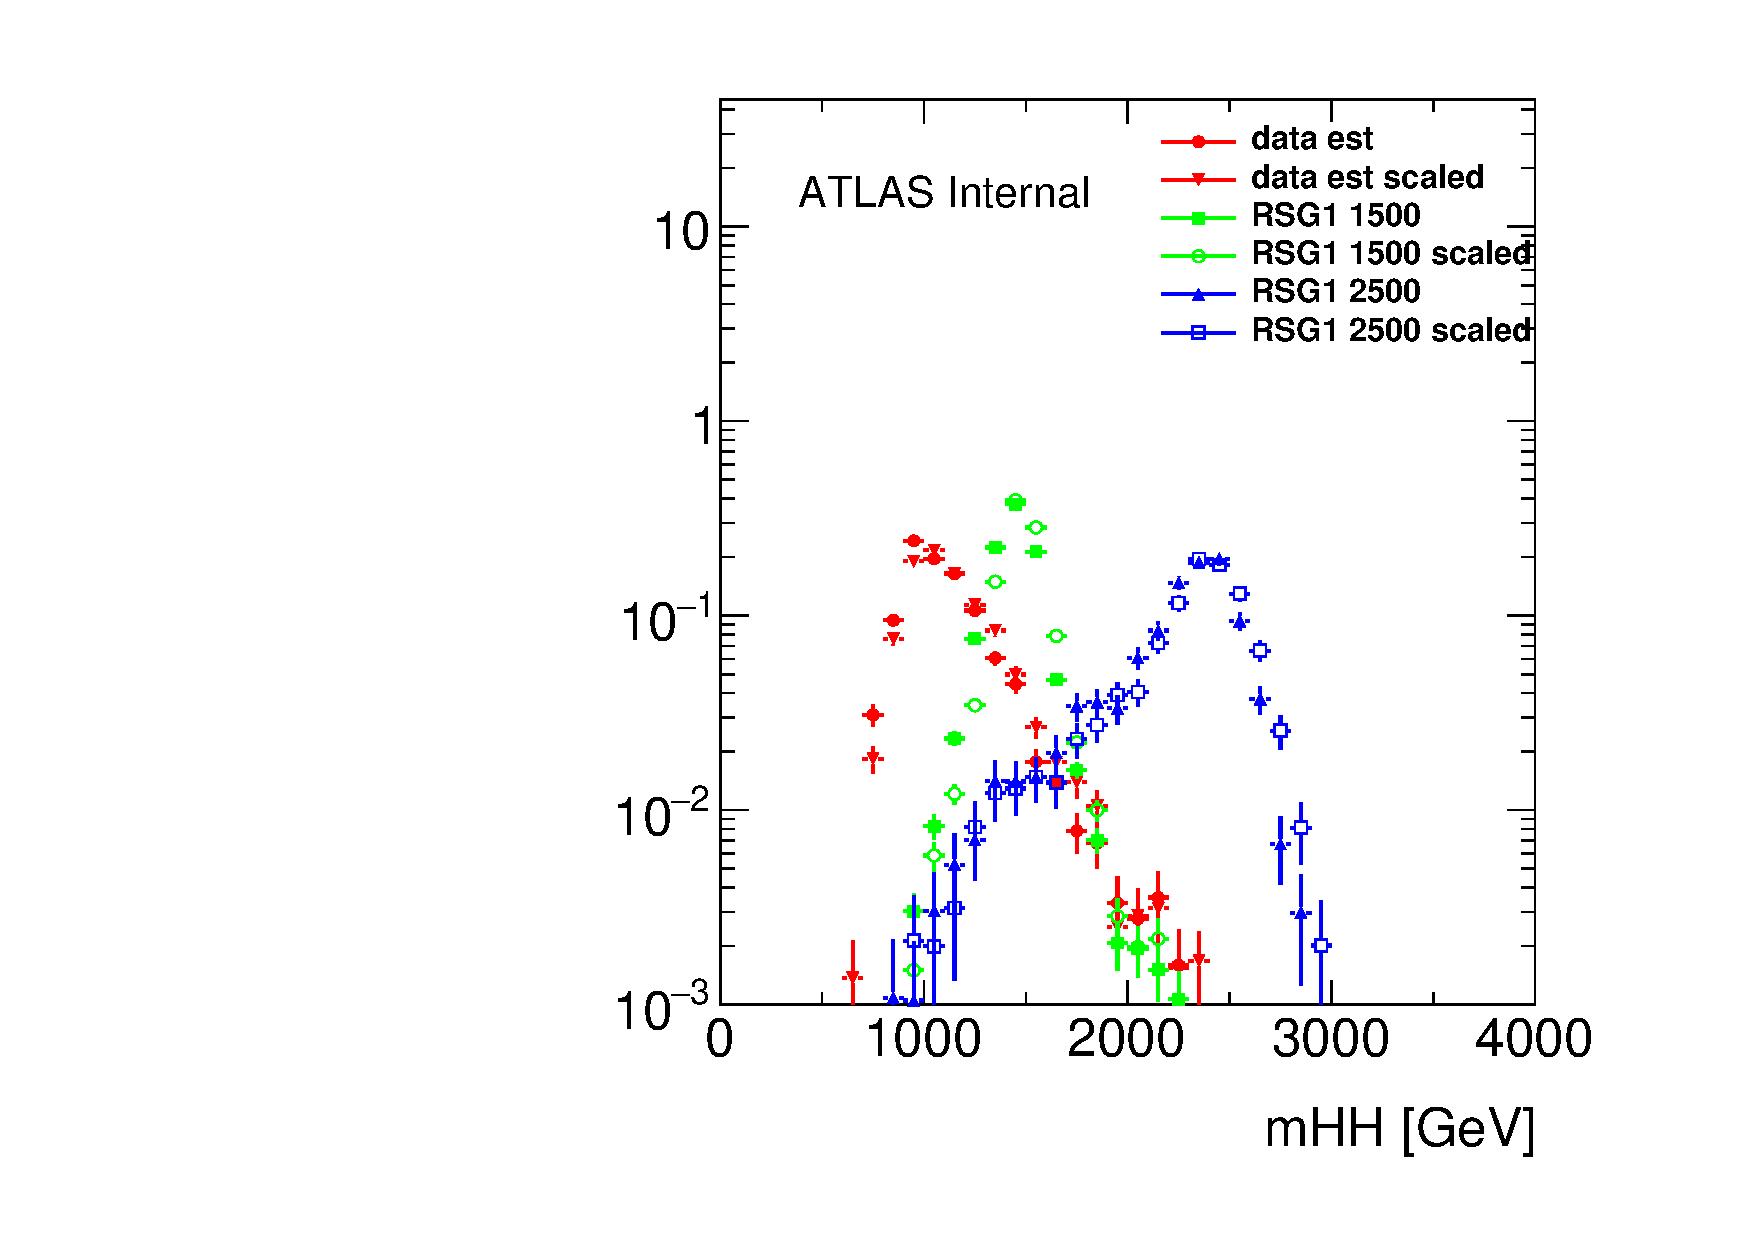
\includegraphics[width=0.3\textwidth,angle=-90]{figures/boosted/Other/FourTag_Signal_compare_scale_mHH_1.pdf}
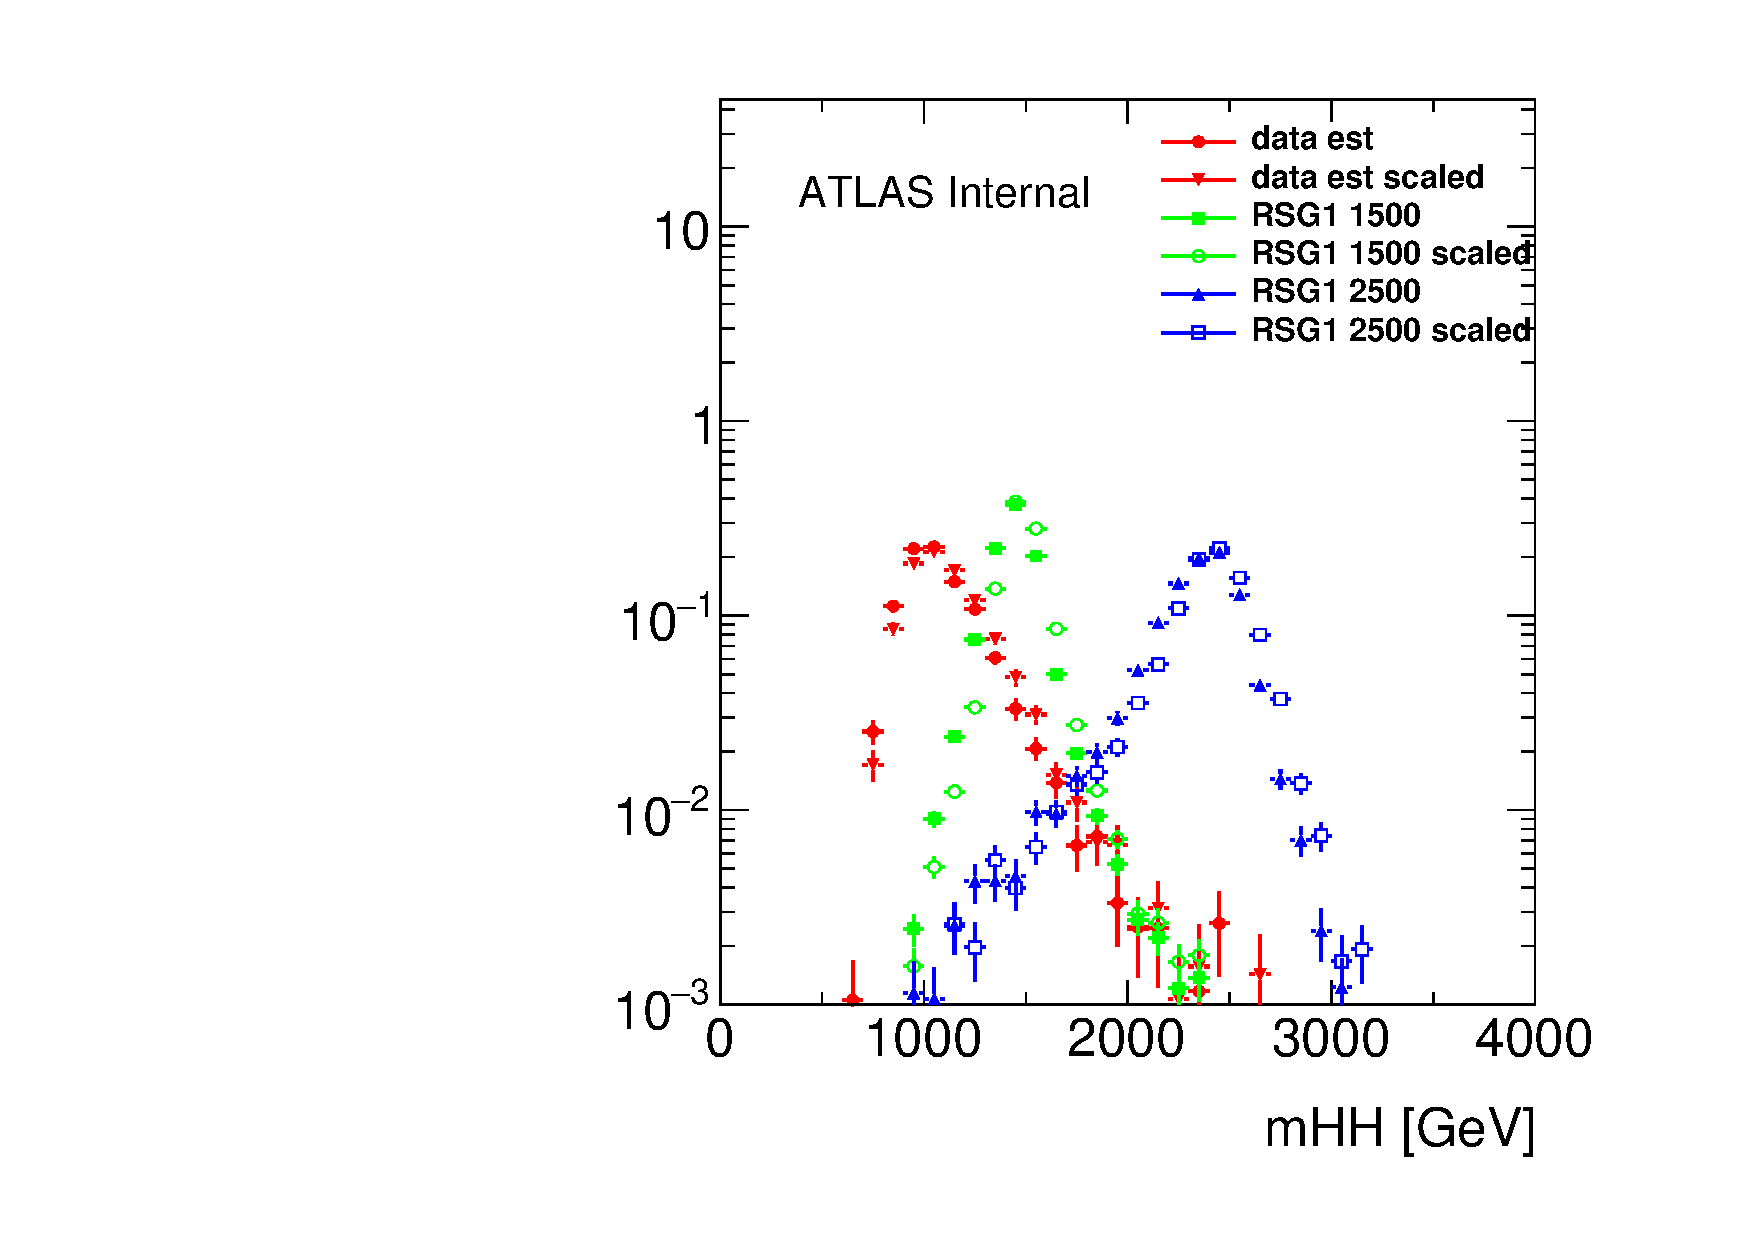
\includegraphics[width=0.3\textwidth,angle=-90]{figures/boosted/Other/ThreeTag_Signal_compare_scale_mHH_1.pdf}
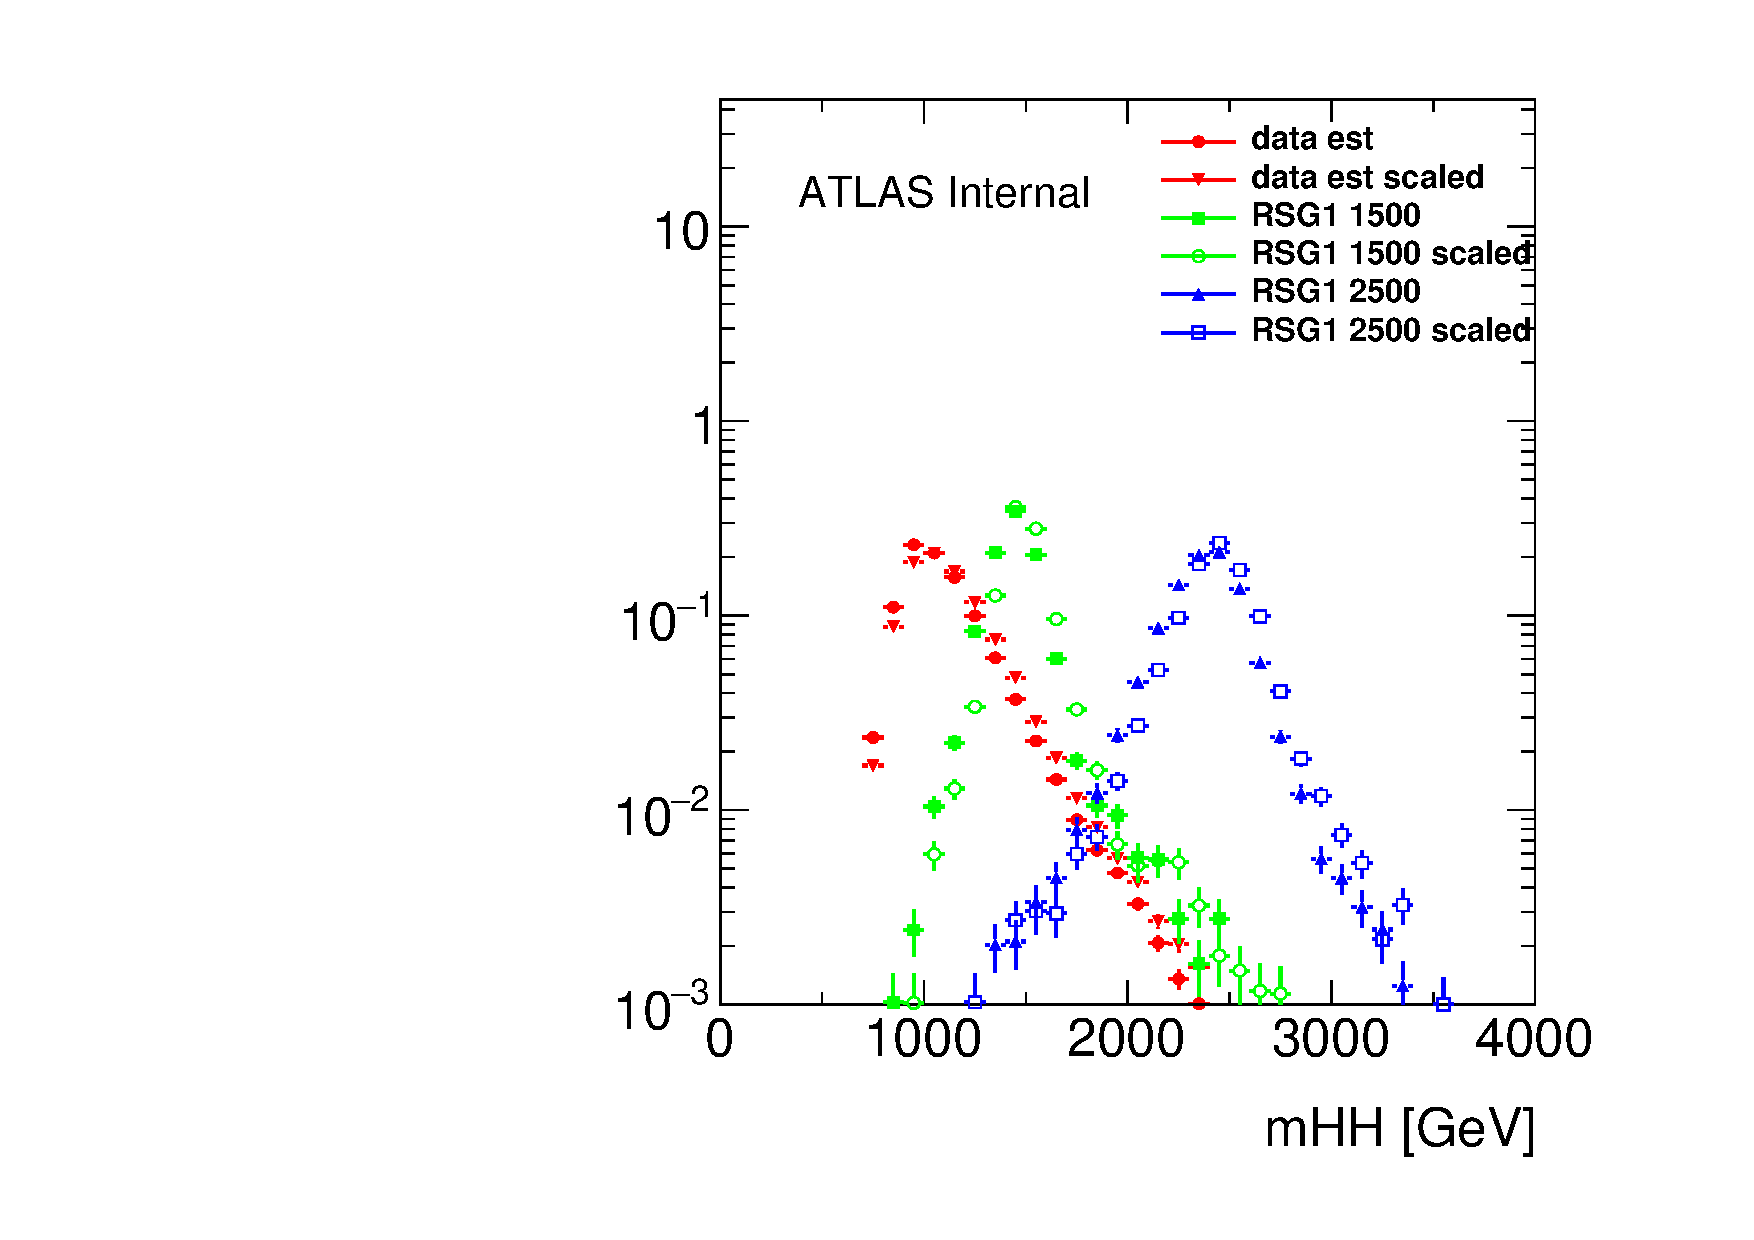
\includegraphics[width=0.3\textwidth,angle=-90]{figures/boosted/Other/TwoTag_split_Signal_compare_scale_mHH_1.pdf}
\caption{Normalized scaled \mtwoJ~ distributions for the $4b$ (left), $3b$ (middle), and $2bs$ (right) signal regions. For comparison, the unscaled  \mtwoJ~ distributions are shown on the same plot. }
\label{fig:signal-region-bkg-scaled}
\end{center}
\end{figure}

\paragraph{} 
Due to the limited $1/2b$ statistics at high \mtwoJ~ above $2500$ \GeV~ and the limited \ttbar\ statistics above $1100$ \GeV~, different fits are performed to smooth the \mtwoJ~ mass distribution in the signal region. 
The $4/3/2bs$ QCD and \ttbar~ signal region scaled \mtwoJ~ distributions are fitted with the following functional form:
\begin{equation}
\label{eq:boosted_dijet}
y = \frac{a}{\frac{x}{\sqrt{s}}^2} (1-\frac{x}{\sqrt{s}})^{b - c\ \log(\frac{x}{\sqrt{s}})}
\end{equation}
where $\sqrt{s} = 13000$ \GeV~, the fit range is for $1200 < M_{JJ} < 3000$ \GeV~, and the three free parameters are a, b and c.
The values of the estimated fit parameters in the $4b$ and $3b$ and $2bs$ signal regions can be found in Table~\ref{tab:smoothparams_pole}.
Figure~\ref{fig:signal-region-mjjscaled-smoothing} shows the smoothing fits for the QCD background and the \ttbar\ background in the $4b$, $3b$, and $2bs$ signal regions.
The smoothing fit statistical uncertainties are also shown on these two plots. 
Given that the similar $1/2b$ sample is used for deriving the QCD shape for the $4/3/2bs$  signal regions, the slope parameters ($a$) are similar for  $4/3/2bs$ QCD backgrounds.

\paragraph{}
The final signal region prediction, using scaled di-jet mass distribution, with only statistical uncertainties, are shown in Figure~\ref{fig:signal-region-mjjscaled-smooth-bkg-noSYS}. 
This includes smoothing statistical uncertainties only. 
Uncertainties on the fit parameters are propagated as systematic uncertainties, though they are essentially replacing the bin-by-bin statistical uncertainties of the background estimates (which are not used once smoothing is applied).
More details on other systematics, including smoothing systematics, shape uncertainties and other sources of uncertainties would be discussed in Section~\ref{unc-smooth-qcd-in-sr}.

\begin{table}[htbp!]
\begin{center}
\caption{Smoothing parameters in $4b$ and $3b$ and $2bs$ signal regions for scaled mass distributions, the correlation between parameters is almost always 0.99.}
\begin{footnotesize} 
\begin{tabular}{c|c|c|c|c|c|c} 
Region & $ a_{t\bar{t}}$ & $ b_{t\bar{t}}$ & $ c_{t\bar{t}}$ & $ a_{qcd}$ & $ b_{qcd}$ & $c_{qcd}$ \\ 
\hline\hline 
& & & & & &\\ 
FourTag & -2.02 $\pm$ 1.17 & 42.46 $\pm$ 9.87 & 1.31 $\pm$ 8.98 & -0.49 $\pm$ 1.59 & 53.06 $\pm$ 15.2 & -11.1 $\pm$ 12.8\\ 
ThreeTag & 1.84 $\pm$ 1.17 & 42.45 $\pm$ 9.88 & 1.32 $\pm$ 8.98 & 8.51 $\pm$ 0.98 & -13.8 $\pm$ 9.14 & 42.58 $\pm$ 7.87\\ 
TwoTag split & 4.22 $\pm$ 1.17 & 42.45 $\pm$ 9.88 & 1.32 $\pm$ 8.98 & 7.06 $\pm$ 0.32 & 11.54 $\pm$ 2.77 & 19.05 $\pm$ 2.48\\ 
& & & & & &\\ 
\hline\hline 
\end{tabular} 
\end{footnotesize} 
\newline 

\label{tab:smoothparams_pole}
\end{center}
\end{table}

\begin{figure}[htbp!]
\begin{center}
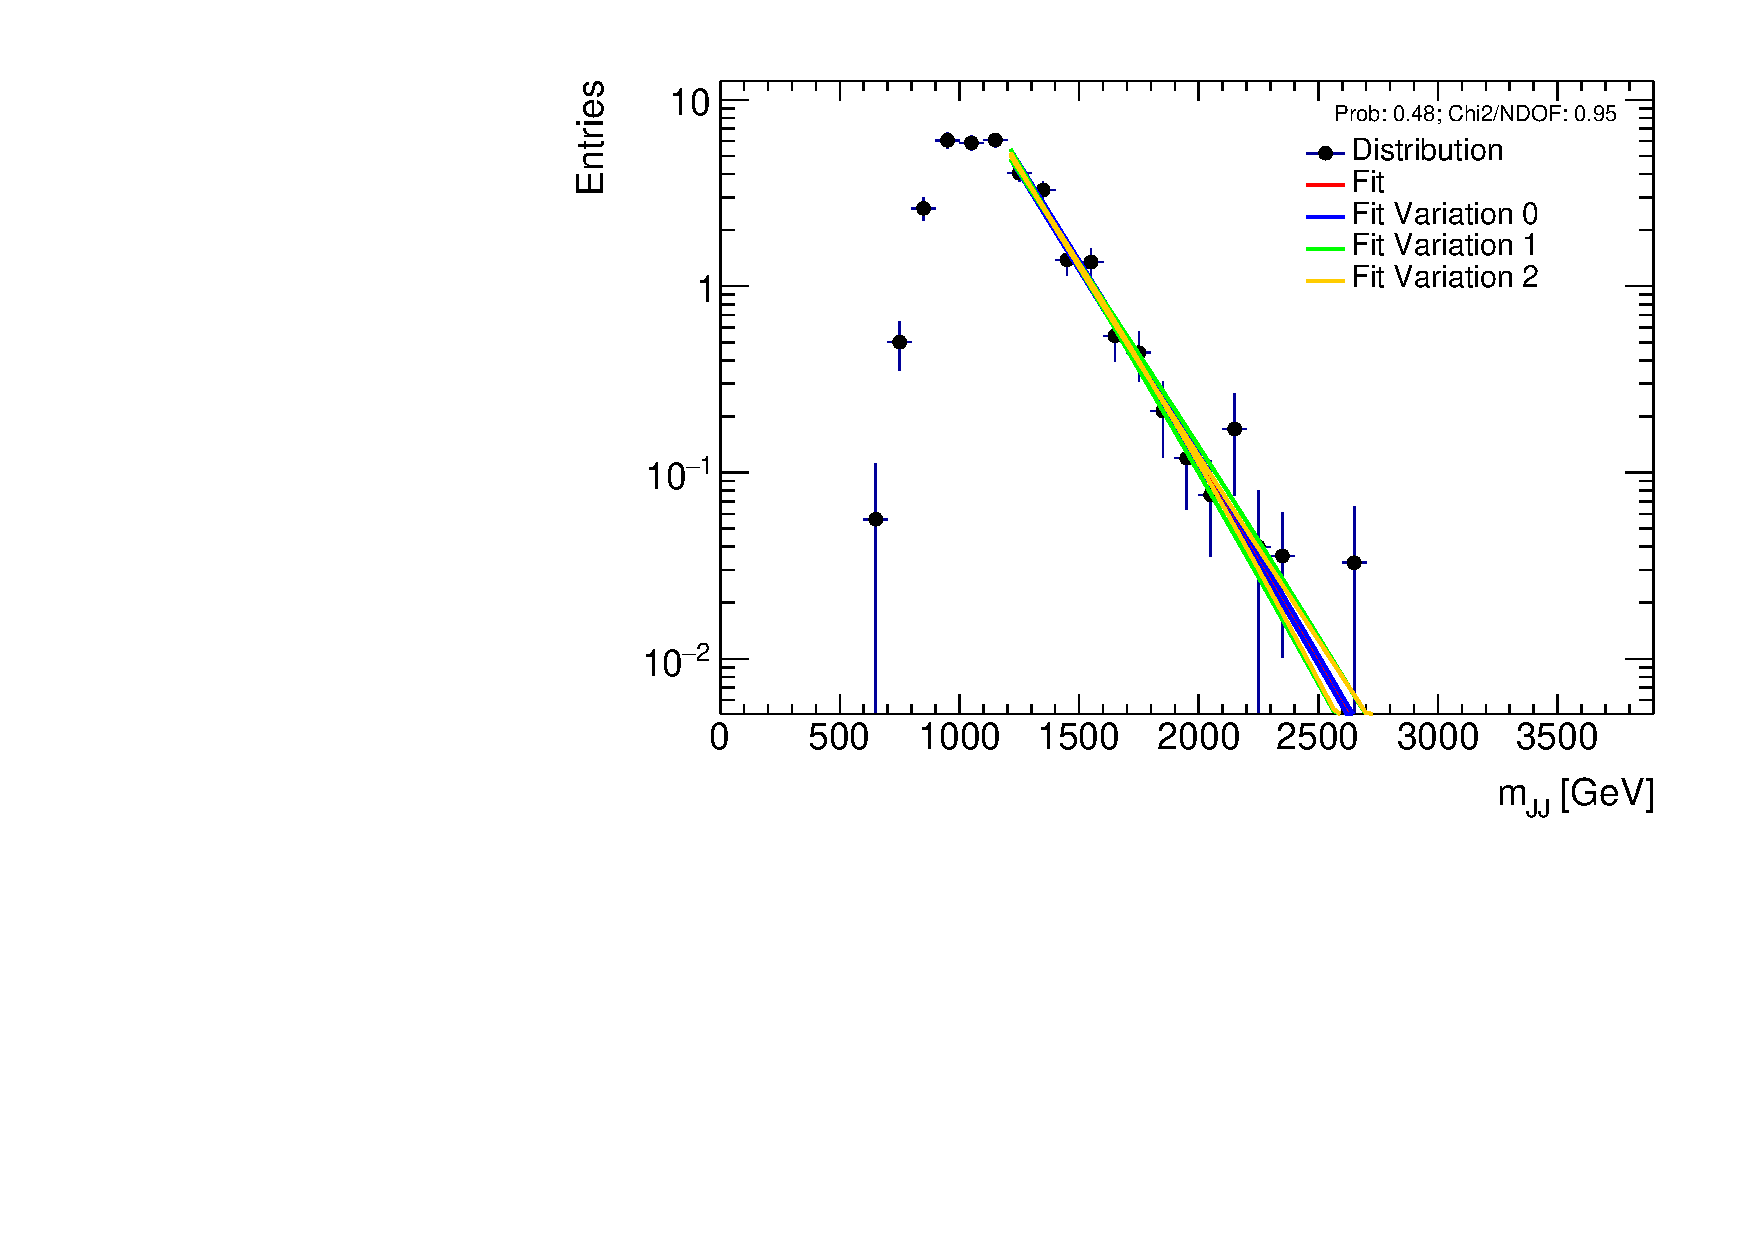
\includegraphics[width=0.3\textwidth,angle=-90]{figures/boosted/Smooth/qcd_est_FourTag_Signal_mHH_pole_l.pdf}
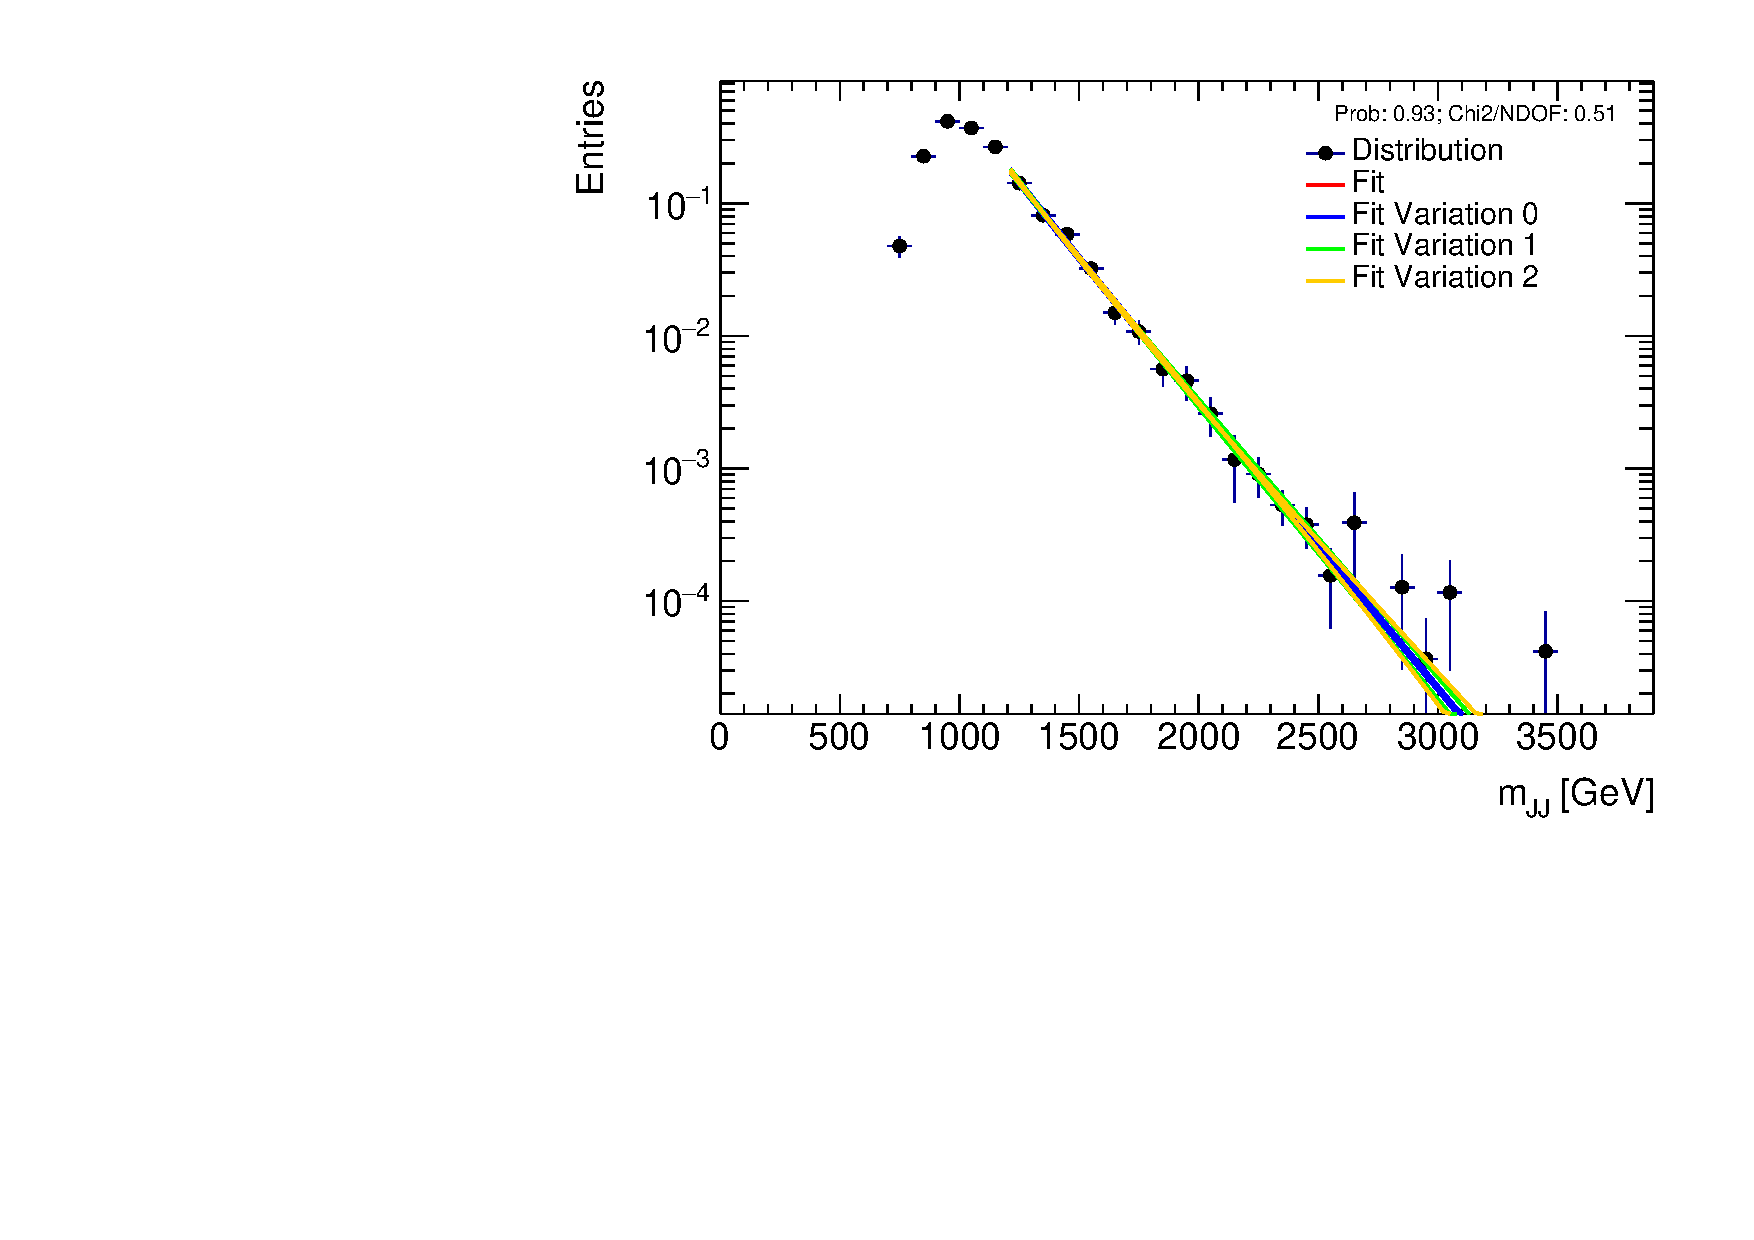
\includegraphics[width=0.3\textwidth,angle=-90]{figures/boosted/Smooth/ttbar_est_FourTag_Signal_mHH_pole_l.pdf} \\ 
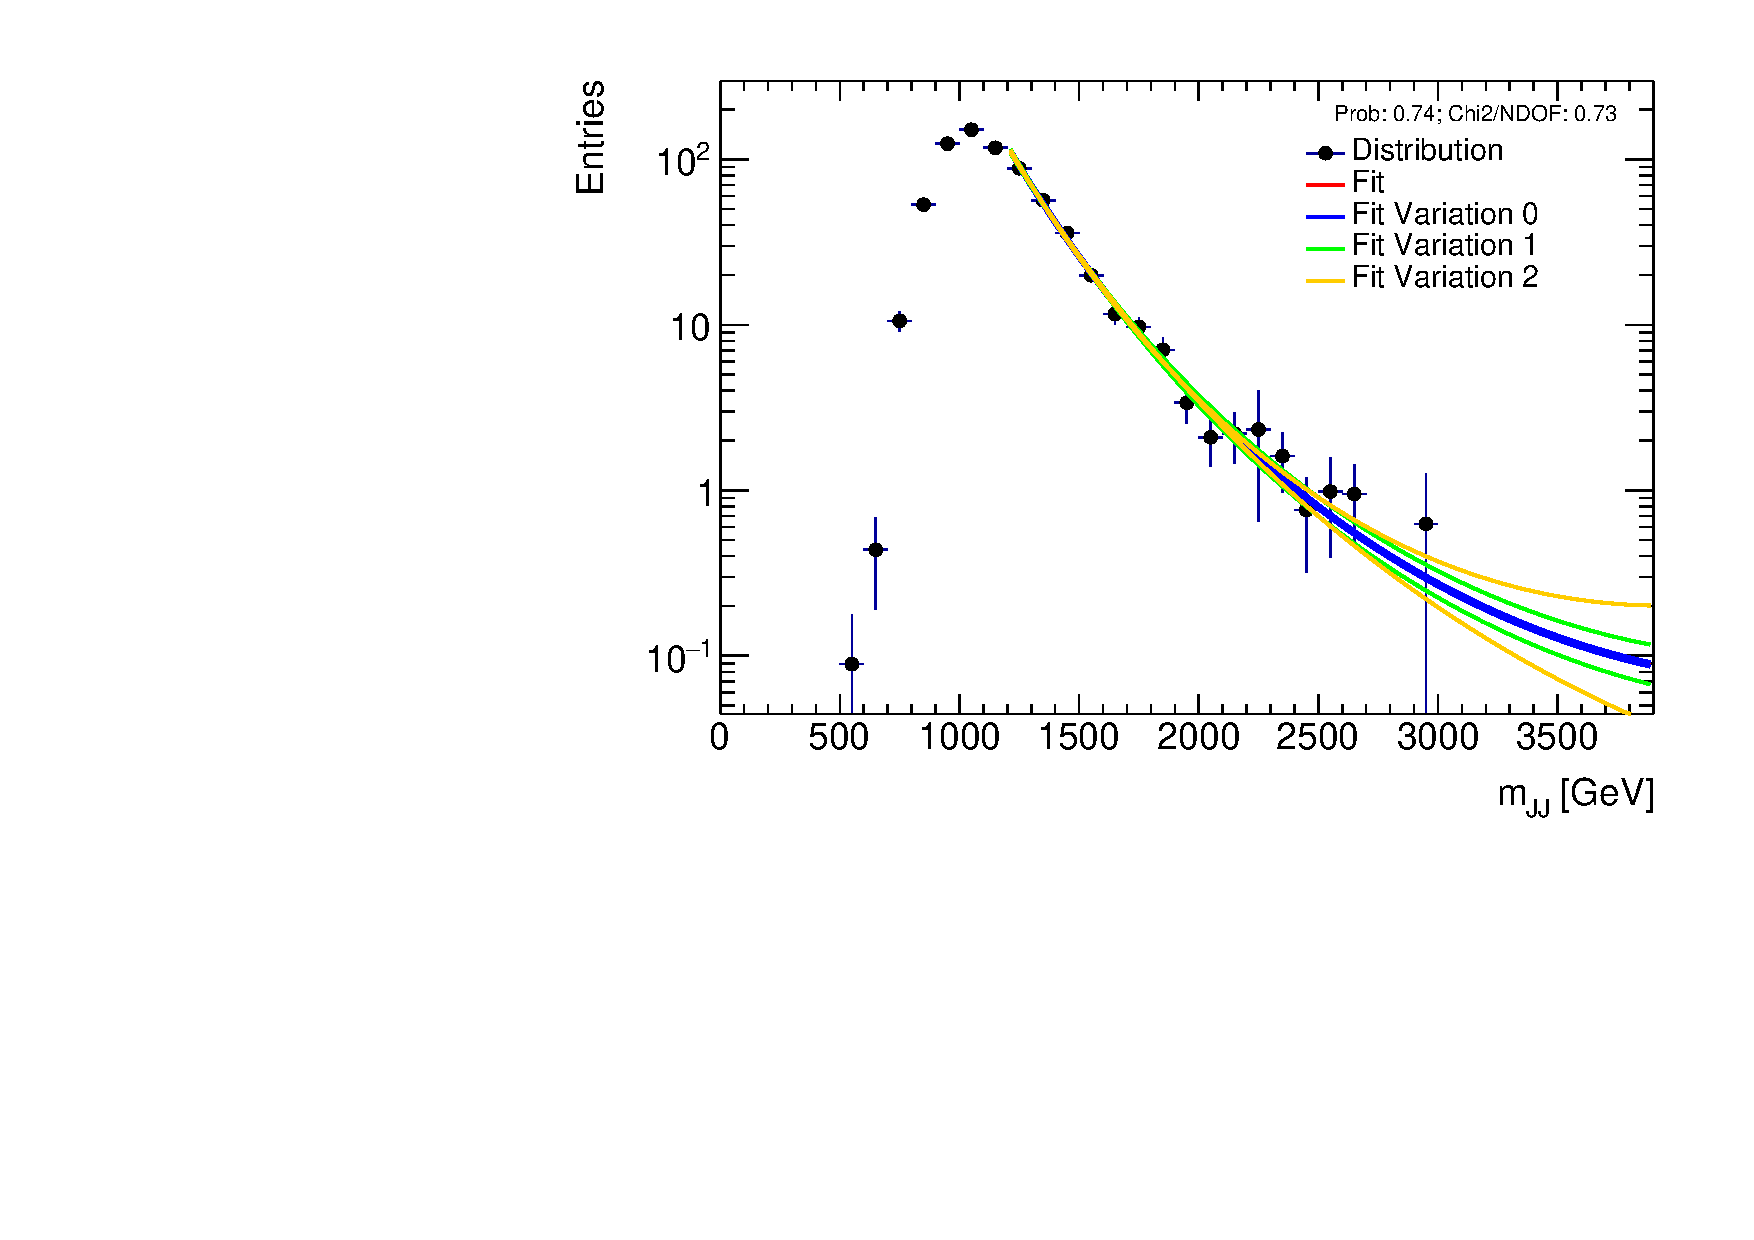
\includegraphics[width=0.3\textwidth,angle=-90]{figures/boosted/Smooth/qcd_est_ThreeTag_Signal_mHH_pole_l.pdf}
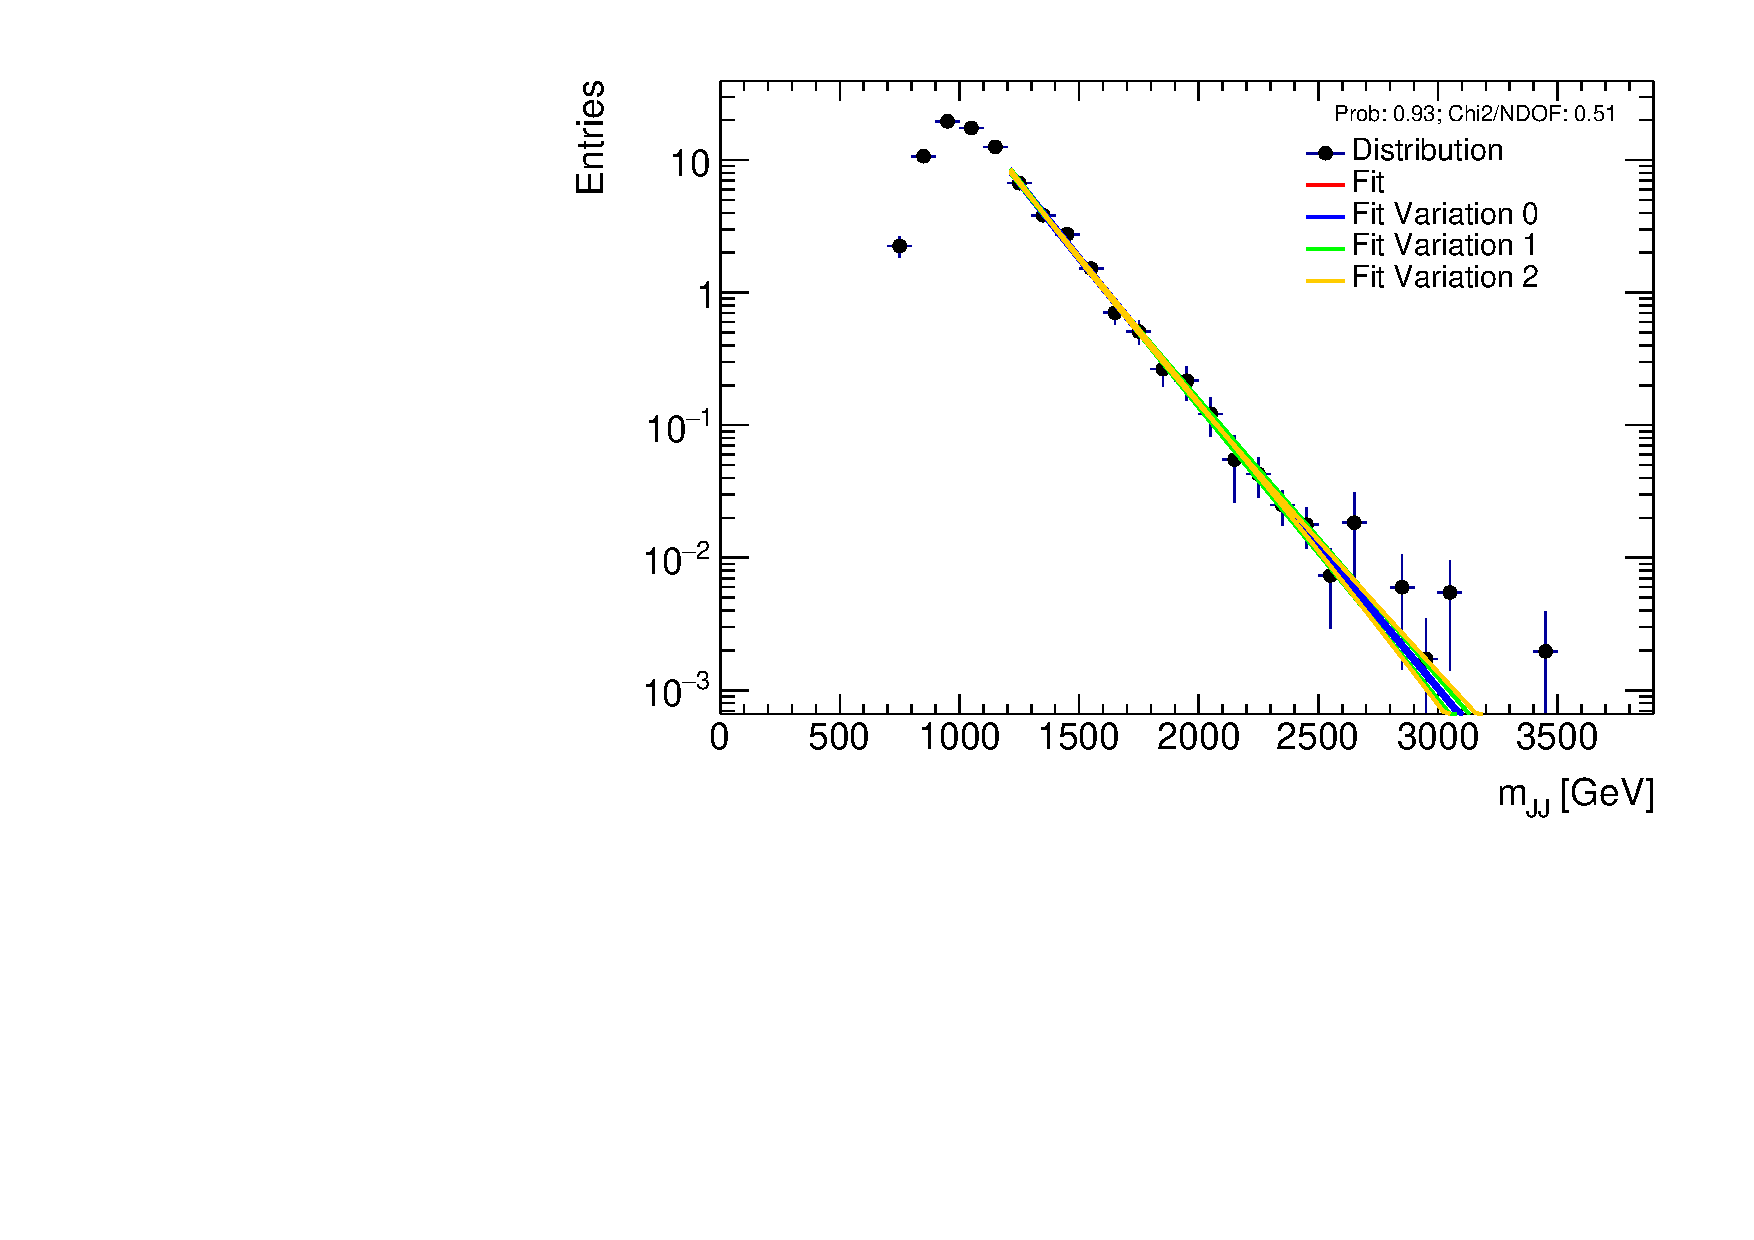
\includegraphics[width=0.3\textwidth,angle=-90]{figures/boosted/Smooth/ttbar_est_ThreeTag_Signal_mHH_pole_l.pdf}\\
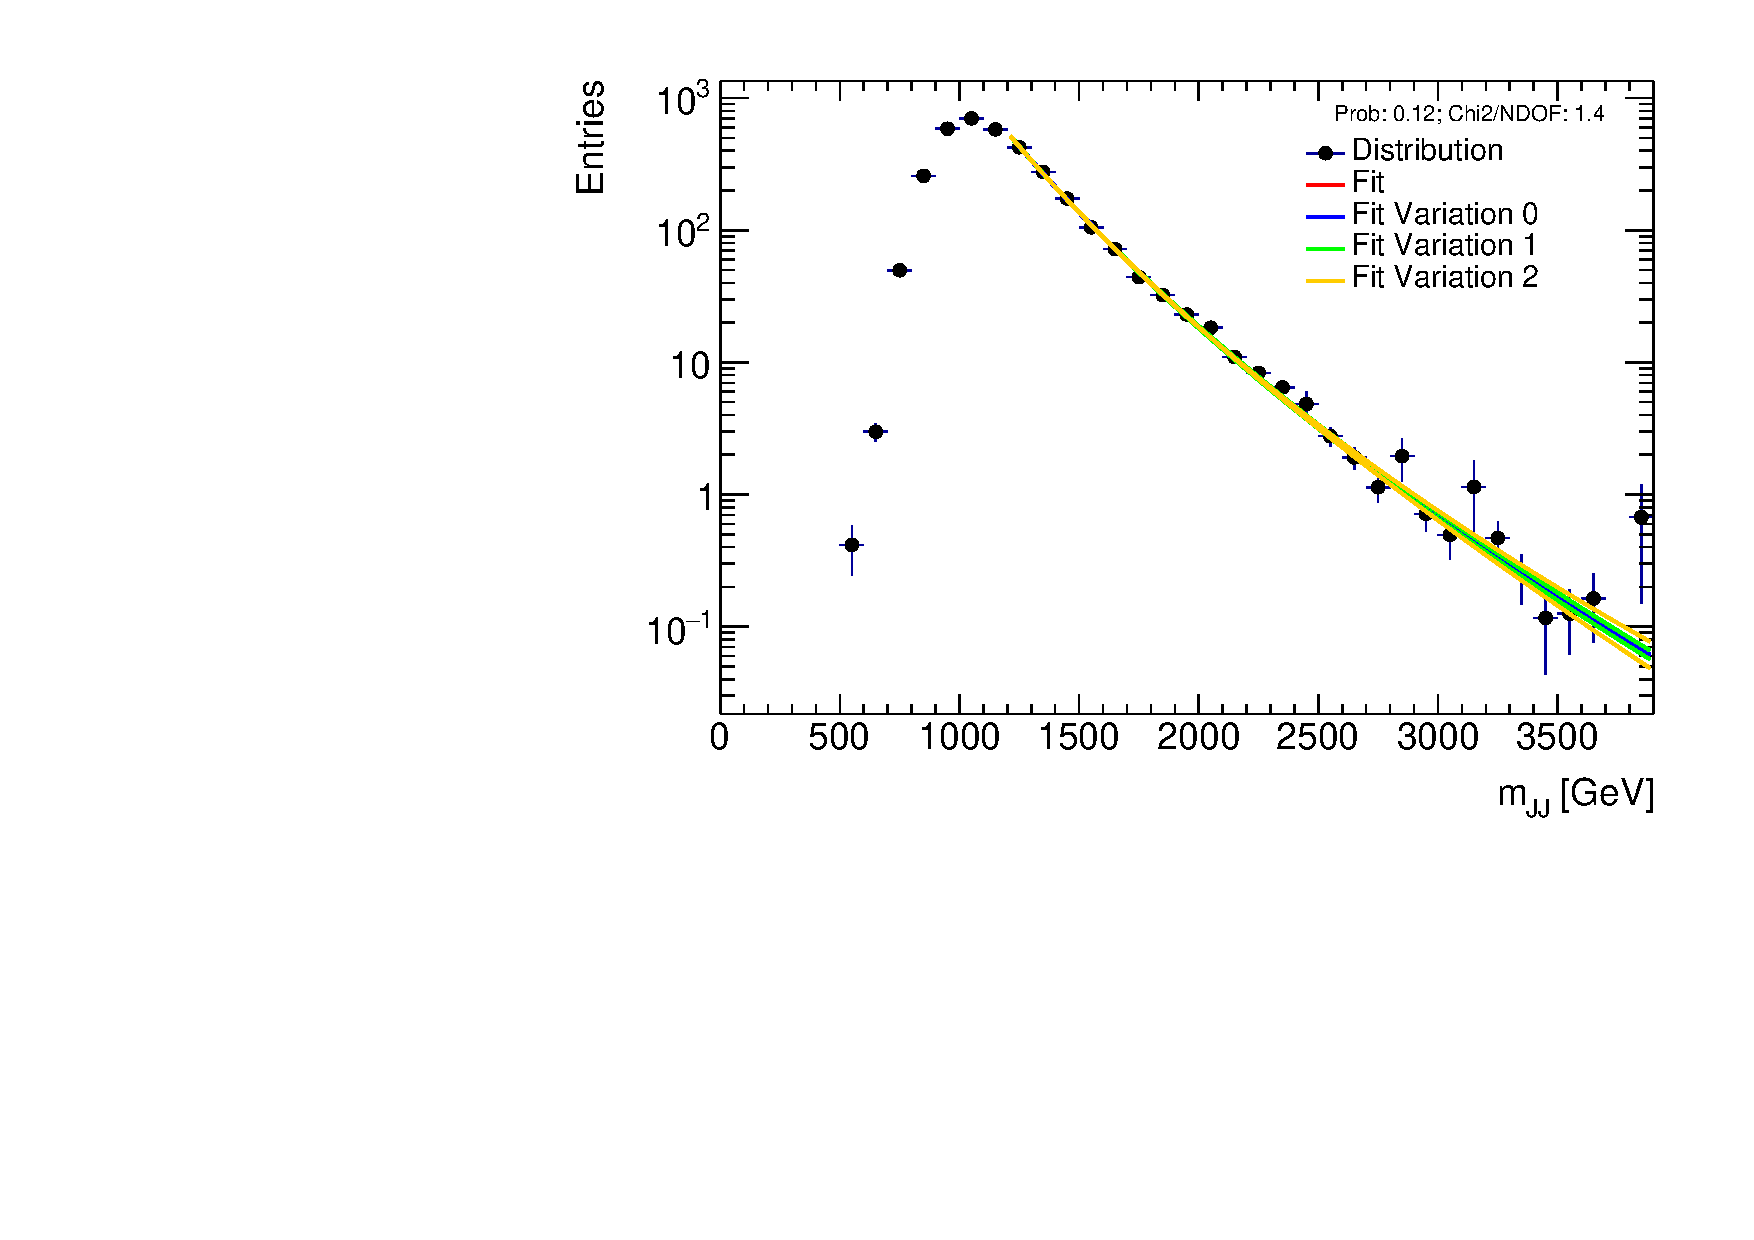
\includegraphics[width=0.3\textwidth,angle=-90]{figures/boosted/Smooth/qcd_est_TwoTag_split_Signal_mHH_pole_l.pdf}
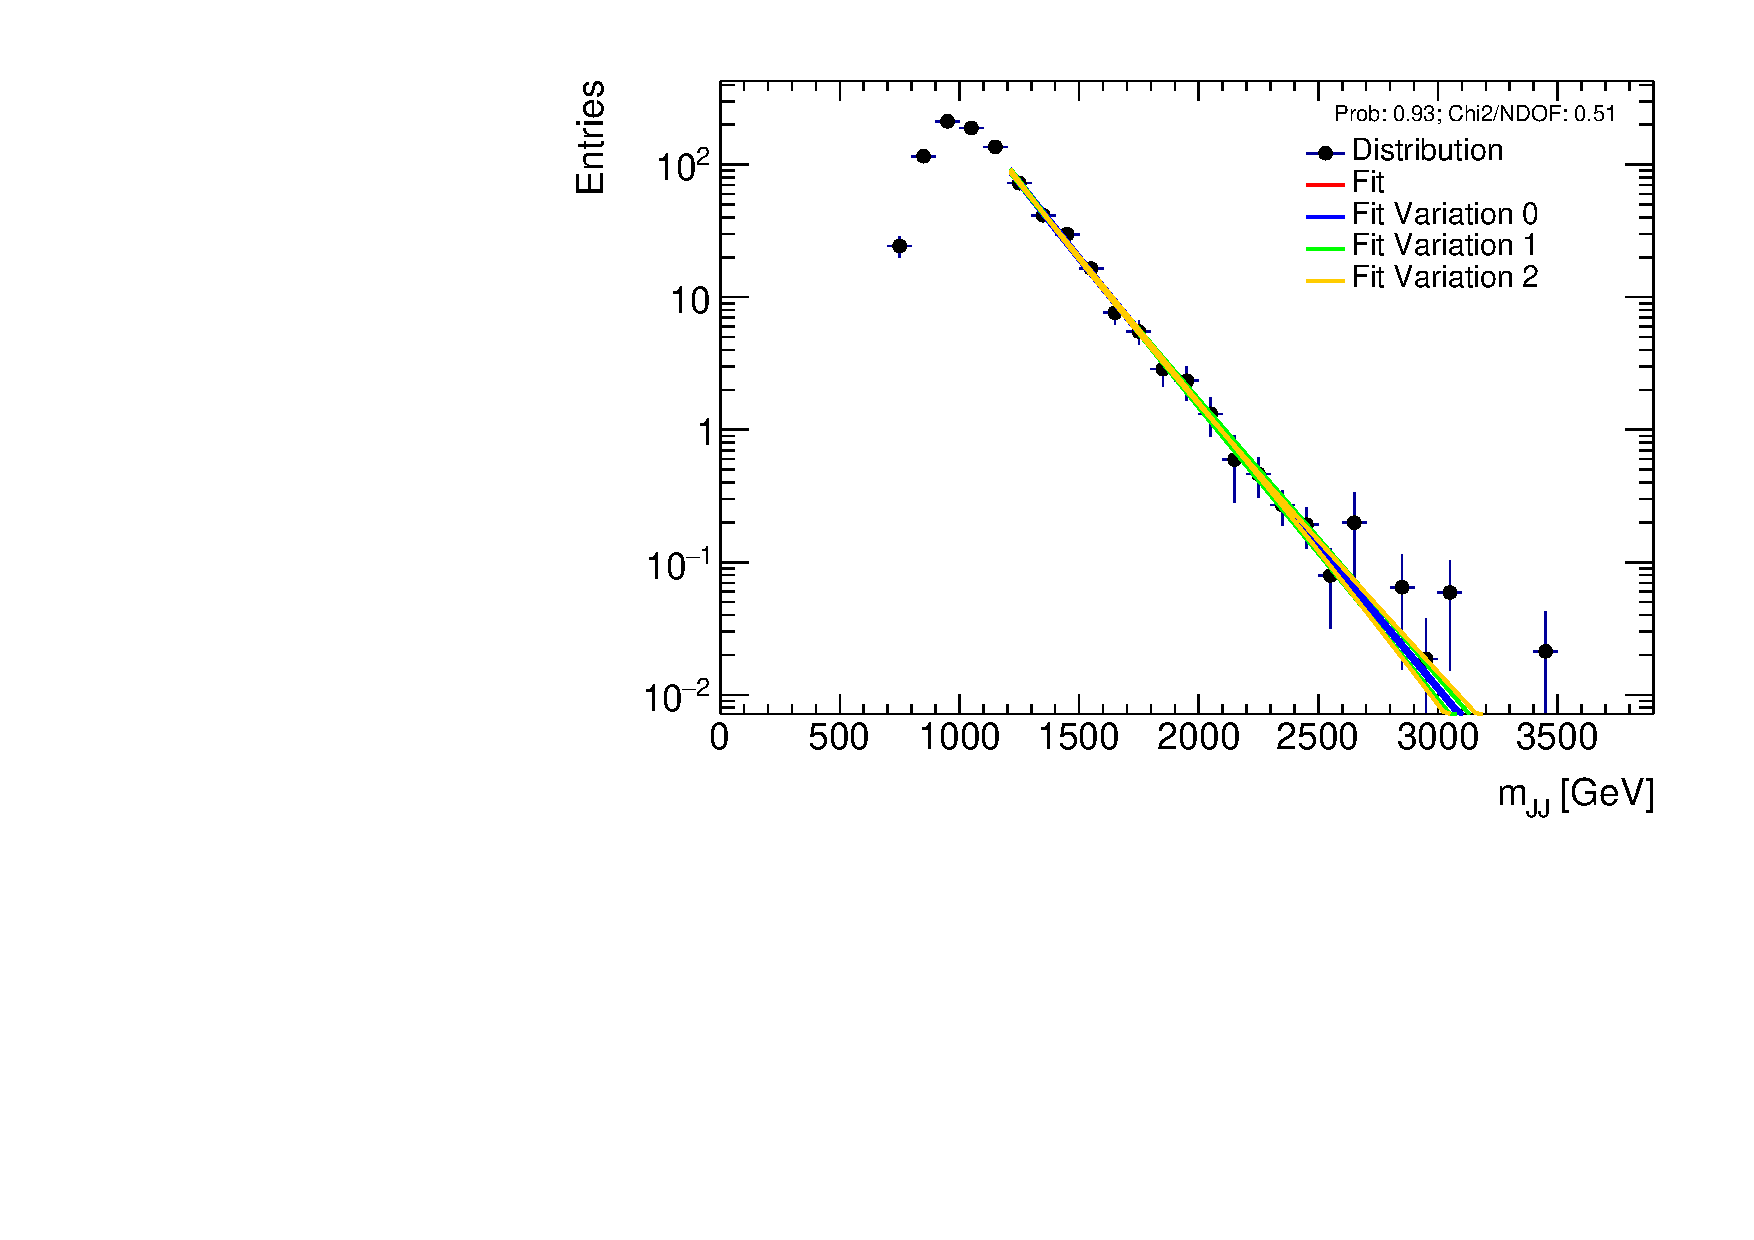
\includegraphics[width=0.3\textwidth,angle=-90]{figures/boosted/Smooth/ttbar_est_TwoTag_split_Signal_mHH_pole_l.pdf}\\
\caption{Fits for scaled background smoothing are shown for QCD (left column) and $t\bar{t}$ (right column) in the $4b$ (top), $3b$ (middle), and $2bs$ (bottom) signal region.  The left figures show the distributions with linear $y$-axis scale along with the fit central value and variations. The right figures show the  distributions with log $y$-axis scale along with the fit central value and the fit variations as determined by the varying the fit parameters within uncertainties whilst taking into account parameter correlations. }
\label{fig:signal-region-mjjscaled-smoothing}
\end{center}
\end{figure}


\begin{figure}[htbp!]
\begin{center}
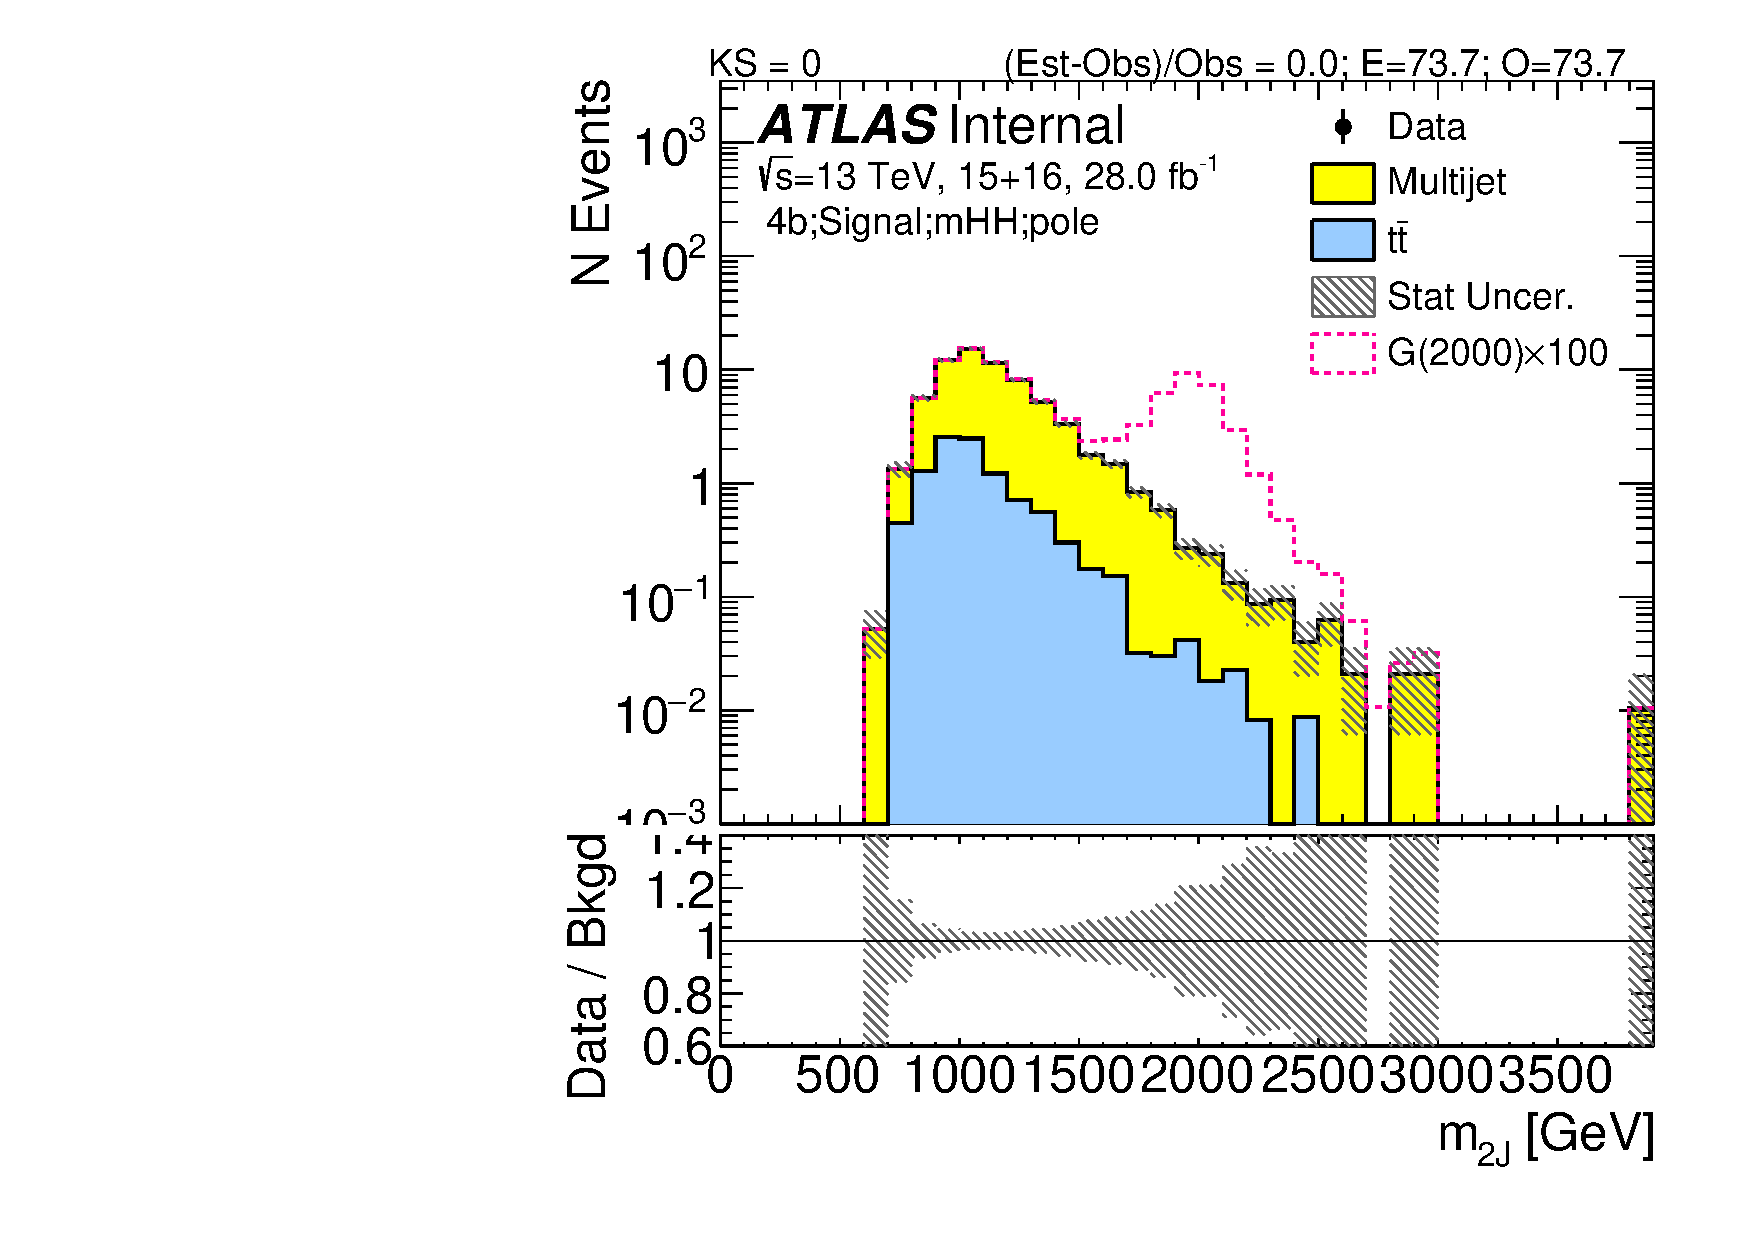
\includegraphics[width=0.3\textwidth,angle=-90]{figures/boosted/Signal/b77_FourTag_Signal_mHH_pole_1_blind.pdf}
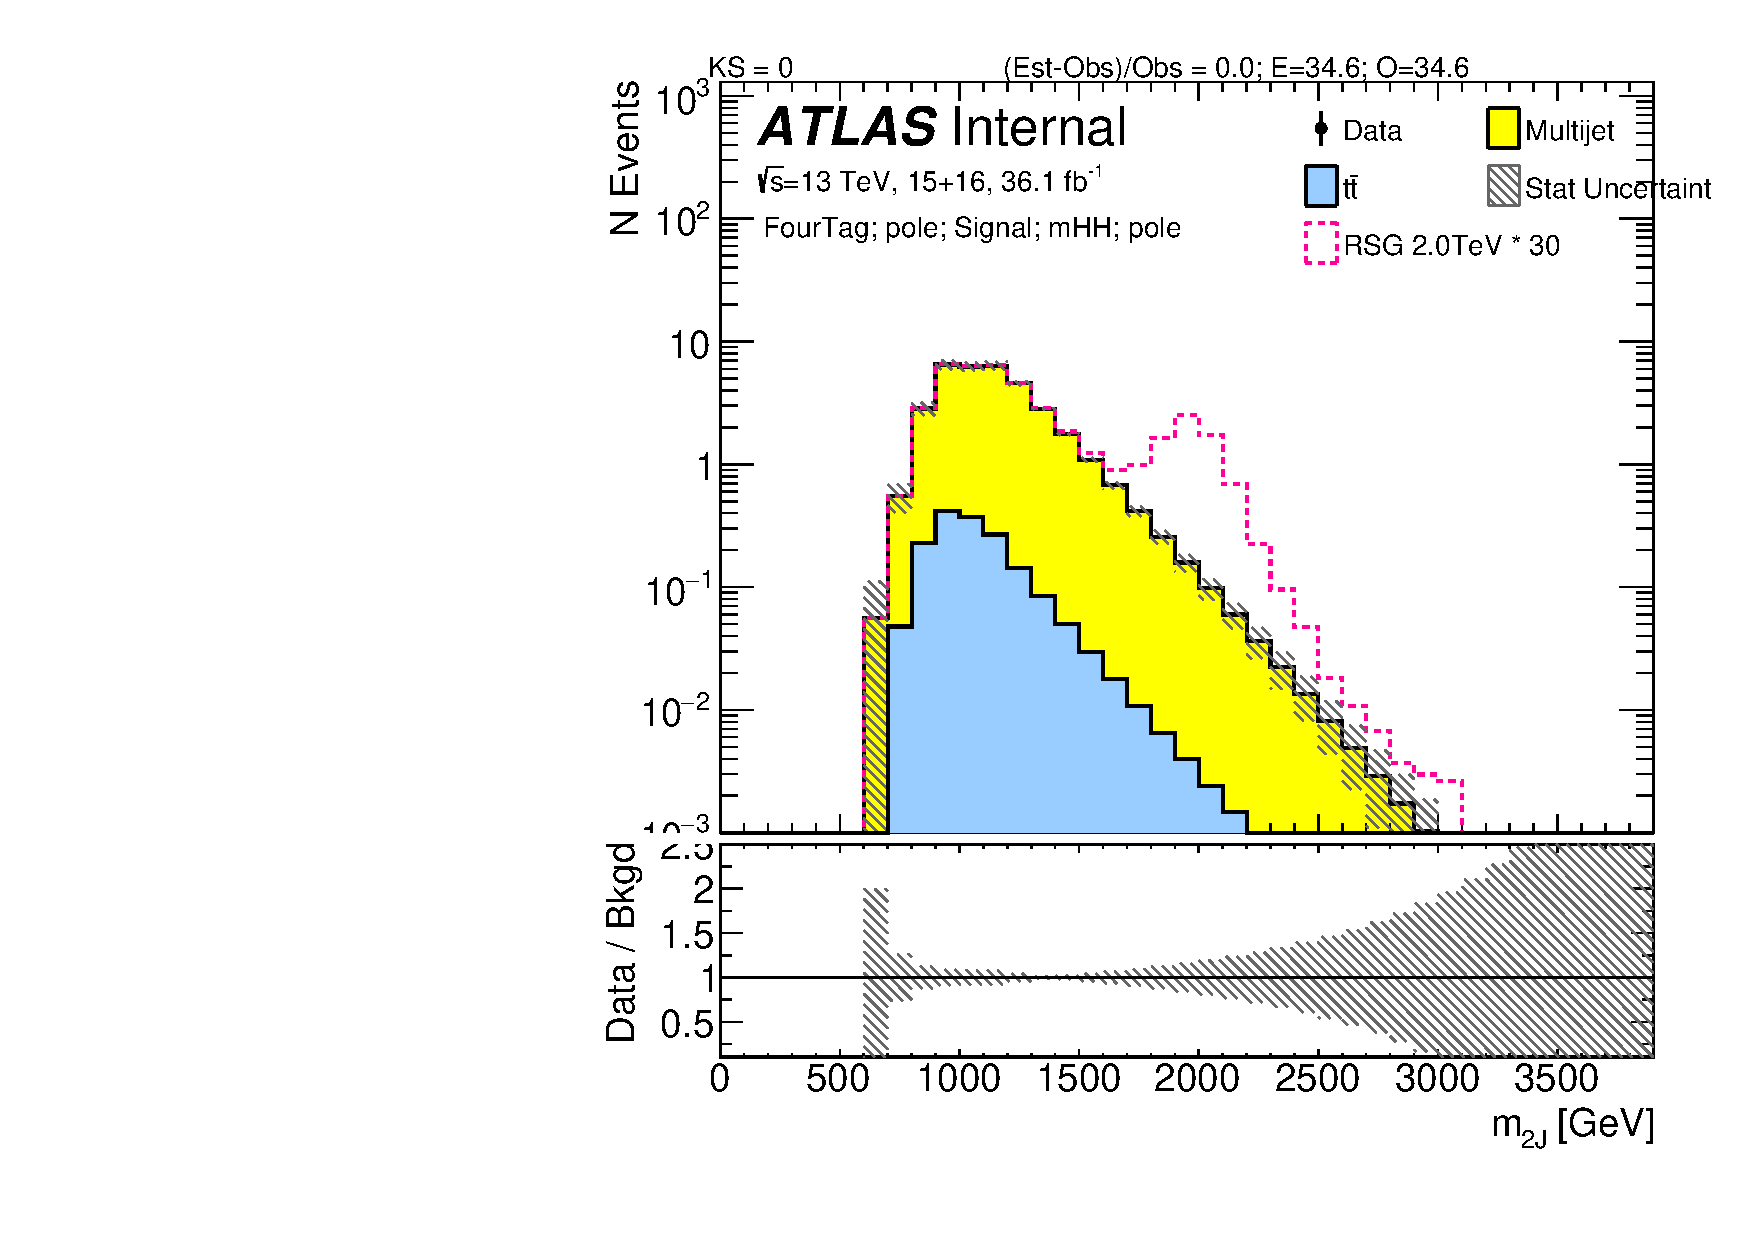
\includegraphics[width=0.3\textwidth,angle=-90]{figures/boosted/Smooth/Moriond_bkg_9_FourTag_pole_Signal_mHH_pole_1_blind.pdf}\\
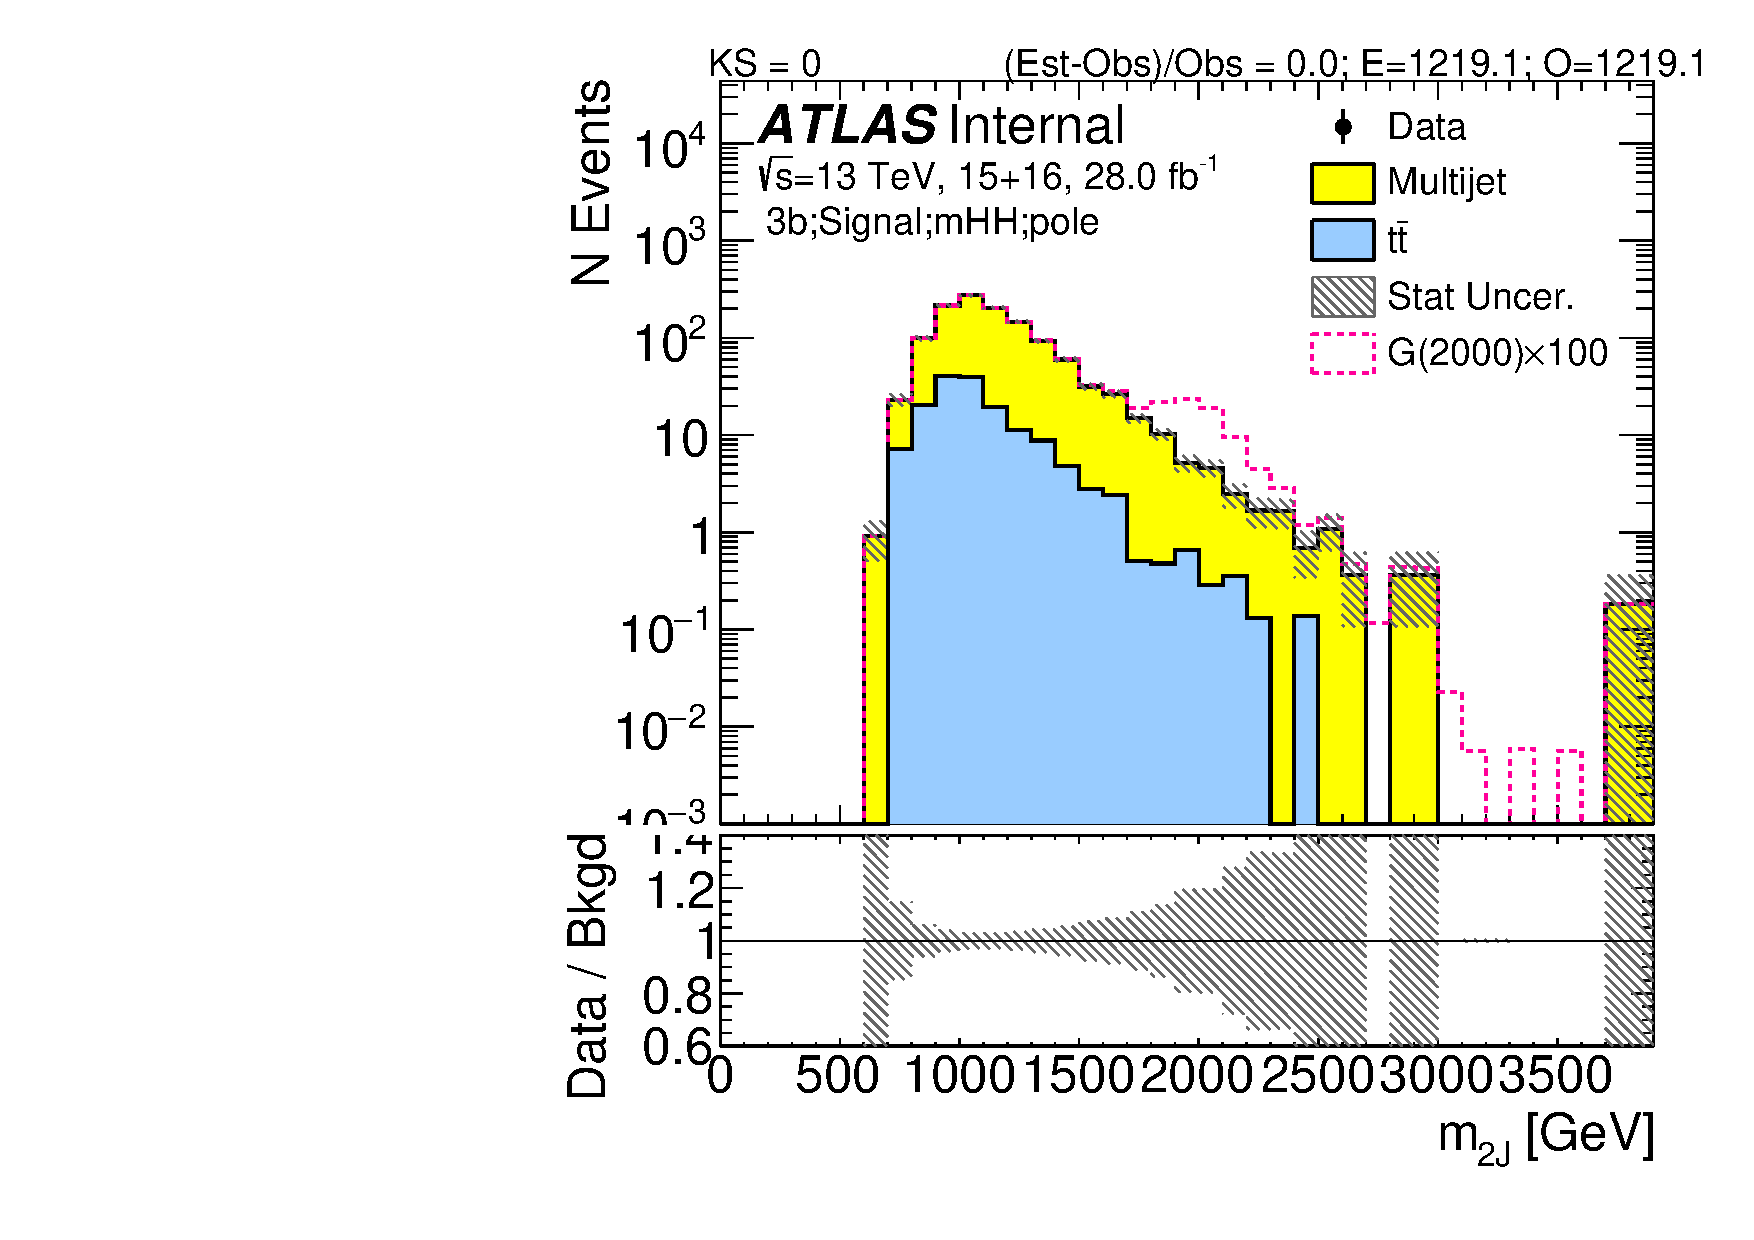
\includegraphics[width=0.3\textwidth,angle=-90]{figures/boosted/Signal/b77_ThreeTag_Signal_mHH_pole_1_blind.pdf}
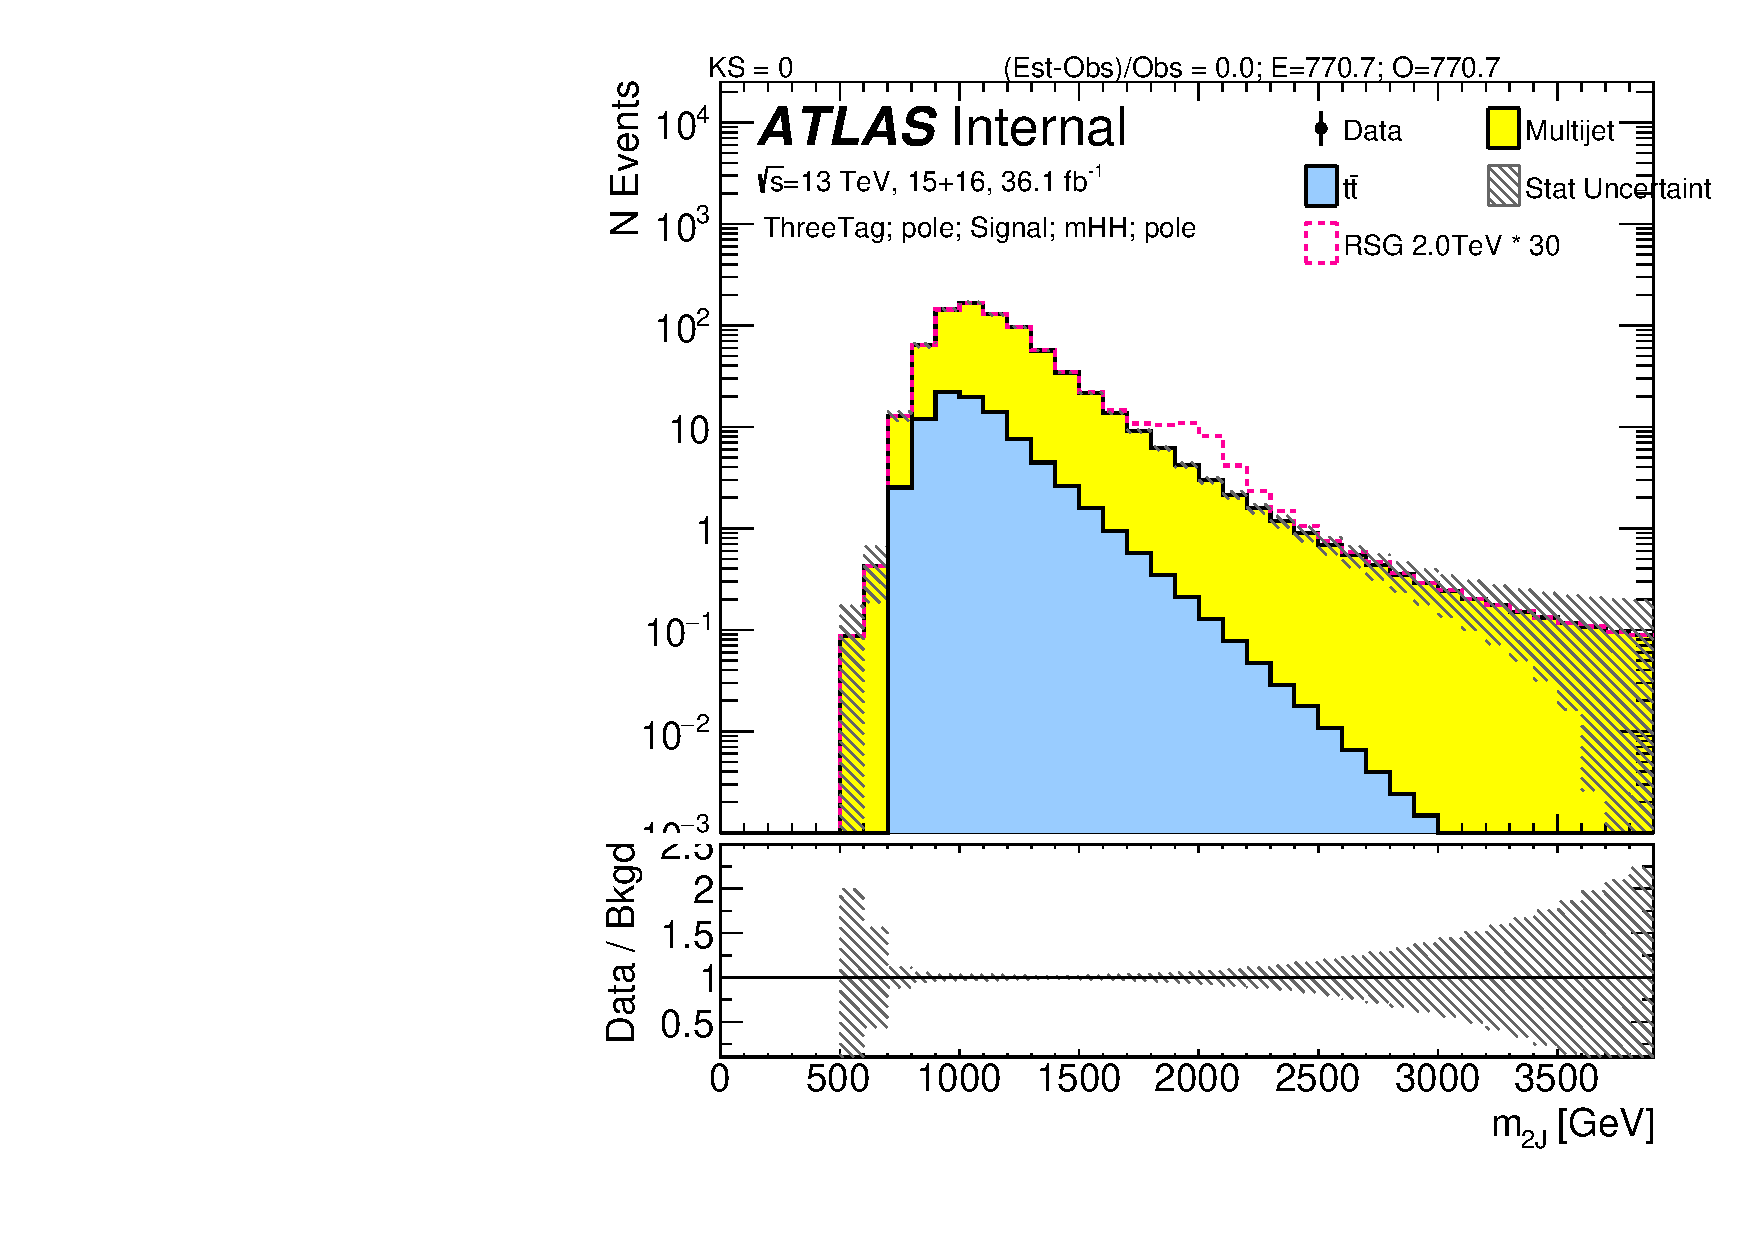
\includegraphics[width=0.3\textwidth,angle=-90]{figures/boosted/Smooth/Moriond_bkg_9_ThreeTag_pole_Signal_mHH_pole_1_blind.pdf}\\
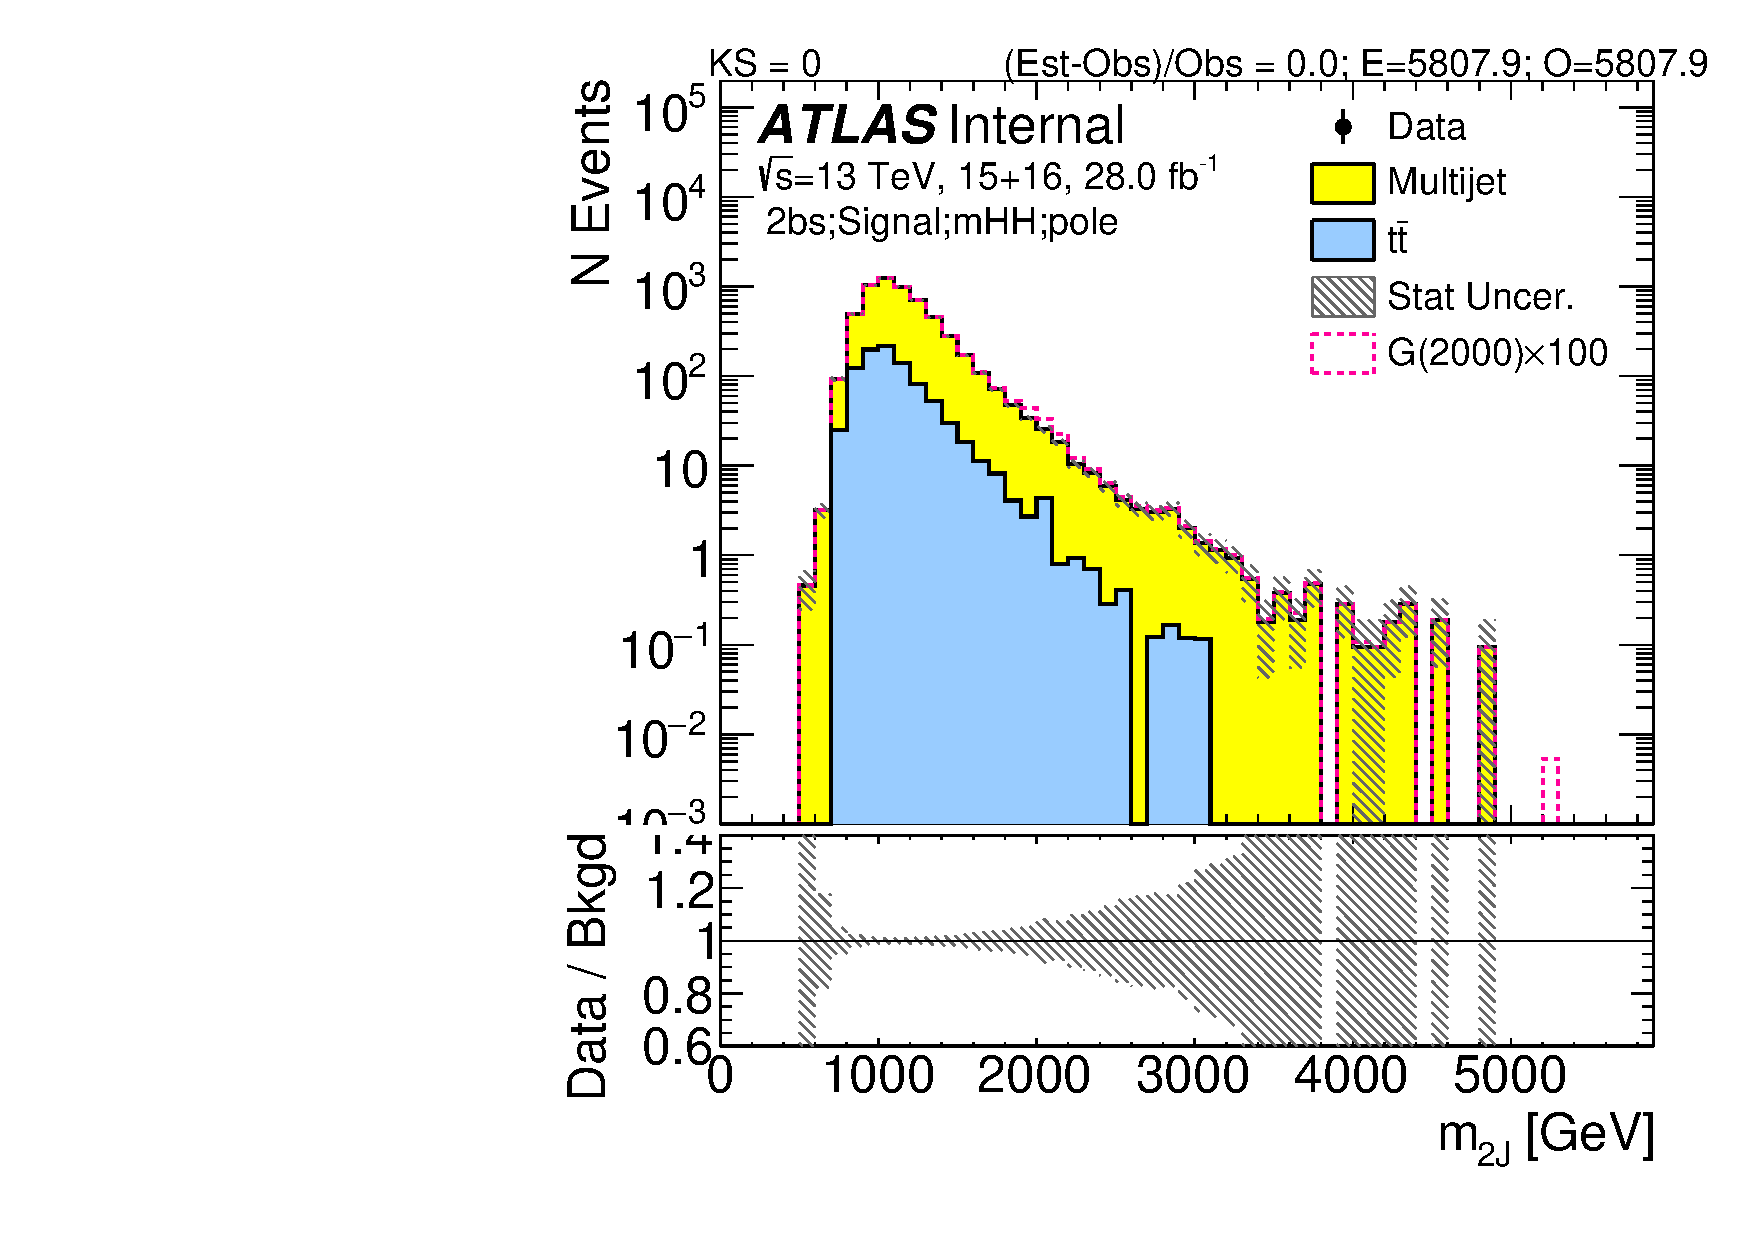
\includegraphics[width=0.3\textwidth,angle=-90]{figures/boosted/Signal/b77_TwoTag_split_Signal_mHH_pole_1_blind.pdf}
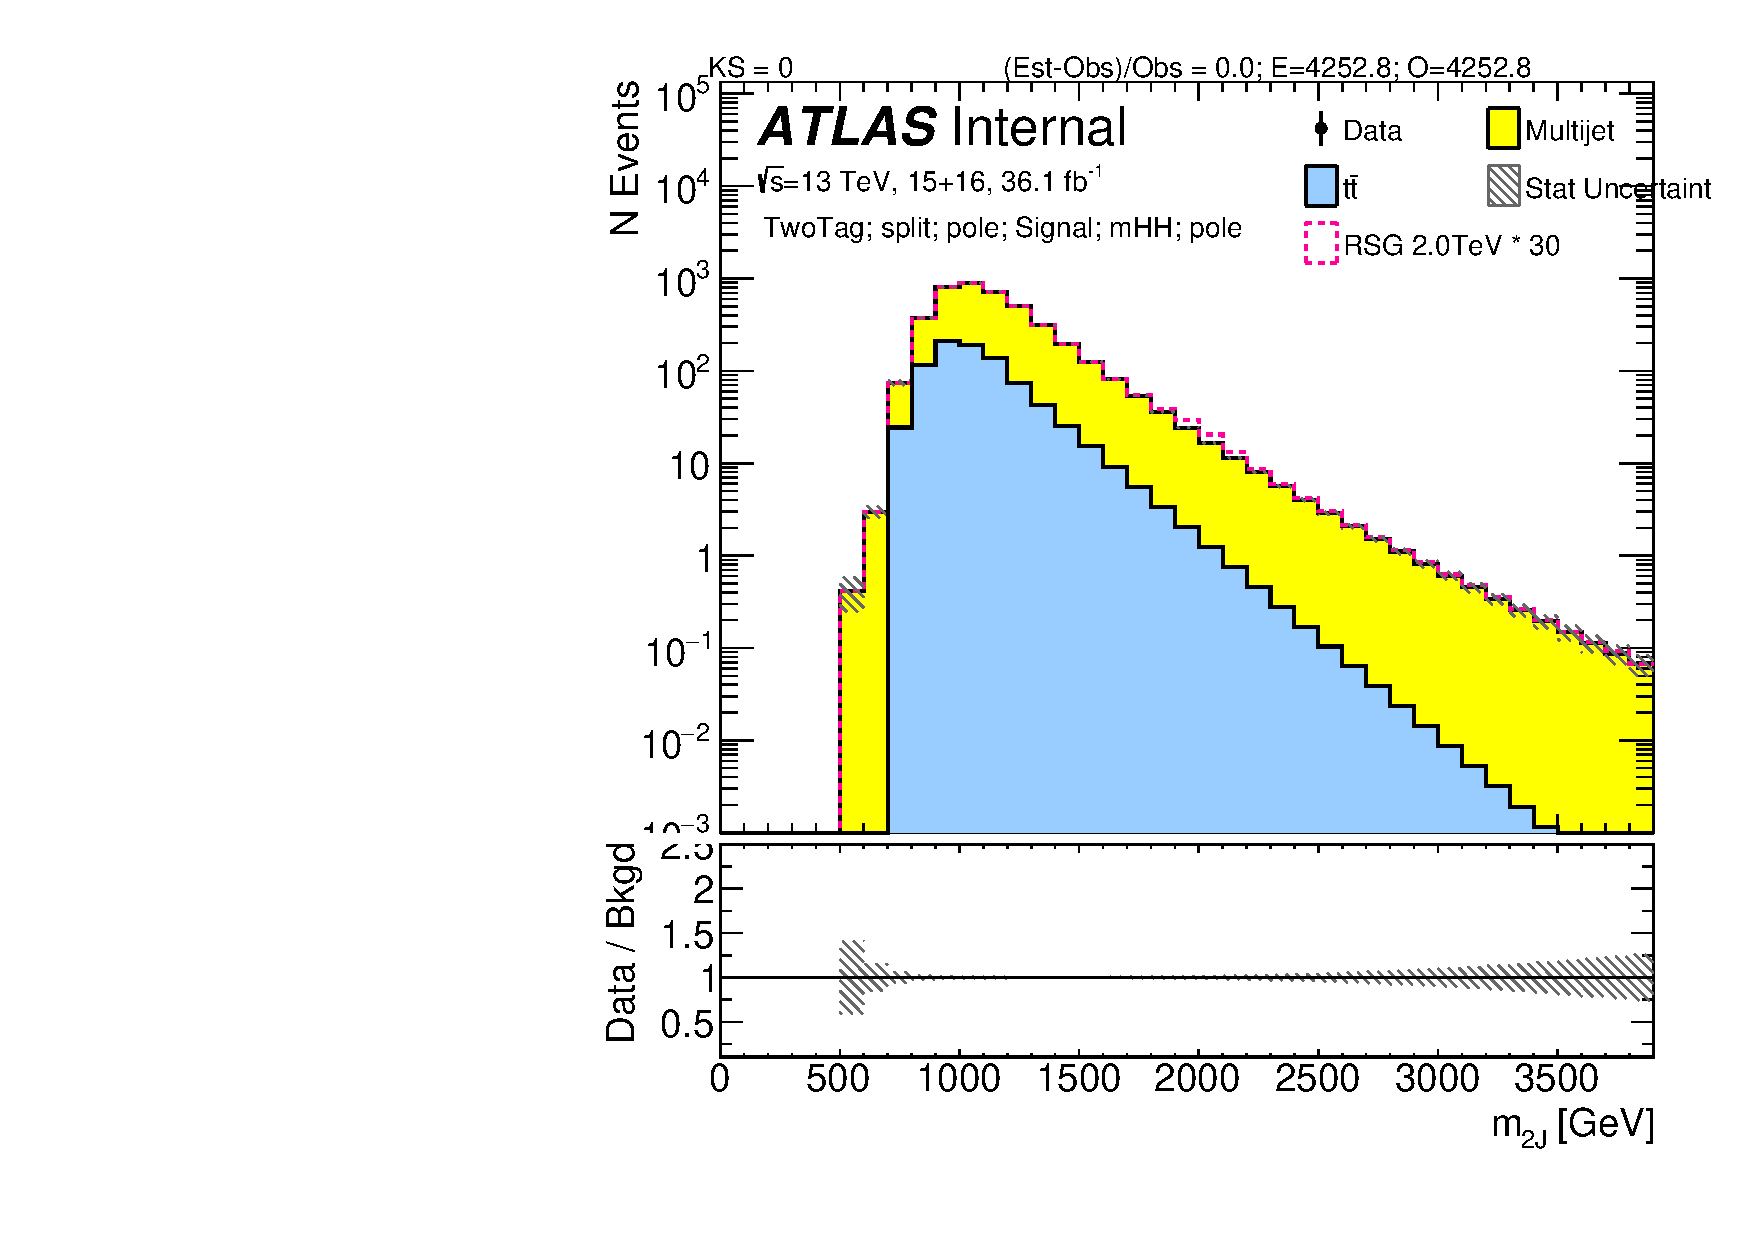
\includegraphics[width=0.3\textwidth,angle=-90]{figures/boosted/Smooth/Moriond_bkg_9_TwoTag_split_pole_Signal_mHH_pole_1_blind.pdf}
\end{center}
\caption{Background prediction for $4b$ (top), $3b$ (middle), and $2bs$ (bottom) signal region using scaled di-jet mass before (left) and after smoothing (right). The uncertainty band includes only fit statistical uncertainties.}
\label{fig:signal-region-mjjscaled-smooth-bkg-noSYS}
\end{figure}

%%%%%%%%%%%%%%%%%%%%%%%%%%%%%%%%%%%%%%%%%%%%%%%%%%%%%%%%%%%%%%%%%%%%%%%
%%%%%%%%%%%%%%%%%%%%%%%%%%%%%%%%%%%%%%%%%%%%%%%%%%%%%%%%%%%%%%%%%%%%%%%
%%%  Yields
%%%%%%%%%%%%%%%%%%%%%%%%%%%%%%%%%%%%%%%%%%%%%%%%%%%%%%%%%%%%%%%%%%%%%%%
%%%%%%%%%%%%%%%%%%%%%%%%%%%%%%%%%%%%%%%%%%%%%%%%%%%%%%%%%%%%%%%%%%%%%%%
\section{Yields}
\label{sec:yields}
\paragraph{}
The event yield results showing the estimated backgrounds, the signal predictions, and the observed data in the $4b$ and $3b$ and $2bs$ signal regions, control regions, and sideband regions can be found in Table~\ref{tab:yields4b} and Table~\ref{tab:yields3b} and Table~\ref{tab:yields2b} respectively. 
Total background statistical uncertainty is less than the quadratic sum of \ttbar~ and QCD because of the anti-correlation.
Z+jets have a negligible yield in the signal regions, therefore, in the later chapters, it is not included in the figures and tables.

\begin{table}[htbp!]
\footnotesize
\begin{center}
\caption{Expected yields for backgrounds in the $4b$ signal region, control region, and sideband region, along with the observed number of data events.  The signal predictions for \Grav $m=1.0, 1.5, 2.0$~\TeV\ with $c=1.0$. The uncertainty listed is statistical, without fit uncertainty.}
\begin{footnotesize} 
\begin{tabular}{c|c|c|c} 
FourTag & Sideband & Control & Signal \\ 
\hline\hline 
& & & \\ 
QCD Est & 176.26 $\pm$ 2.96 & 64.21 $\pm$ 1.79 & 32.91 $\pm$ 1.25\\ 
$t\bar{t}$ Est.  & 27.86 $\pm$ 0.25 & 6.38 $\pm$ 0.13 & 1.68 $\pm$ 0.044\\ 
$Z+jets$ & 0 $\pm$ 0 & 6.18 $\pm$ 5.12 & 0 $\pm$ 0\\ 
Total Bkg Est & 204.12 $\pm$ 2.97 & 76.77 $\pm$ 5.43 & 34.59 $\pm$ 1.25\\ 
Data & 204.0 $\pm$ 14.28 & 81.0 $\pm$ 9.0 & 0 $\pm$ 0\\ 
$c=1.0$,$m=1.0TeV$ & 2.52 $\pm$ 0.1 & 5.4 $\pm$ 0.15 & 10.07 $\pm$ 0.2\\ 
$c=1.0$,$m=2.0TeV$ & 0.034 $\pm$ 0.0015 & 0.1 $\pm$ 0.0026 & 0.25 $\pm$ 0.0041\\ 
$c=1.0$,$m=3.0TeV$ & 0.00032 $\pm$ 3.7e-05 & 0.0008 $\pm$ 5.6e-05 & 0.0016 $\pm$ 8e-05\\ 
& & & \\ 
\hline\hline 
\end{tabular} 
\end{footnotesize} 
\newline 

\label{tab:yields4b}
\end{center}
\end{table}


\begin{table}[htbp!]
\footnotesize
\begin{center}
\caption{Expected yields for backgrounds in the $3b$ signal region, control region, and sideband region, along with the observed number of data events.  The signal predictions for \Grav $m=1.0, 1.5, 2.0$~\TeV\ with $c=1.0$. The uncertainty listed is statistical, without fit uncertainty.}
\begin{footnotesize} 
\begin{tabular}{c|c|c|c} 
ThreeTag & Sideband & Control & Signal \\ 
\hline\hline 
& & & \\ 
QCD Est & 3518.01 $\pm$ 27.48 & 1413.52 $\pm$ 17.36 & 701.6 $\pm$ 11.95\\ 
$t\bar{t}$ Est.  & 852.88 $\pm$ 25.72 & 162.31 $\pm$ 11.15 & 79.34 $\pm$ 2.05\\ 
$Z+jets$ & 32.8 $\pm$ 11.34 & 11.21 $\pm$ 5.65 & 0.49 $\pm$ 0.49\\ 
Total Bkg Est & 4403.69 $\pm$ 39.31 & 1587.04 $\pm$ 21.4 & 781.42 $\pm$ 12.14\\ 
Data & 4403.0 $\pm$ 66.36 & 1553.0 $\pm$ 39.41 & 801.0 $\pm$ 28.3\\ 
$c=1.0$,$m=1.0TeV$ & 7.86 $\pm$ 0.18 & 12.58 $\pm$ 0.23 & 26.0 $\pm$ 0.33\\ 
$c=1.0$,$m=2.0TeV$ & 0.16 $\pm$ 0.0035 & 0.38 $\pm$ 0.0054 & 0.76 $\pm$ 0.0076\\ 
$c=1.0$,$m=3.0TeV$ & 0.0036 $\pm$ 0.00013 & 0.0075 $\pm$ 0.00018 & 0.013 $\pm$ 0.00023\\ 
& & & \\ 
\hline\hline 
\end{tabular} 
\end{footnotesize} 
\newline 

\label{tab:yields3b}
\end{center}
\end{table}

\begin{table}[htbp!]
\footnotesize
\begin{center}
\caption{Expected yields for backgrounds in the $2bs$ signal region, control region, and sideband region, along with the observed number of data events.  The signal predictions for \Grav $m=1.0, 1.5, 2.0$~\TeV\ with $c=1.0$. The uncertainty listed is statistical, without fit uncertainty.}
\begin{footnotesize} 
\begin{tabular}{c|c|c|c} 
TwoTag split & Sideband & Control & Signal \\ 
\hline\hline 
& & & \\ 
QCD Est & 17216.91 $\pm$ 38.33 & 6821.96 $\pm$ 23.49 & 3393.56 $\pm$ 16.64\\ 
$t\bar{t}$ Est.  & 7852.35 $\pm$ 70.3 & 1484.57 $\pm$ 29.24 & 858.27 $\pm$ 22.23\\ 
$Z+jets$ & 67.74 $\pm$ 16.82 & 26.44 $\pm$ 10.08 & 0.13 $\pm$ 0.091\\ 
Total Bkg Est & 25137.01 $\pm$ 81.82 & 8332.97 $\pm$ 38.84 & 4251.96 $\pm$ 27.77\\ 
Data & 25137.0 $\pm$ 158.55 & 8486.0 $\pm$ 92.12 & 4376.0 $\pm$ 66.15\\ 
$c=1.0$,$m=1.0TeV$ & 4.79 $\pm$ 0.14 & 6.33 $\pm$ 0.16 & 10.87 $\pm$ 0.22\\ 
$c=1.0$,$m=2.0TeV$ & 0.18 $\pm$ 0.0039 & 0.36 $\pm$ 0.0056 & 0.6 $\pm$ 0.0072\\ 
$c=1.0$,$m=3.0TeV$ & 0.013 $\pm$ 0.00025 & 0.027 $\pm$ 0.00034 & 0.039 $\pm$ 0.00041\\ 
& & & \\ 
\hline\hline 
\end{tabular} 
\end{footnotesize} 
\newline 

\label{tab:yields2b}
\end{center}
\end{table}
